\documentclass[handout]{beamer}
%\documentclass{beamer}
\usetheme{Marburg}
\useoutertheme{infolines}
\newcommand{\answers}{1}

\usepackage{amsmath}
\usepackage{caption}
\usepackage{color}
\usepackage{enumerate}
\usepackage{listings}
\usepackage{hyperref}
\usepackage{mathrsfs}
\usepackage{natbib}
\usepackage{url}

\providecommand{\all}{\ \forall \ }
\providecommand{\bs}{\backslash}
\providecommand{\e}{\varepsilon}
\providecommand{\E}{\ \exists \ }
\providecommand{\lm}[2]{\lim_{#1 \rightarrow #2}}
\providecommand{\m}[1]{\mathbb{#1}}
\providecommand{\nv}{{}^{-1}}
\providecommand{\ov}[1]{\overline{#1}}
\providecommand{\p}{\newpage}
\providecommand{\q}{$\quad$ \newline}
\providecommand{\rt}{\rightarrow}
\providecommand{\Rt}{\Rightarrow}
\providecommand{\vc}[1]{\boldsymbol{#1}}
\providecommand{\wh}[1]{\widehat{#1}}

\hypersetup{colorlinks,linkcolor=,urlcolor=blue}
\numberwithin{equation}{section}

\definecolor{dkgreen}{rgb}{0,0.6,0}
\definecolor{gray}{rgb}{0.5,0.5,0.5}
\definecolor{mauve}{rgb}{0.58,0,0.82}

\lstset{ 
  language=C,                % the language of the code
  basicstyle= \tiny,           % the size of the fonts that are used for the code
  numbers=left,
  numberfirstline=true,
  numbersep=5pt,                  % how far the line-numbers are from the code
  backgroundcolor=\color{white},      % choose the background color. You must add \usepackage{color}
  showspaces=false,               % show spaces adding particular underscores
  showstringspaces=false,         % underline spaces within strings
  showtabs=false,                 % show tabs within strings adding particular underscores
  frame=lrb,                   % adds a frame around the code
  rulecolor=\color{black},        % if not set, the frame-color may be changed on line-breaks within not-black text 
  tabsize=2,                      % sets default tabsize to 2 spaces
  captionpos=t,                   % sets the caption-position 
  breaklines=true,                % sets automatic line breaking
  breakatwhitespace=false,        % sets if automatic breaks should only happen at whitespace
  %title=\lstname,                   % show the filename of files included with \lstinputlisting;
  keywordstyle=\color{blue},          % keyword style
  commentstyle=\color{gray},       % comment style
  stringstyle=\color{dkgreen},         % string literal style
  escapeinside={\%*}{*)},            % if you want to add LaTeX within your code
  morekeywords={*, ...},               % if you want to add more keywords to the set
  xleftmargin=0.053in, % left horizontal offset of caption box
  xrightmargin=-.03in % right horizontal offset of caption box
}

%\DeclareCaptionFont{white}{\color{white}}
%\DeclareCaptionFormat{listing}{\parbox{\textwidth}{\colorbox{gray}{\parbox{\textwidth}{#1#2#3}}\vskip-0.05in}}
%\captionsetup[lstlisting]{format = listing, labelfont = white, textfont = white}
%For caption-free listings, comment out the 3 lines above and uncomment the 2 lines below.
 \captionsetup{labelformat = empty, labelsep = none}
 \lstset{frame = single}

\title{A short course in GPU computing for statisticians}
\author{Will Landau}
\date{September 9, 2013}
\institute{Iowa State University}

\begin{document}

\begin{frame}
\titlepage
 \end{frame}
 
 \begin{frame}
\frametitle{Outline}
\tableofcontents
\end{frame}
 
 \AtBeginSection[]
{
   \begin{frame}
       \frametitle{Outline}
       \tableofcontents[currentsection]
   \end{frame}
}

\section{GPUs, parallelism, and why we care}

\begin{frame}[fragile]
\frametitle{The single instruction, multiple data (SIMD) paradigm}

\begin{itemize}
\pause \item SIMD: apply the same command to multiple places in a dataset. 

\lstset{basicstyle=\footnotesize}

\pause \begin{lstlisting}
for(i = 0; i < 1e6; ++i)
  a[i] = b[i] + c[i];
\end{lstlisting}


\pause \item On CPUs, the iterations of the loop run sequentially.

\pause \item With GPUs, we can easily run all 1,000,000 iterations simultaneously.

\pause \begin{lstlisting}
i = threadIdx.x;
a[i] = b[i] + c[i];
\end{lstlisting}

\pause \item We can similarly \emph{parallelize} a lot more than just loops.
\end{itemize}

\lstset{basicstyle=\tiny}
\end{frame}





\begin{frame}
\frametitle{Parallel MCMC by Lee, Yau, Giles, and others}

\scriptsize
\begin{center}
\begin{tabular}{llll}
\# chains & CPU time (min) & GTX 280 (min) & CPU time / GPU time \\ \hline
8 & 0.0166 & 0.0148 & 1.1 \\
32 & 0.0656 & 0.0151 & 4 \\
128 & 0.262 & .0154 & 17 \\
512 & 1.04 & 0.0174  & 60 \\
2,048 & 4.16 & 0.0248 & 168 \\
8,192 & 16.64 & 0.0720 & 230 \\
32,768 & 66.7 & 0.249 & 268 \\
131,072 & 270.3 & 0.970 & 279
\end{tabular}
\end{center}

\end{frame}



\begin{frame}
\frametitle{Parallel sequential MC by Lee, Yau, Giles, and others}


\scriptsize
\begin{center}
\begin{tabular}{llll}
Sample size & CPU time (min) & GTX 280 (min) & CPU time / GPU time \\ \hline
8,192 & 4.44 & 0.0199 & 223.1 \\
16,384 & 8.82 & 0.0355 & 263 \\
32,768 & 17.7 & 0.0666 & 265 \\
65,536 & 35.3 & 0.131 & 269 \\
131,076 & 70.6 & 0.261 & 270.5 \\
262,144 & 141 & 0.52 & 271.2
\end{tabular}
\end{center}
\end{frame}


\begin{frame}
\frametitle{Parallel Bayesian EM by Suchard, Wang, Chan, and others}

\scriptsize
\begin{center}
\begin{tabular}{llll}
Sample size & cpu 1 (sec) & gpu 1 (sec) & CPU time / GPU Time \\ \hline
$10^2$ & 4.0 & 71.1 & 0.1 \\
$10^3$ & 40.0 &  81.3  & 0.5 \\
$10^4$ & 607.0 & 91.2  & 6.7 \\
$10^5$ & 7793.0 & 129.6  & 60.1 \\
$10^6$ & 78765.0 & 680.6  & 115.7 \\
\end{tabular}
\end{center}

\end{frame}

\begin{frame}
\frametitle{Other applications}
\begin{itemize}
\item Clustering
\pause \item Bootstrap
\pause \item Regression
\pause \item Matrix algebra
\pause \item EM Algorithm
\pause \item Rejection sampling 
\pause \item Multiple testing
\pause \item Cross validation
\item $\cdots$
\end{itemize}

\end{frame}

\begin{frame}
\frametitle{Computer processors}
\begin{itemize}
\item {\bf Processing unit}: a computer chip that performs executive functions. 
\pause \item {\bf Core}: One of possibly many ``sub-processors" placed on the same processing unit, each of which has the full functionality of the processing unit.
\end{itemize}

\end{frame}


\begin{frame}
\frametitle{The Central Processing Unit (CPU)}

\begin{itemize}
\item Regular computer processor.
\pause \item Allows parallelism, but not \emph{massive} parallelism on its own.
\pause \item Usually contains 1 to 8 cores.
\pause \item Examples:
\begin{itemize}
\item Intel 8086 (1979, x86)
\pause \item Intel Core 2 Duo
\pause \item  Intel 80486DX2 (below)
\end{itemize}
\end{itemize}

\begin{center}
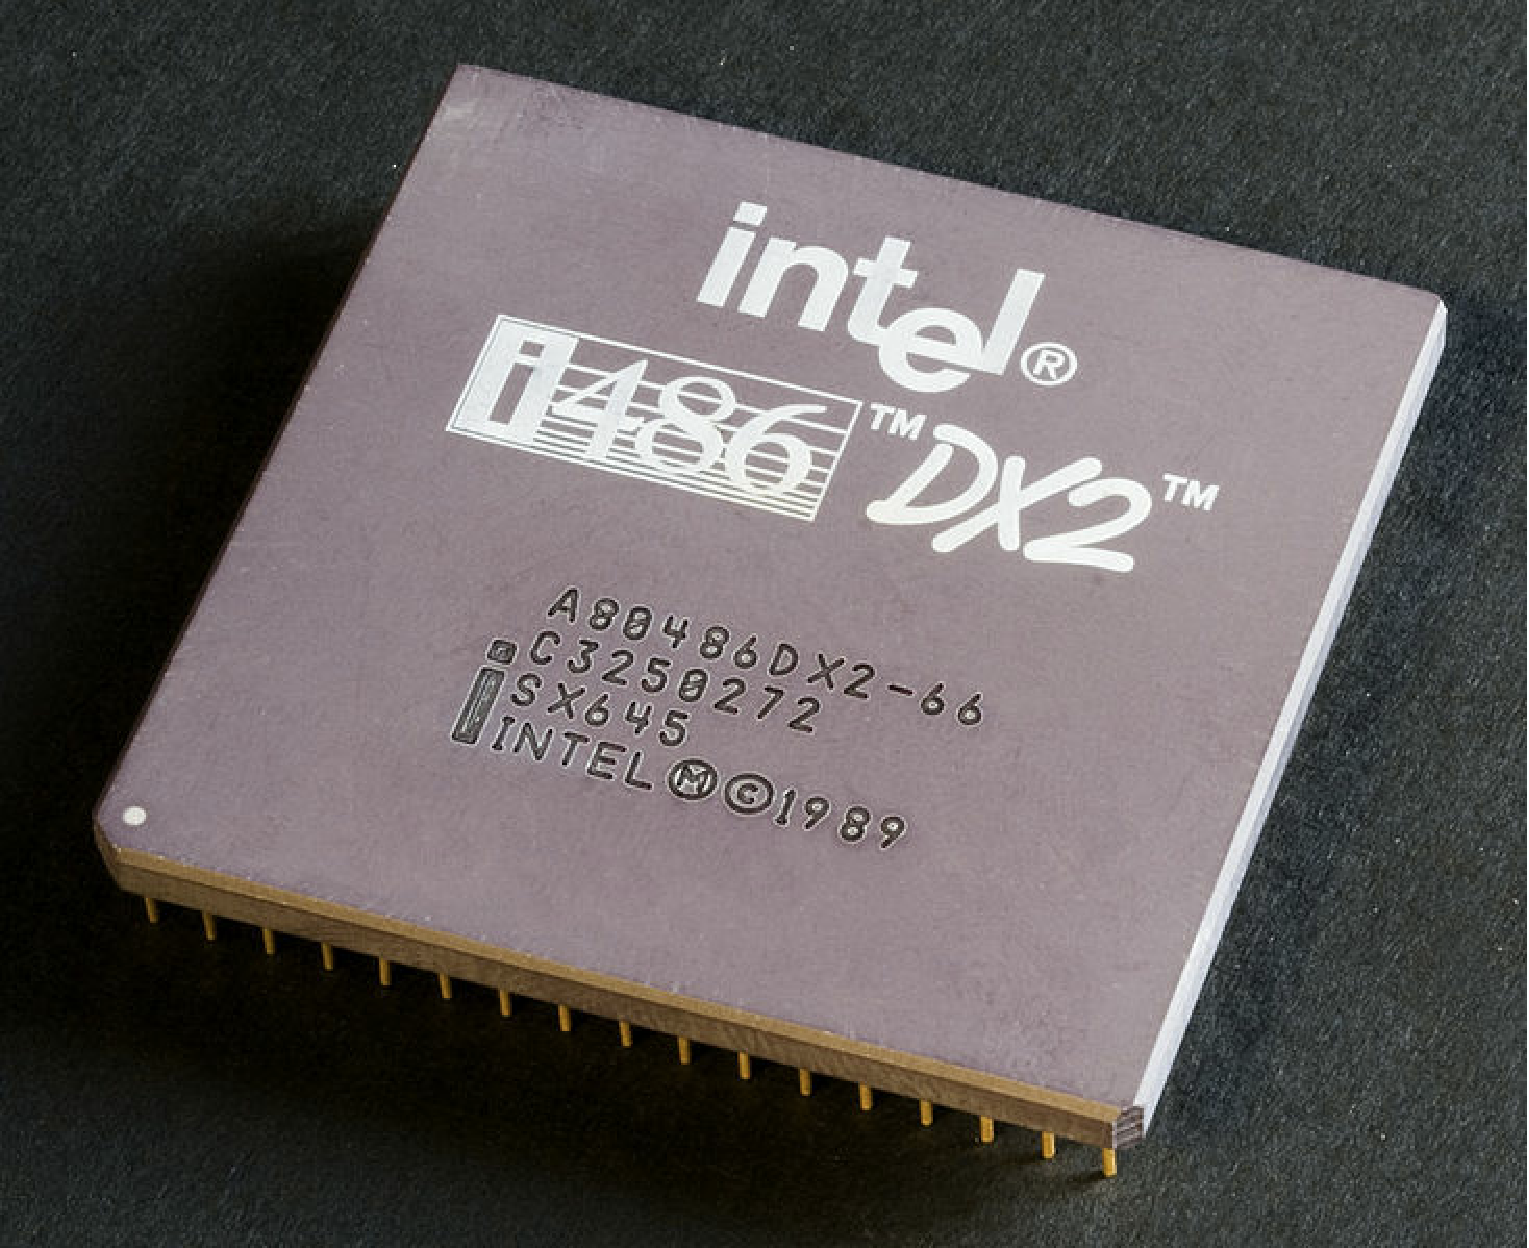
\includegraphics[scale = .175, angle = -1]{../../fig/cpu1} $\quad$ 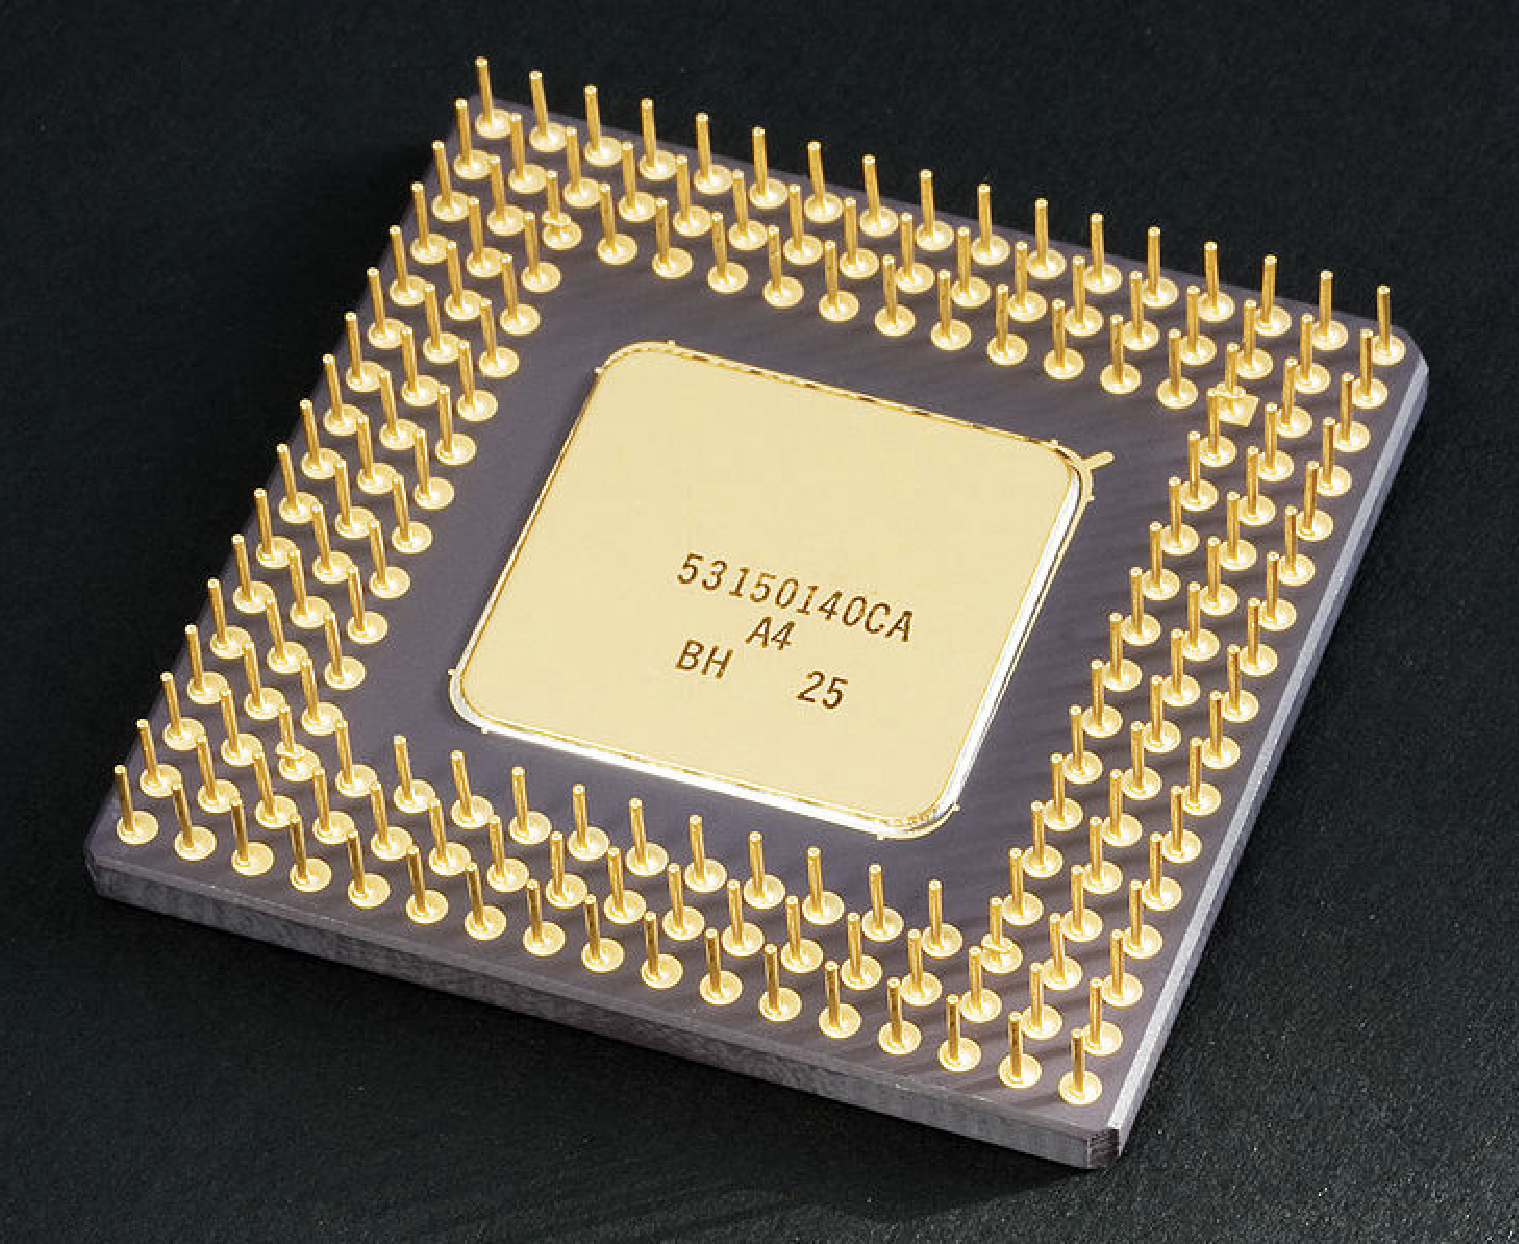
\includegraphics[scale = .175, angle = -1]{../../fig/cpu2}
\end{center}
\end{frame}



\begin{frame}
\frametitle{The Graphics Processing Unit (GPU)}
\scriptsize

\begin{itemize}\scriptsize
\item Processor in a video card or graphics card.
\pause \item Massively parallel: originally designed to speed up graphics throughput in video games.
\pause \item Cannot run by itself. Needs to be hooked up to a computer with a CPU.
\pause \item Contains several hundred cores.
\pause \item Higher memory bandwidth than a CPU.
\pause \item Examples:
\begin{itemize}\scriptsize
\item NVIDIA GeForce 6600 (bottom left)
\pause \item NVIDIA GeForce GTX 580 
\pause \item NVIDIA Tesla M2070 (on our GPU-enabled machines)
\end{itemize}

\end{itemize}

\begin{center}
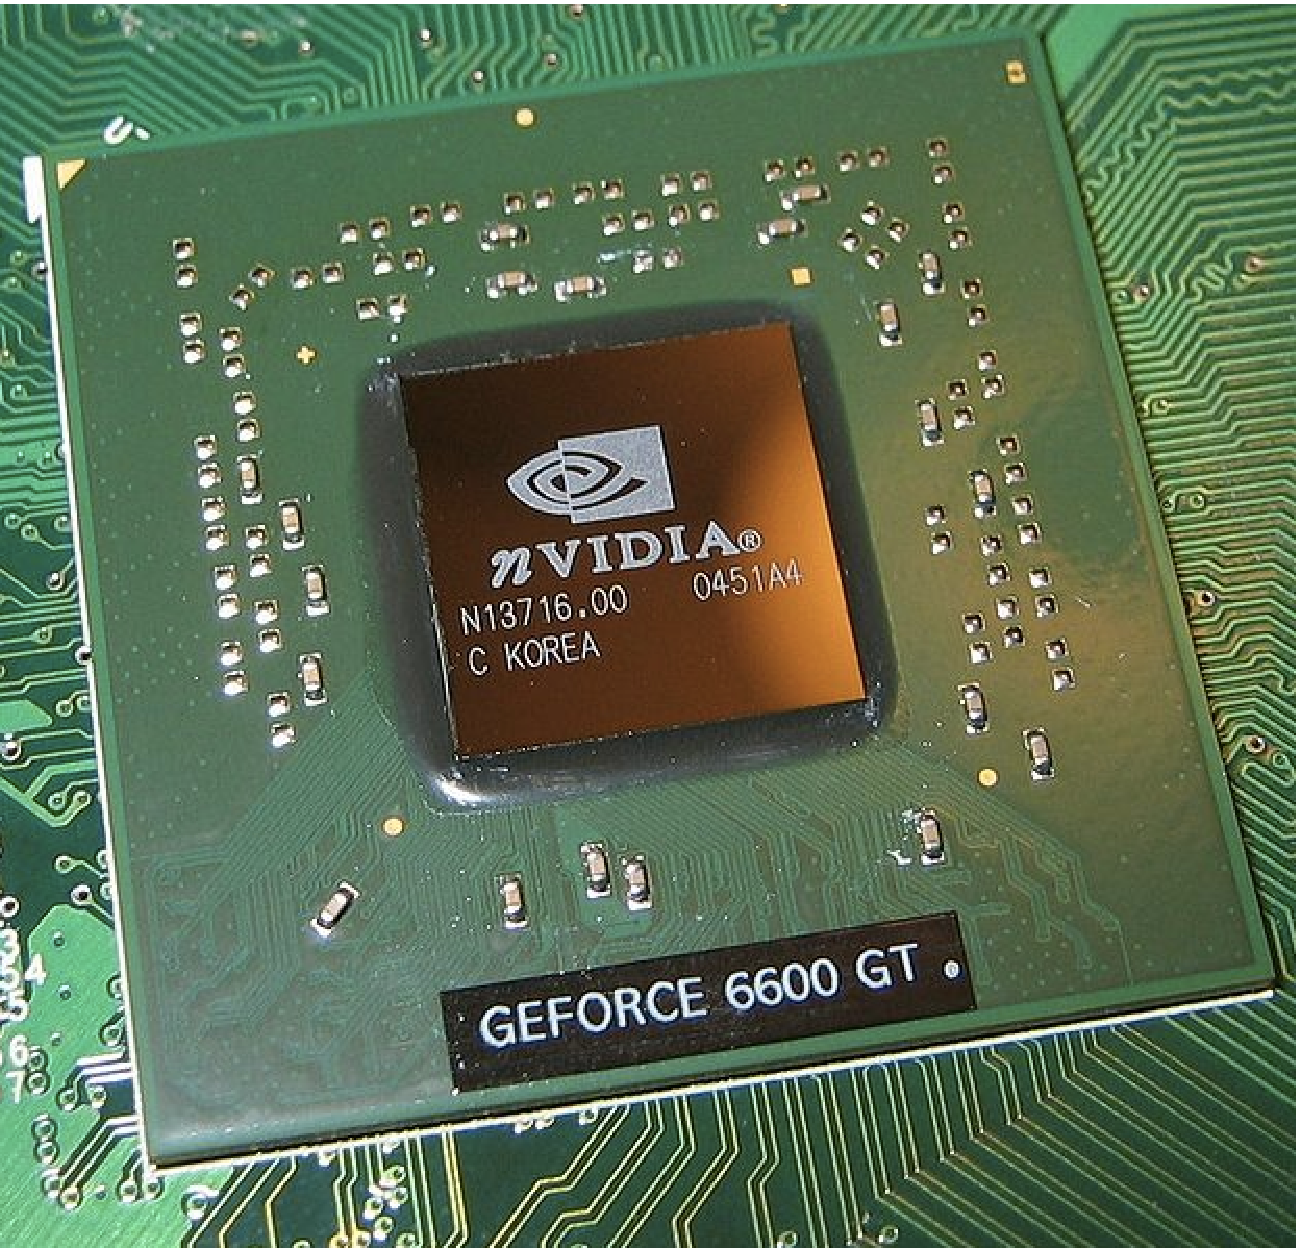
\includegraphics[scale = .175]{../../fig/gpu1} $\quad$ 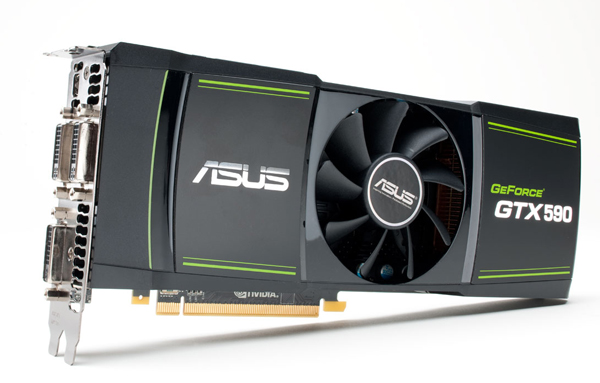
\includegraphics[scale = .175]{../../fig/gpu2}
\end{center}

\end{frame}


\begin{frame}
\frametitle{CPU / GPU cooperation}

\begin{itemize}
\item The CPU (``host") is in charge.
\uncover<2->{\item The CPU sends computationally intensive instruction sets to the GPU (``device") just like a human uses a pocket calculator.}
\end{itemize}

\begin{center}
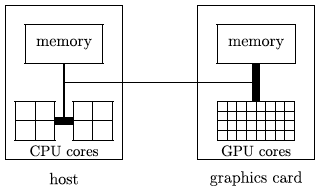
\includegraphics[scale=.8]{../../fig/communication.png}
\end{center}
\end{frame}

\begin{frame}
\frametitle{More on parallelism}
\begin{itemize}
\item {\bf Parallelism}: the practice of running multiple calculations simultaneously.
\pause \item The architecture of GPUs is extremely well-suited to massively parallel workflows.
\pause \item Note: GPU parallelism is one of many kinds of parallelism. Others include:
\begin{itemize}
\pause \item Posix threads (CPU parallelism)
\pause \item parallel cloud computing
\pause \item openMP parallelism
\pause \item openCL parallelism
\end{itemize}
\end{itemize}
\end{frame}

\begin{frame}
\frametitle{GPU parallelism speeds up calculations}
\begin{itemize}
\item Amdahl's Law says that the maximum theoretical speedup (CPU time / GPU time) is
\pause \begin{align*}
\frac{1}{1 - P + \frac{P}{N}}
\end{align*}
where:
\begin{itemize}
\item $P$ = fraction of the program's (in terms of execution time) that can be parallelized
\item $N$ = number of parallel processors
\end{itemize}
\pause \item As $N \rt \infty$, Amdahl's quantity goes to
\begin{align*}
\frac{1}{1 - P}
\end{align*}
\pause \item So if 99\% of the program can be parallelized, we could theoretically have a 100-fold speedup.
\end{itemize}
\end{frame}



\section{CUDA and our CUDA systems}

\begin{frame}
\frametitle{CUDA: making a gaming toy do science}
\begin{itemize}
 \item GPUs were originally meant to speed up graphical displays for Windows OS and video games.
 \end{itemize}
 \begin{center}

\includegraphics[scale=.19]{../../fig/nukem.png}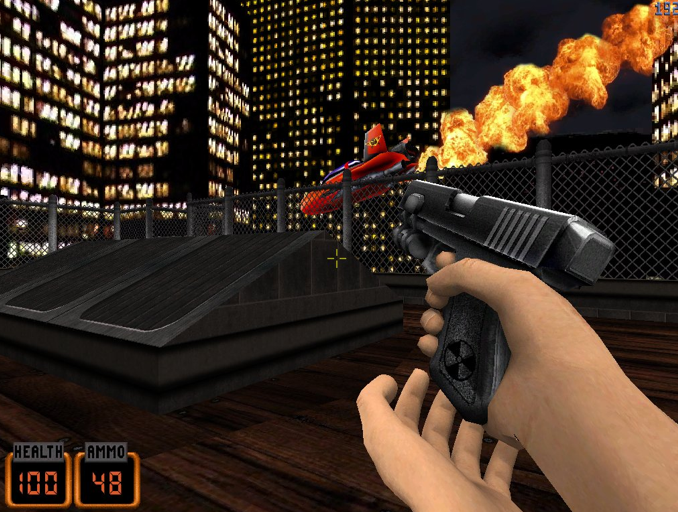
\includegraphics[scale=.19]{../../fig/nukem2.png}
\end{center}
\begin{itemize}
\pause \item {\bf CUDA}: Compute Unified Device Architecture. 
\pause \item Before CUDA, programmers could only program on GPUs using graphics languages, which are appropriate for video games but clumsy for science.
\pause \item CUDA devices support CUDA C, an extension of C for programs that use GPUs.
\end{itemize}
\end{frame}

\begin{frame}
\frametitle{CUDA-enabled servers at Iowa State}
\begin{itemize}
\item impact1.stat.iastate.edu (Red Hat Enterprise Linux Server release 6.2)
\item impact2.stat.iastate.edu (CentOS release 6.3)
\item impact3.stat.iastate.edu (Red Hat Enterprise Linux Server release 6.4)
\item impact4.stat.iastate.edu (CentOS release 6.4)
\end{itemize}
\end{frame}


\begin{frame}[fragile]
\frametitle{Specs of our CUDA systems}
\begin{itemize}
\item No graphical user interface or remote desktop capabilities. (Use the Linux command line.)
\pause \item 24 CPUs and 4 Tesla M2070 GPUs, where each GPU has 448 cores.:
\pause \item For more specs, log into impact1, 2, or 3 and enter into the command line:
\begin{lstlisting}
cd /usr/local/NVIDIA_GPU_Computing_SDK/C/bin/linux/release
./deviceQuery
\end{lstlisting}
\end{itemize}
\end{frame}

\begin{frame}[fragile]
\frametitle{Logging in}
\small 

\begin{itemize}
\item Open a command line program (Terminal in Linux and Mac OS, Cygwin or MinGW in Windows).
\pause \item Enter:
\begin{lstlisting}
ssh -p 323 ISU_ID@impact1.stat.iastate.edu
\end{lstlisting}
\pause \item Note: in general, the port number for {\tt ssh} is not always 323.
\pause \item Refer to \url{http://www.tuxfiles.org/linuxhelp/cli.html} or contact me at landau@iastate.edu for help with the Linux command line.
\pause \item Contact Stat IT at statit@iastate.edu or me if:
\begin{itemize}
\pause \item You can't log on, or
\pause \item You want to be able to log on without entering your password every time, or
\pause \item You want to shorten {\tt ssh -p 323 ISU\_ID@impact1.stat.iastate.edu} into a more manageable alias on your local machine.
\end{itemize}
\end{itemize}
\end{frame}

\begin{frame}
\frametitle{Other resources for Linux command line tools and the Linux filesystem} \small
\begin{itemize}
\item http://www.makeuseof.com/tag/an-introduction-to-the-linux-command- line/
\item http://www.freesoftwaremagazine.com/articles/command line intro
\item http://tldp.org/LDP/intro-linux/html/
\item http://tldp.org/LDP/intro-linux/html/sect 03 01.html
\item http://linux.die.net/Intro-Linux/chap 03.html
\item http://linux.about.com/od/itl guide/a/gdeitl28t02.htm
\end{itemize}
\end{frame}

\begin{frame}
\frametitle{Important directories} \small
\begin{itemize}
\item {\bf /home/ISU\_ID} Your private home folder on SMB (the collective storage system for all the stat dept linux servers). Files in here are stored remotely on SMB, not locally on impact1-3.
\pause \item {\bf /Cyfiles/ISU\_ID} Your private Cyfiles folder. Files in here are stored remotely on the Cyfiles server, not locally on impact1-3.
\pause \item {\bf /tmp} 
\begin{itemize}
\item Everything in here is stored locally on impact1, etc., wherever you're logged in.  
\pause \item To avoid communicating over a network when you want fast computation, put large datasets here.
\pause \item Note: {\bf /tmp} automatically empties periodically.
\end{itemize}
\pause \item {\bf /usr/local/NVIDIA\_GPU\_Computing\_SDK}
\begin{itemize}
\item Example CUDA C code. Stored locally on impact1, etc.
\pause \item You do not have write privileges here.
\end{itemize}
\end{itemize}
\end{frame}


\section{GPU computing with R}


\begin{frame}
\frametitle{GPU-enabled R packages}
\begin{itemize}
\item {\tt WideLM} - used to quickly fit a large number of linear models to a fixed design matrix and response vector.
\pause \item {\tt magma} - a small linear algebra with implementations of backsolving and the LU factorization.
\pause \item {\tt cudaBayesreg} - implements a Bayesian model for fitting fMRI data.
\pause \item  {\tt gcbd} - a Debian package for �benchmarking� linear algebra algorithms such as the QR, SVD and LU.factorizations.
\pause \item {\tt gputools} - probably the most useful of these 5.
\end{itemize}
\end{frame}



\begin{frame}
\frametitle{Contents of {\tt gputools}}


\begin{itemize}
\item Choose your device:

\begin{center}
\begin{tabular}{r|l|c}
 \bf gputools function & \bf CPU analog  & \bf Same usage? \\ \hline
chooseGpu() & none & NA \\
getGpuId() & none & NA
\end{tabular}
\end{center}

\pause \item Linear algebra: 
\begin{center}
\begin{tabular}{r|l|c}

 \bf gputools function & \bf CPU analog  & \bf Same usage? \\ \hline
gpuDist() & dist() & no \\ 
gpuMatMult() & \%*\% operator & no \\ 
gpuCrossprod() & crossprod() & yes \\ 
gpuTcrossprod() & tcrossprod() & yes \\ 
gpuQr() & qr() & almost \\ 
gpuSolve() & solve() & no \\ 
gpuSvd() & svd() & almost \\ 
\end{tabular}
\end{center}
\end{itemize}
\end{frame}


\begin{frame}
\begin{itemize}
\item Simple model fitting: 
\begin{center}
\begin{tabular}{r|l|c}

 \bf gputools function & \bf CPU analog  & \bf Same usage? \\ \hline
gpuLm() & lm() & yes \\ 
gpuLsfit() & lsfit() & yes \\ 
gpuGlm() & glm() & yes \\
gpuGlm.fit() & glm.fit() & yes \\ 
\end{tabular} $\quad$ \newline
\end{center}

\pause \item Hypothesis testing: 

\begin{center}
\begin{tabular}{r|l|c}
 \bf gputools function & \bf CPU analog  & \bf Same usage? \\ \hline
gpuTtest() & t.test() & no \\ 
getAucEstimate() & ??? & ??? \\
\end{tabular} $\quad$ \newline
\end{center}
\end{itemize}
\end{frame}



\begin{frame}
\begin{itemize}
\item Other routines: \scriptsize
\begin{center}
\begin{tabular}{r|l|c}
\bf gputools function & \bf CPU analog  & \bf Same usage? \\ \hline
gpuHclust() & hclust() & no \\
gpuDistClust() & hclust(dist()) & no \\ 
gpuFastICA() & fastICA() (fastICA package) & yes \\
gpuGranger() & grangertest() (lmtest package) & no \\
gpuMi() & ??? & ??? \\
gpuSvmPredict() & www.jstatsoft.org/v15/i09/paper & no \\
gpuSvmTrain() & www.jstatsoft.org/v15/i09/paper & no \\
\end{tabular}
\end{center}
\end{itemize}
\end{frame}




\begin{frame}[fragile]
\frametitle{Example}

\lstset{basicstyle=\footnotesize}
\begin{lstlisting}
> getGpuID()
[1] 0
> chooseGpu(3)
[[1]]
[1] 3
> getGpuID()
[1] 3
> A <- matrix(runif(1e7), nrow = 1e4)
> B <- matrix(runif(1e7), nrow = 1e4)
> ptm <- proc.time(); C <- gpuMatMult(A, B); 
> proc.time() - ptm
   user   system  elapsed
   2.959  2.190     5.159
> ptm <-  proc.time(); C <- A % * % B; 
> proc.time() - ptm
   user   system  elapsed
   116.389  0.166   116.503
\end{lstlisting}
\end{frame}
\lstset{basicstyle=\tiny}

\begin{frame}
\frametitle{Speedup}
\begin{center}
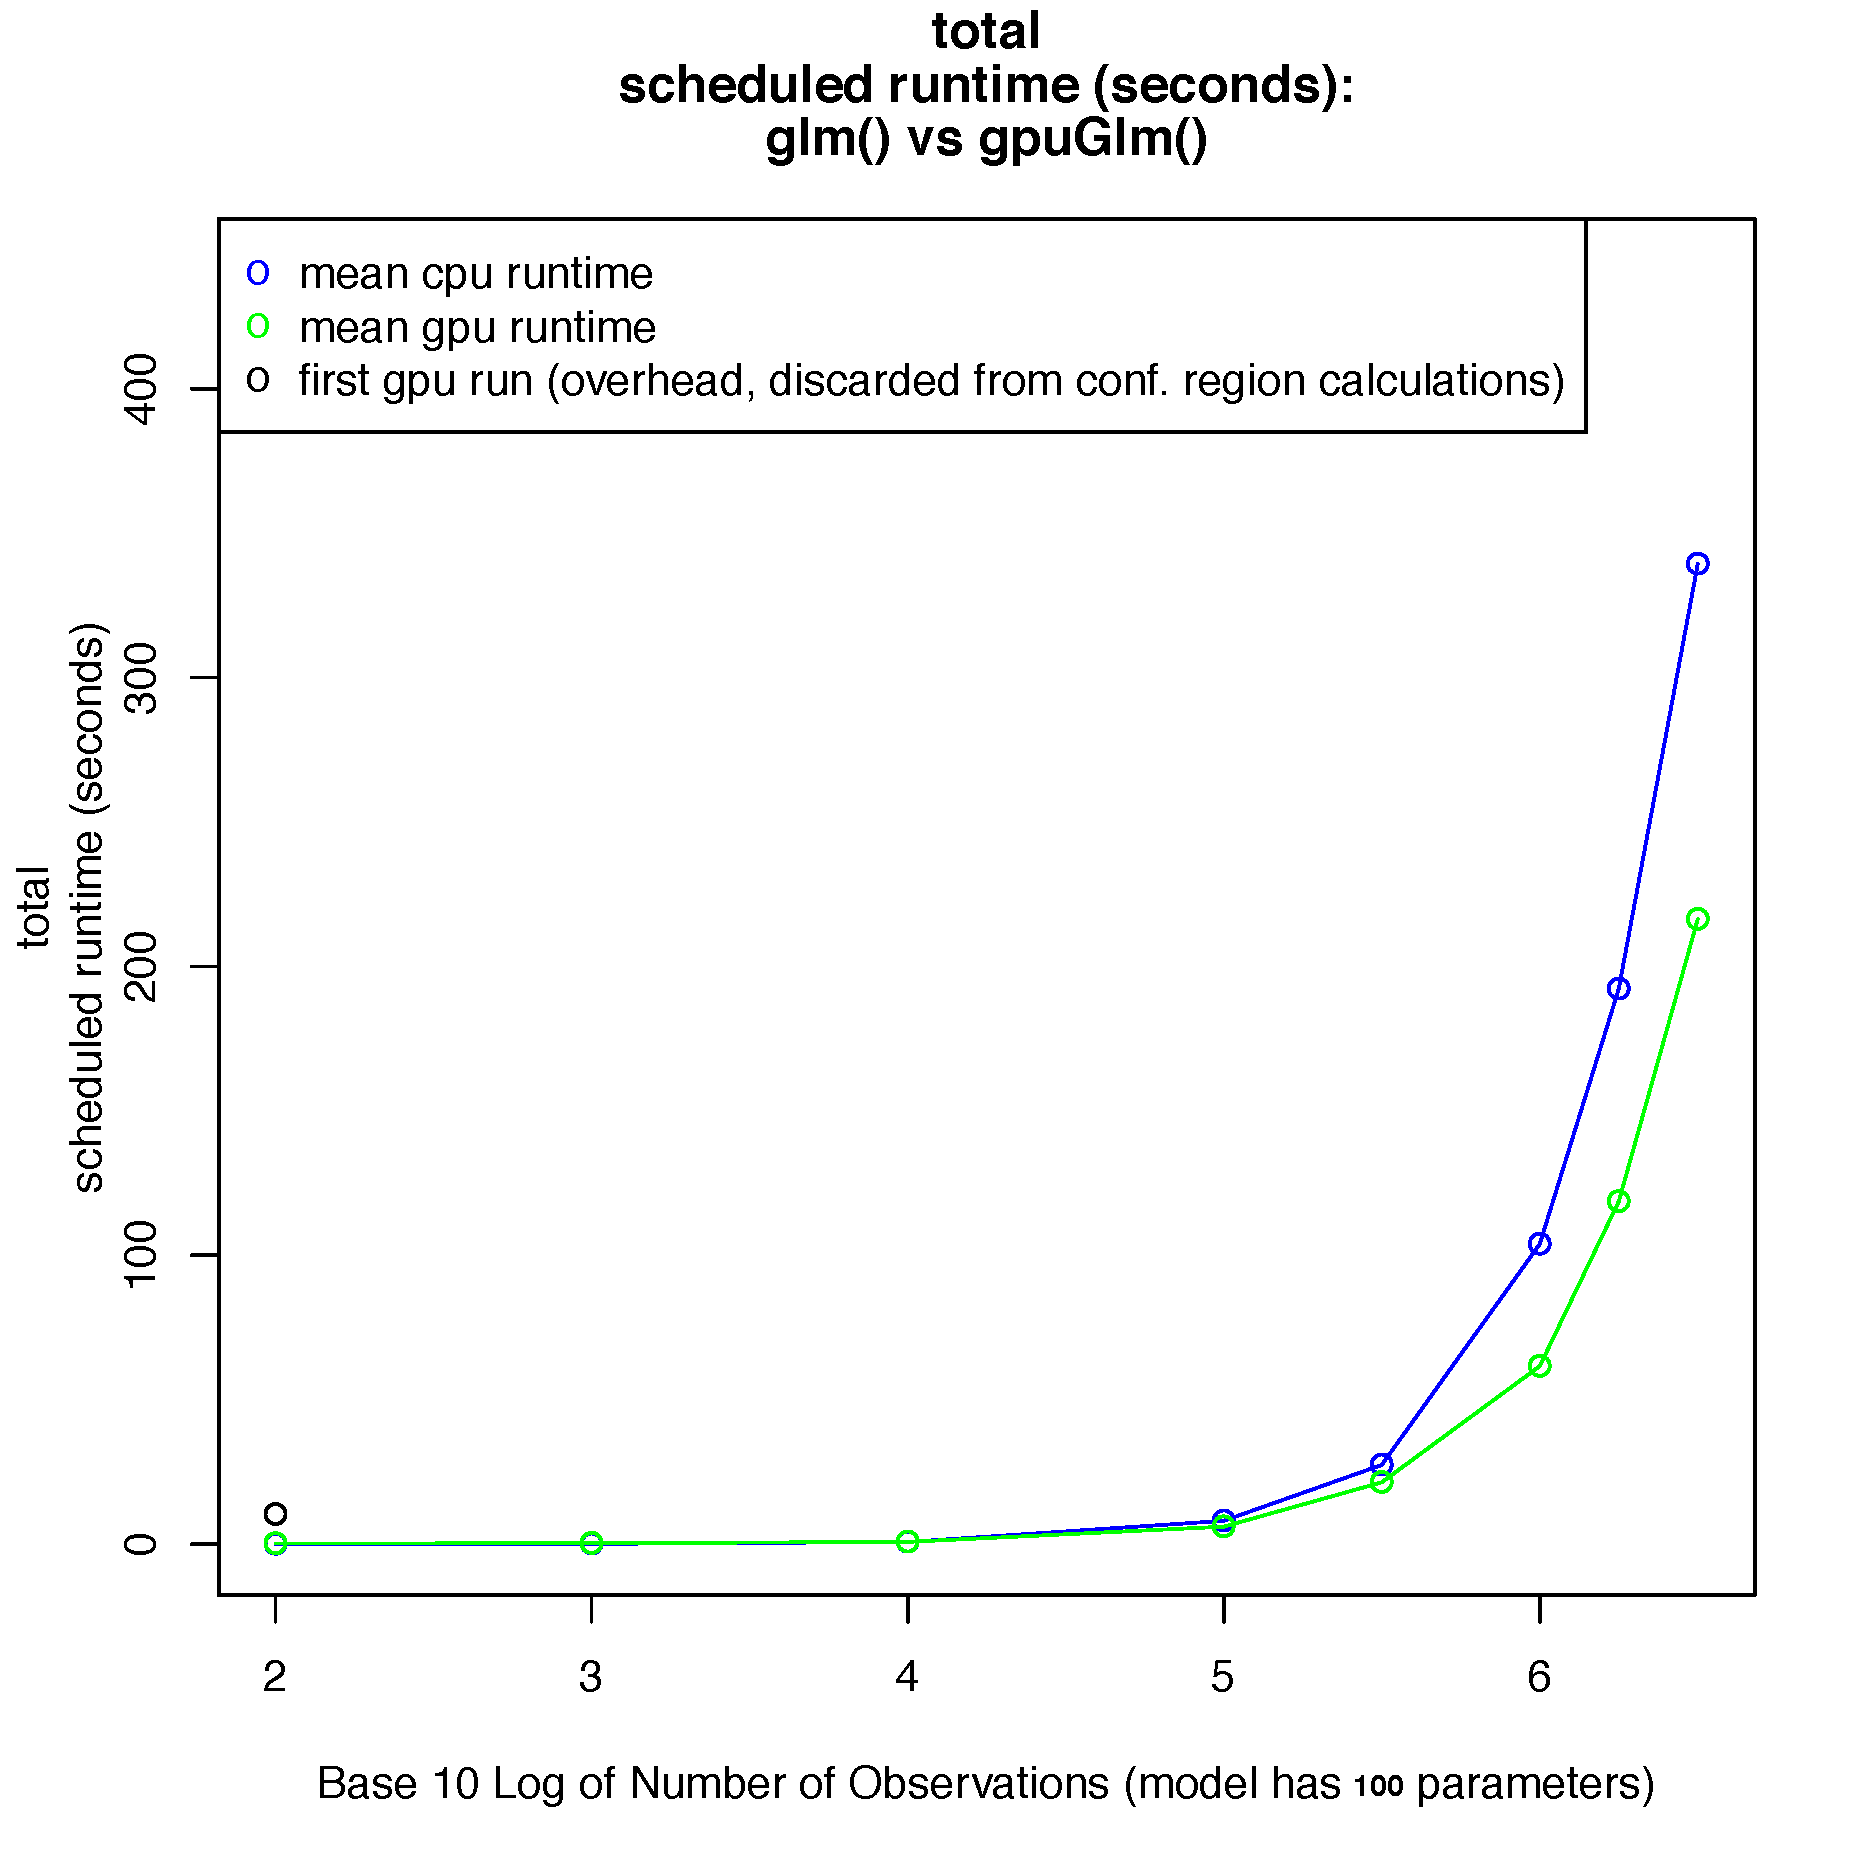
\includegraphics[scale=.25]{../../fig/gpuglm}
\end{center}
\end{frame}


\begin{frame}
\frametitle{Speedup}
\begin{center}
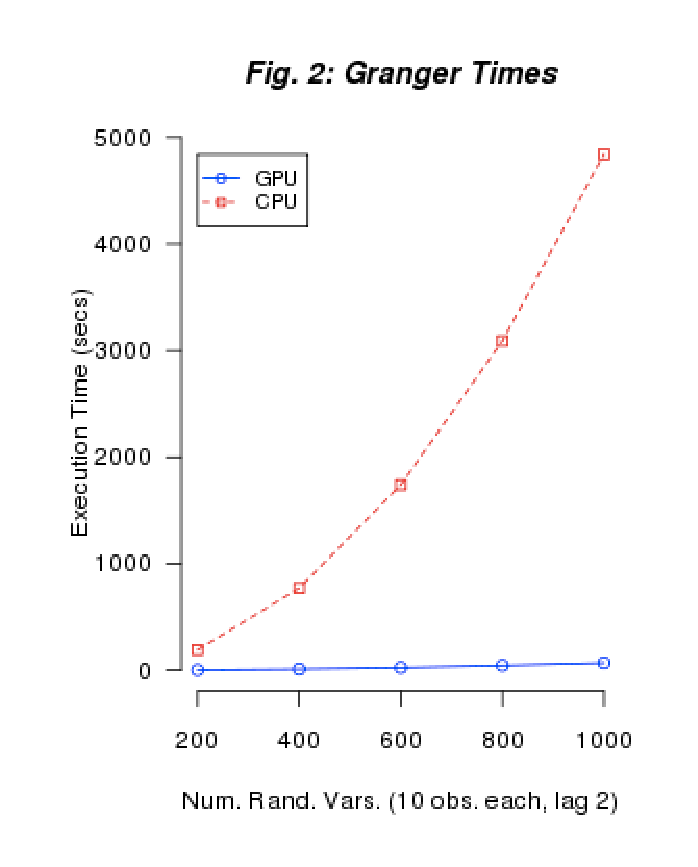
\includegraphics[scale=.55]{../../fig/granger}
\end{center}
\end{frame}

\begin{frame}
\frametitle{Tentative syllabus for the series}

\small
\begin{enumerate}
\item Intro and {\tt gputools}
\pause \item A codeless intro to GPU parallelism
\pause \item Intro to CUDA C
\pause \item CUDA C: K-means and MCMC
\pause \item CUDA C: Shared memory and performance measurement
\pause \item CUDA C: Race conditions, atomics, and warps
\pause \item CUBLAS and CULA: linear algebra libraries for CUDA C
\pause \item CURAND: a GPU-enabled library for fast random number generation
\pause \item Thrust: the GPU analog of the C++ Standard Template Library
\pause \item Intro to Python: preparation for PyCUDA
\pause \item PyCUDA: a Python module for GPU computing
\end{enumerate}
\end{frame}



\section{How GPU parallelism works}

\begin{frame}
\frametitle{How GPU parallelism works} \scriptsize
\begin{enumerate}
\scriptsize
\item The CPU sends a command called a {\bf kernel} to a GPU.
\pause \item The GPU executes several duplicate realizations of this command, called {\bf threads}.
\begin{itemize}
\scriptsize
\pause \item These threads are grouped into bunches called {\bf blocks}.
\pause \item The sum total of all threads in a kernel is called a {\bf grid}.
\end{itemize}
\end{enumerate}

\begin{itemize}
\scriptsize
\item Toy example:
\begin{itemize}
\scriptsize
\item CPU says something like, ``Hey, GPU. Sum pairs of adjacent numbers. Use the array, (1, 2, 3, 4, 5, 6, 7, 8). Use 2 blocks of 2 threads each."
\pause \item GPU thinks: ``Sum pairs of adjacent numbers" is a kernel that I need to apply to the array, (1, 2, 3, 4, 5, 6, 8).
\pause \item The GPU spawns 2 blocks, each with 2 threads:
\end{itemize}
\end{itemize}

\pause \begin{center}
\begin{tabular}{c|cc|cc}
Block  & \multicolumn{2}{c|}{0} &  \multicolumn{2}{c}{1} \\ \hline
Thread & 0 & 1 & 0 & 1  \\ \hline
Action & 1 + 2 & 3 + 4 & 5 + 6 & 7 + 8 \\
\end{tabular}
\end{center}

\begin{itemize}
\scriptsize
\pause \item All four actions above happen simultaneously.
\pause \item I could have also used 1 block with 4 threads and given the threads different pairs of numbers.
\end{itemize}
\end{frame}

\begin{frame}
\begin{center}
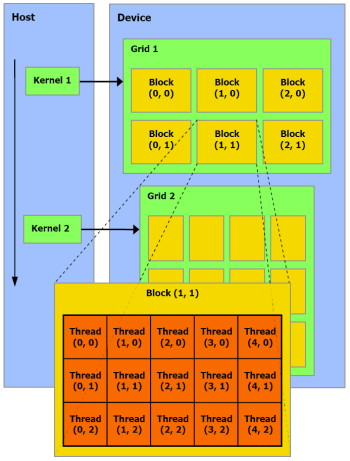
\includegraphics[scale=.7]{../../fig/gridBlocksThreads.jpg}
\end{center}
\end{frame}


\section{Examples}

\subsection{Vector addition}

\begin{frame}
\frametitle{Vector addition}


\begin{itemize}
\item Say I have 2 vectors,


\begin{align*}
a = \begin{bmatrix} a_1 \\ a_2 \\ \vdots \\ a_n \end{bmatrix} \qquad b = \begin{bmatrix} b_1 \\ b_2 \\ \vdots \\ b_n  \end{bmatrix}
\end{align*}

\pause \item I want to compute their component-wise sum,
\begin{align*}
c = \begin{bmatrix} c_1 \\ c_2 \\ \vdots \\ c_n \end{bmatrix} = \begin{bmatrix} a_1 + b_1 \\ a_2 + b_2 \\ \vdots \\ a_n + b_n  \end{bmatrix}
\end{align*}

\end{itemize}
\end{frame}

\begin{frame}
\frametitle{Vector addition}
\begin{center}
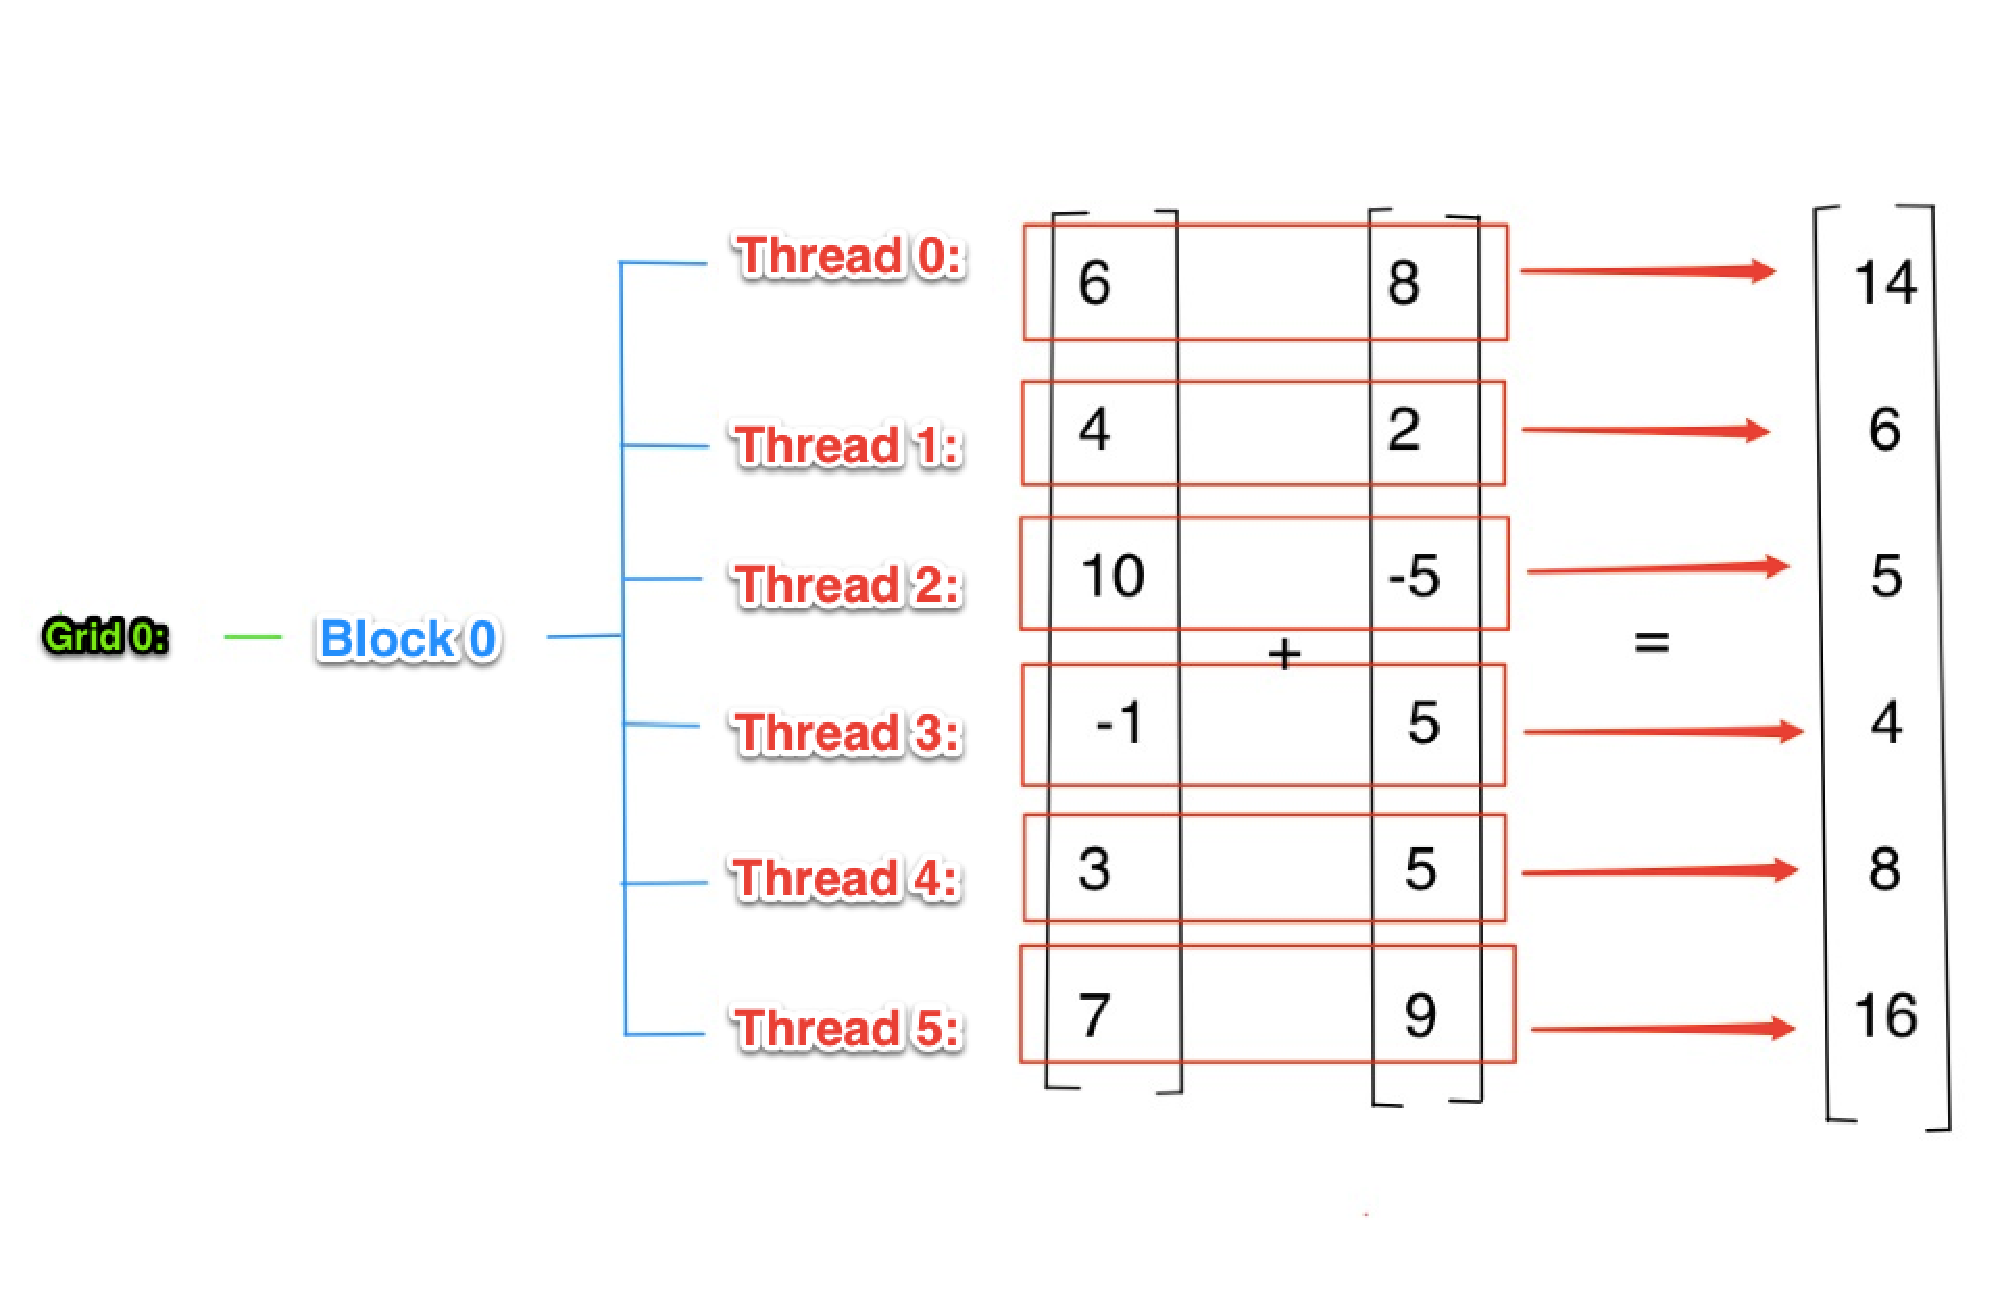
\includegraphics[scale=.25]{../../fig/vadd1.pdf}
\end{center}
\end{frame}


\begin{frame}
\frametitle{Vector addition}
\begin{center}
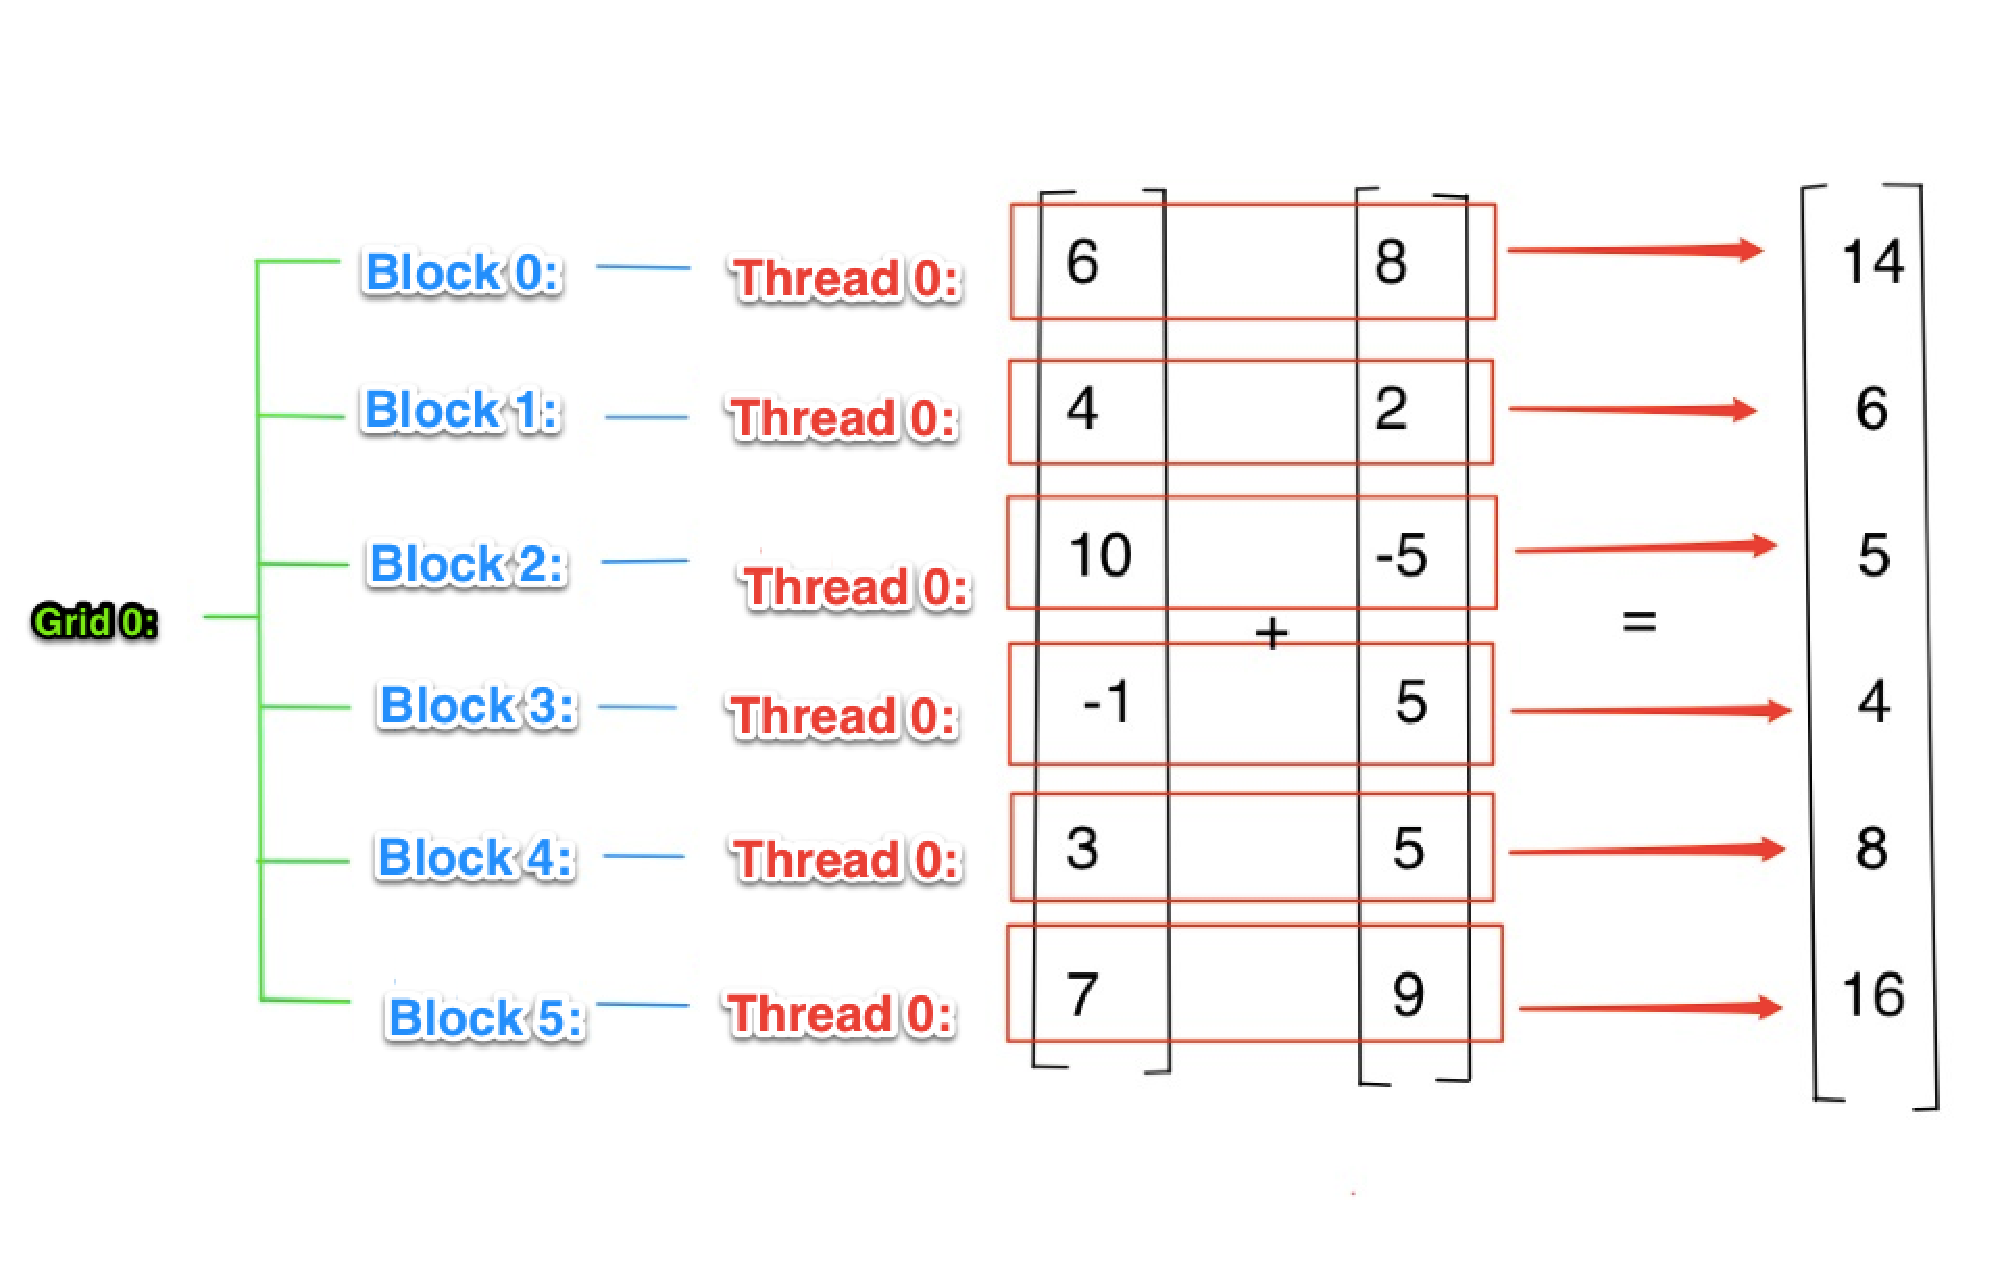
\includegraphics[scale=.25]{../../fig/vadd2.pdf}
\end{center}
\end{frame}

\begin{frame}
\frametitle{Vector addition}
\begin{center}
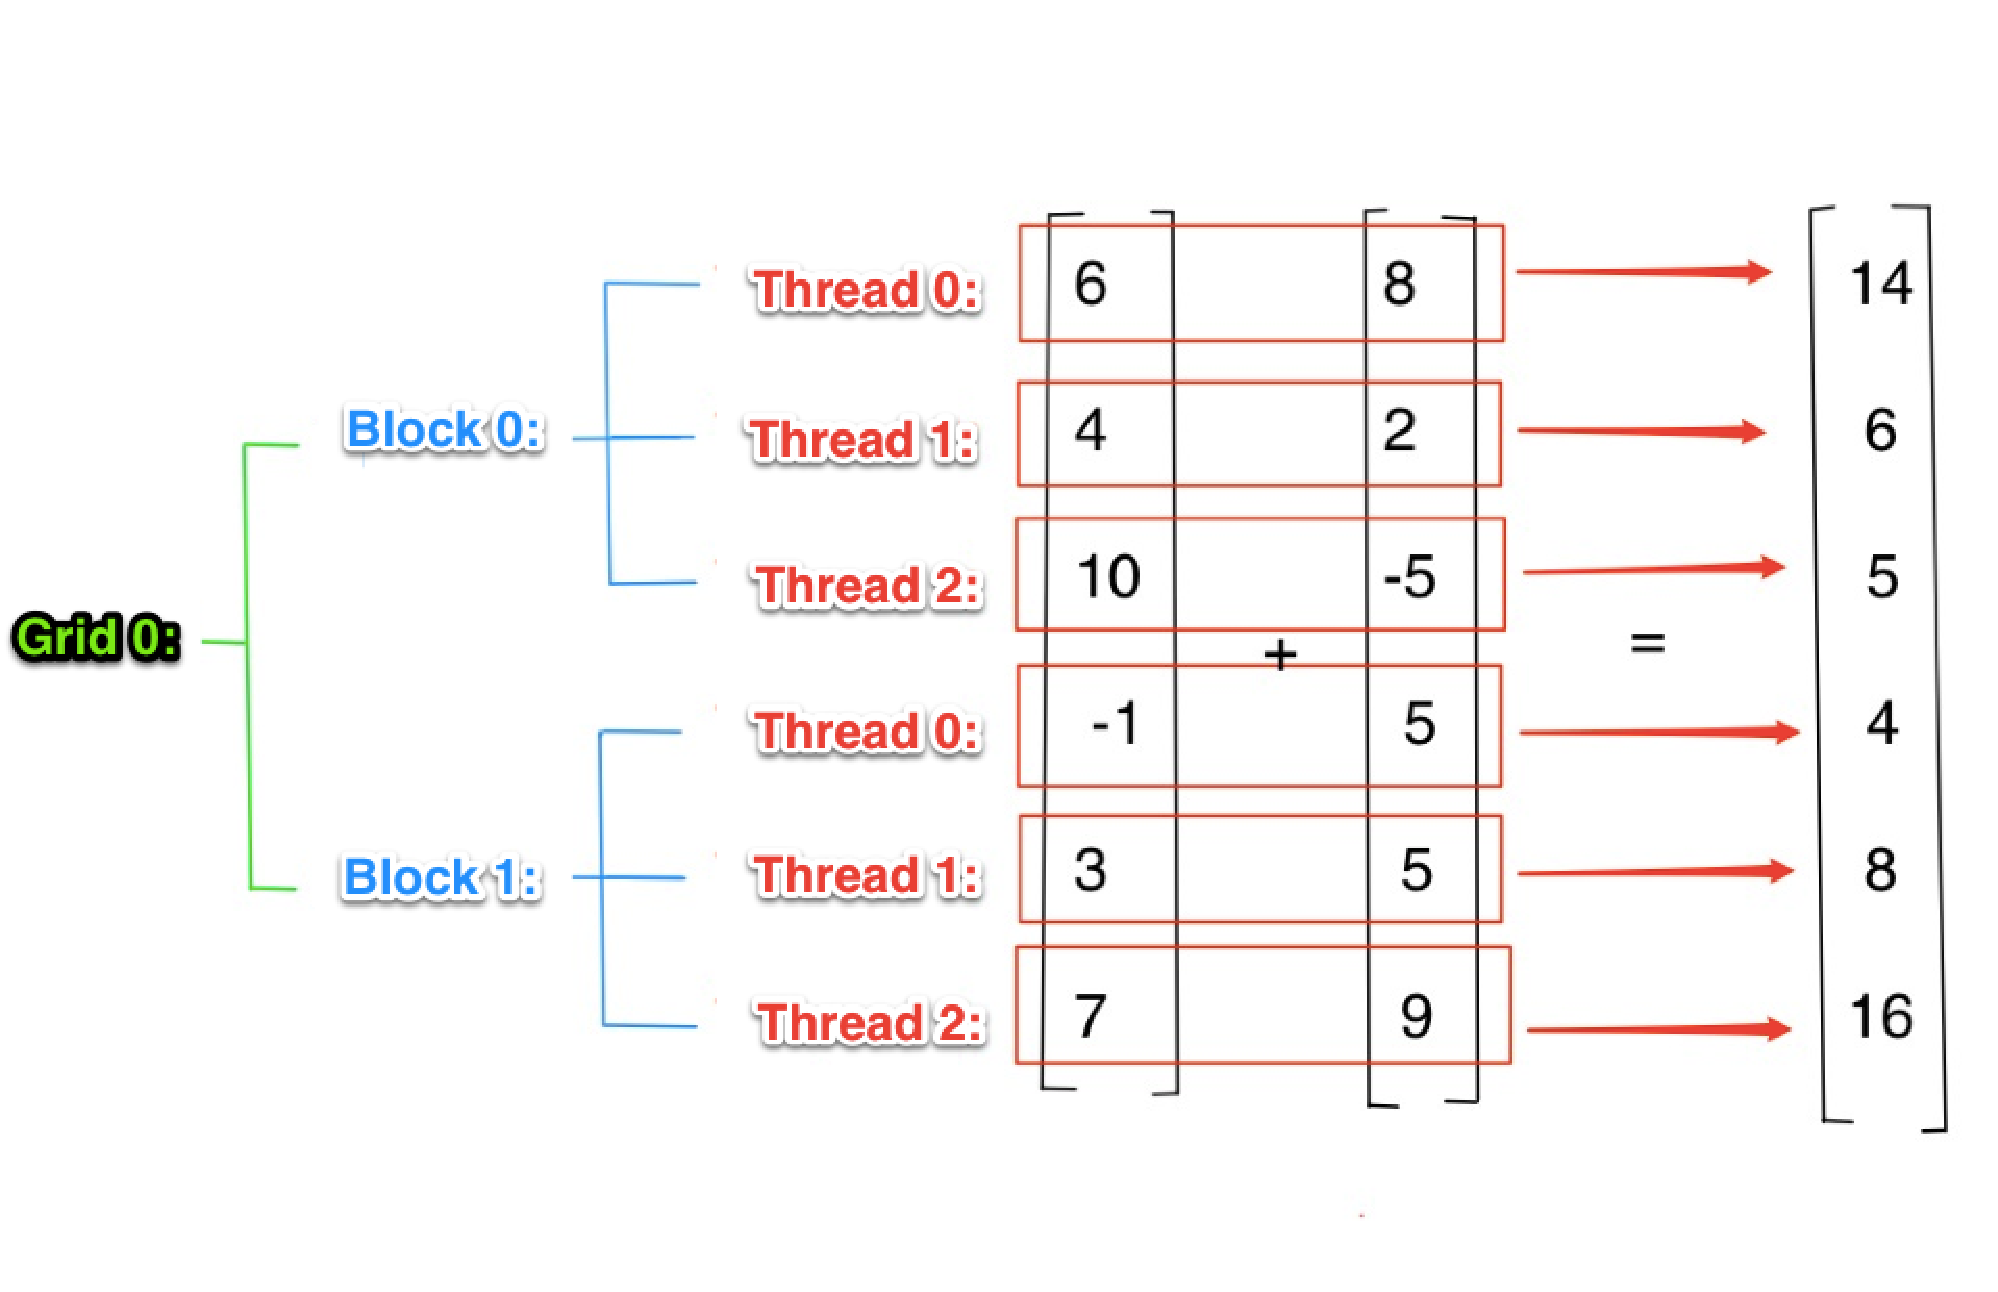
\includegraphics[scale=.25]{../../fig/vadd3.pdf}
\end{center}
\end{frame}

\begin{frame}[fragile]
\frametitle{Vector addition: {\tt vectorsums.cu}} \lstset{basicstyle=\tiny}
\begin{lstlisting}[name=vc]
#include <stdio.h>
#include <stdlib.h>
#include <cuda.h>
#include <cuda_runtime.h> 

#define N 10

__global__ void add(int *a, int *b, int *c){
  int bid = blockIdx.x;
  if(bid < N)
    c[bid] = a[bid] + b[bid];
}

int main(void) {
  int i, a[N], b[N], c[N];
  int *dev_a, *dev_b, *dev_c;

  cudaMalloc((void**) &dev_a, N*sizeof(int));
  cudaMalloc((void**) &dev_b, N*sizeof(int));
  cudaMalloc((void**) &dev_c, N*sizeof(int));

  for(i=0; i<N; i++){
    a[i] = -i;
    b[i] = i*i;
  }
  
  cudaMemcpy(dev_a, a, N*sizeof(int), cudaMemcpyHostToDevice);
  cudaMemcpy(dev_b, b, N*sizeof(int), cudaMemcpyHostToDevice);
\end{lstlisting}
\end{frame}


\begin{frame}[fragile]
\frametitle{Vector addition: {\tt vectorsums.cu}} \lstset{basicstyle=\tiny}
\begin{lstlisting}[name=vc]
  add<<<N,1>>>(dev_a, dev_b, dev_c);

  cudaMemcpy(c, dev_c, N*sizeof(int), cudaMemcpyDeviceToHost);

  printf("\na + b = c\n");
  for(i = 0; i<N; i++){
    printf("%5d + %5d = %5d\n", a[i], b[i], c[i]);
  }

  cudaFree(dev_a);
  cudaFree(dev_b);
  cudaFree(dev_c);
}
\end{lstlisting}
\end{frame}


\begin{frame}[fragile]
\frametitle{Compiling and running {\tt vectorsums.cu}}
\begin{lstlisting}
> nvcc vectorsums.cu -o vectorsums
> ./vectorsums
a + b = c
    0 +    0 =    0
   -1 +    1 =    0
   -2 +    4 =    2
   -3 +    9 =    6
   -4 +   16 =   12
   -5 +   25 =   20
   -6 +   36 =   30
   -7 +   49 =   42
   -8 +   64 =   56
   -9 +   81 =   72
\end{lstlisting}
\end{frame}





\subsection{Pairwise sum}

\begin{frame}
\frametitle{Pairwise sum}

\begin{itemize}
\item Let's take the pairwise sum of the vector,

\begin{align*}
(5, 2, -3, 1, 1, 8, 2, 6)
\end{align*}

using 1 block of 4 threads.
\end{itemize}
\end{frame}

\begin{frame}
\frametitle{Pairwise sum}
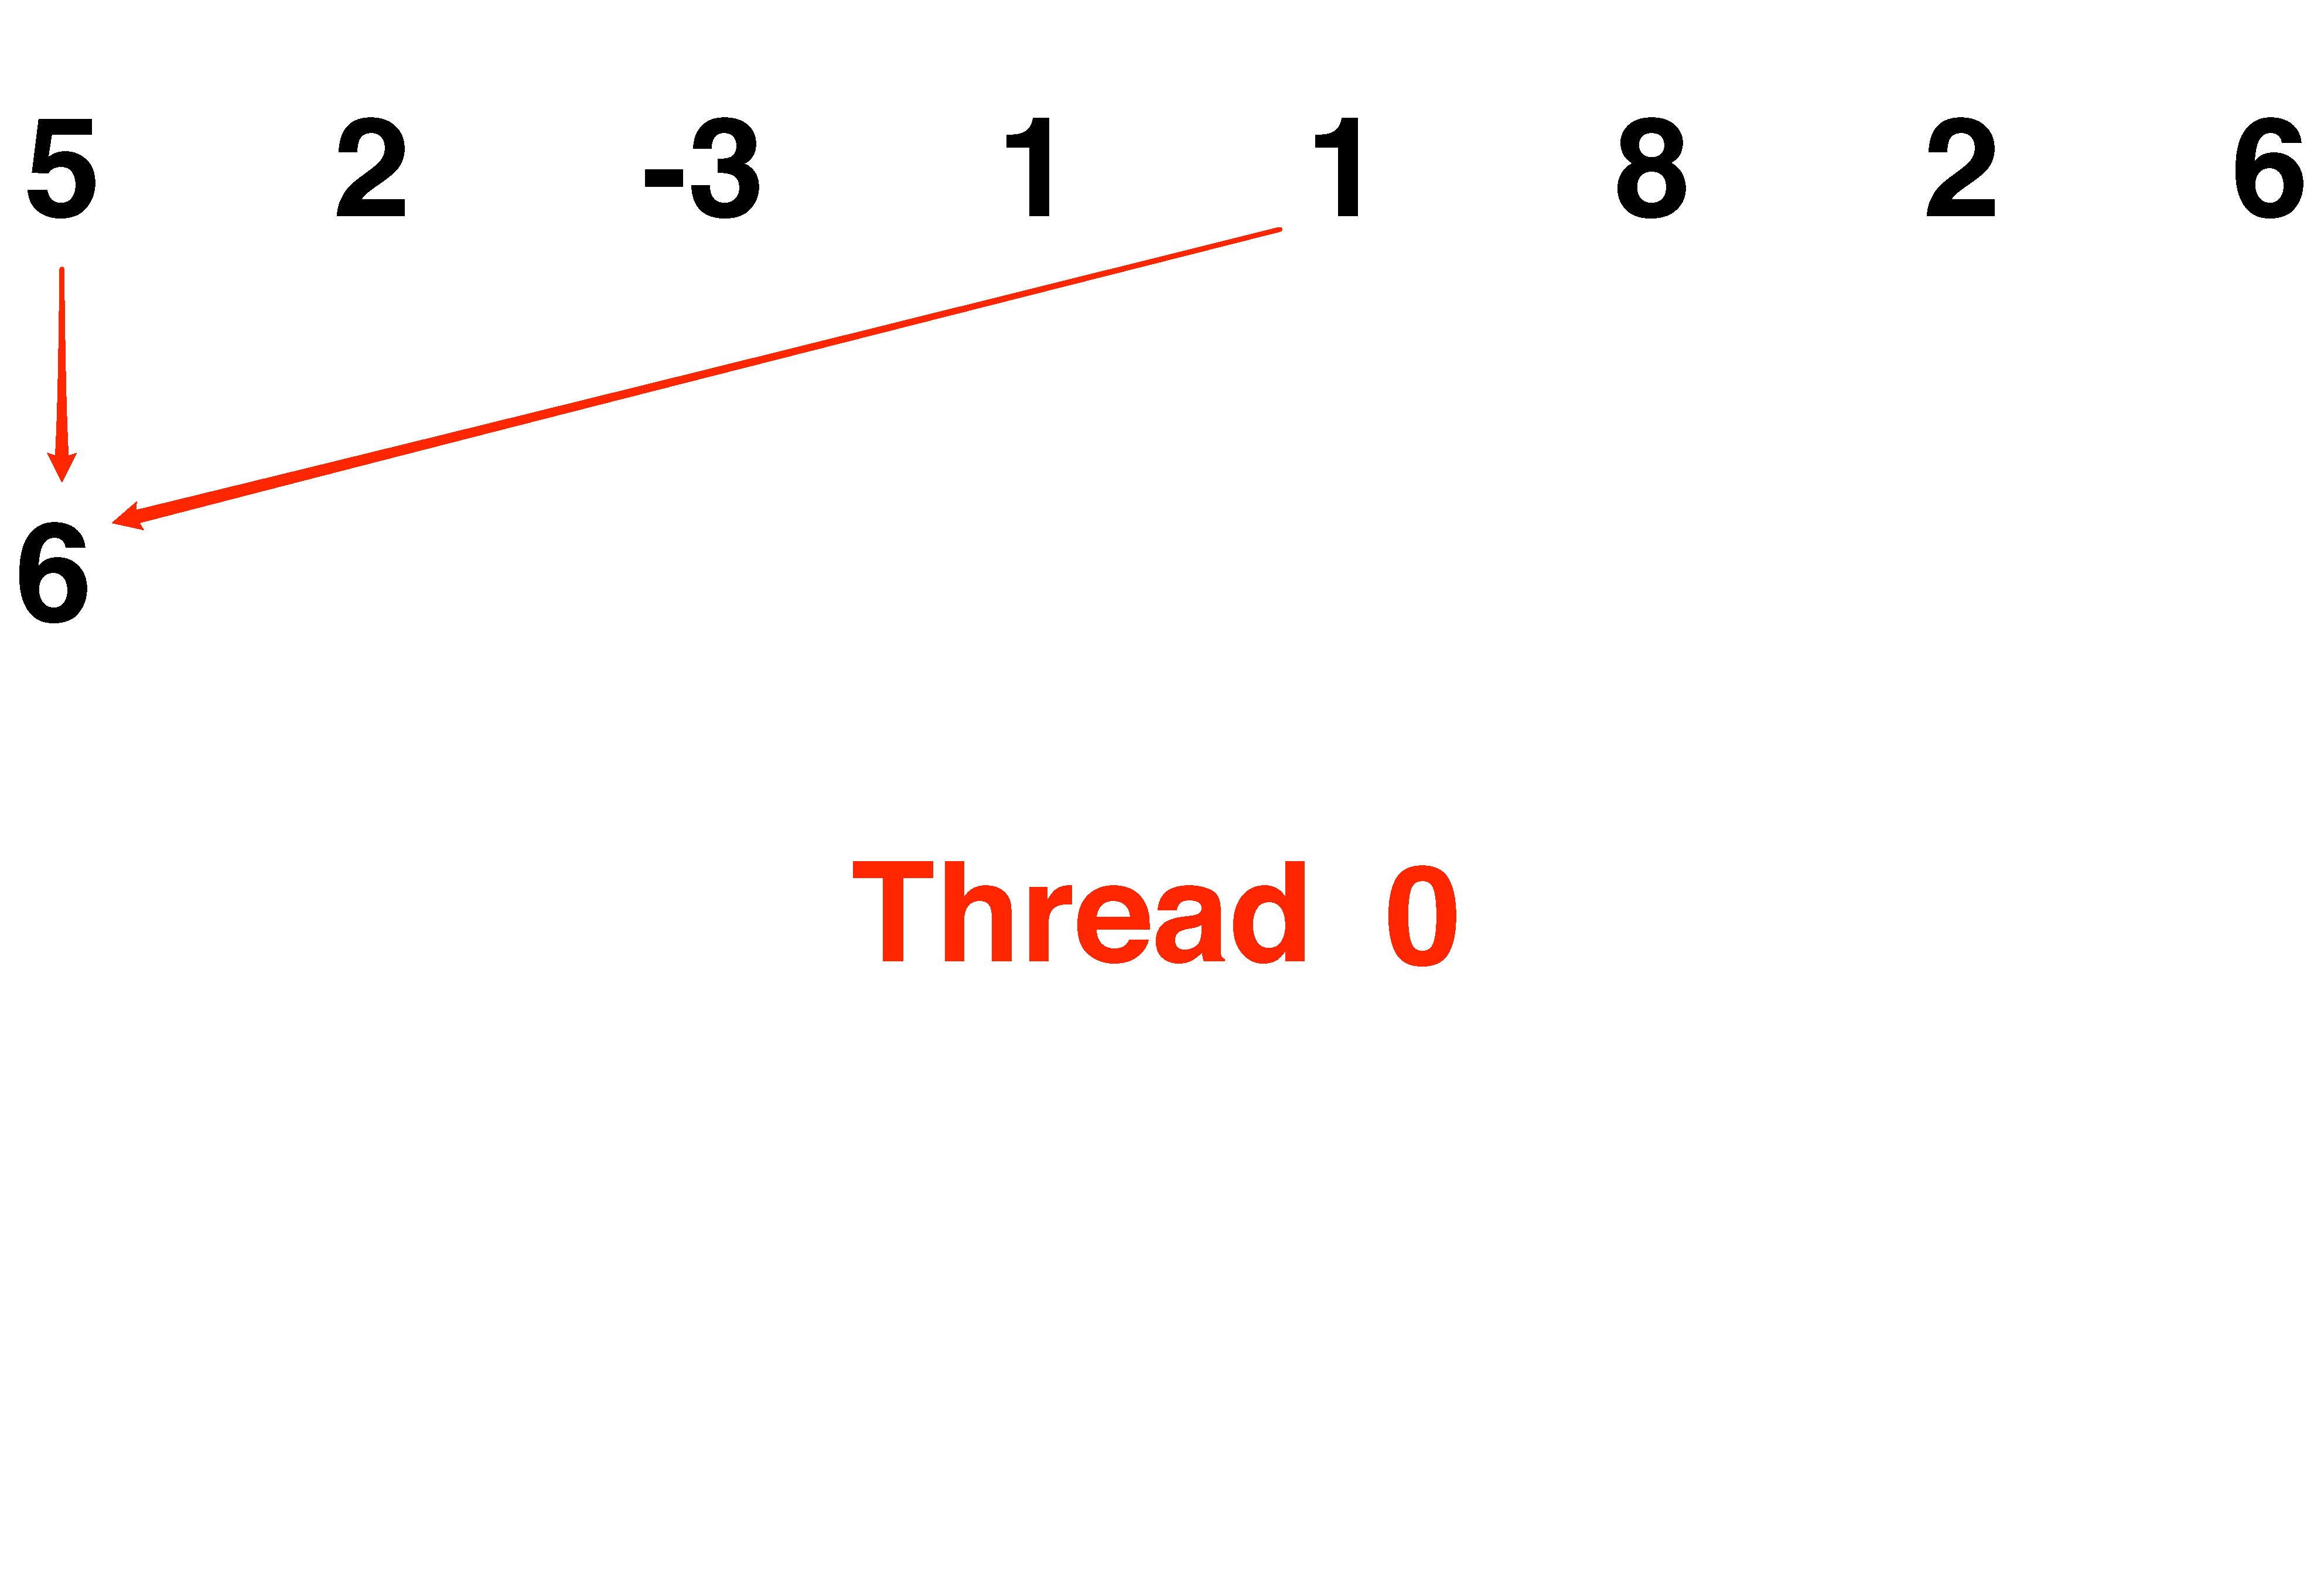
\includegraphics[scale=.15]{../../fig/psum1.pdf}
\end{frame}

\begin{frame}
\frametitle{Pairwise sum}
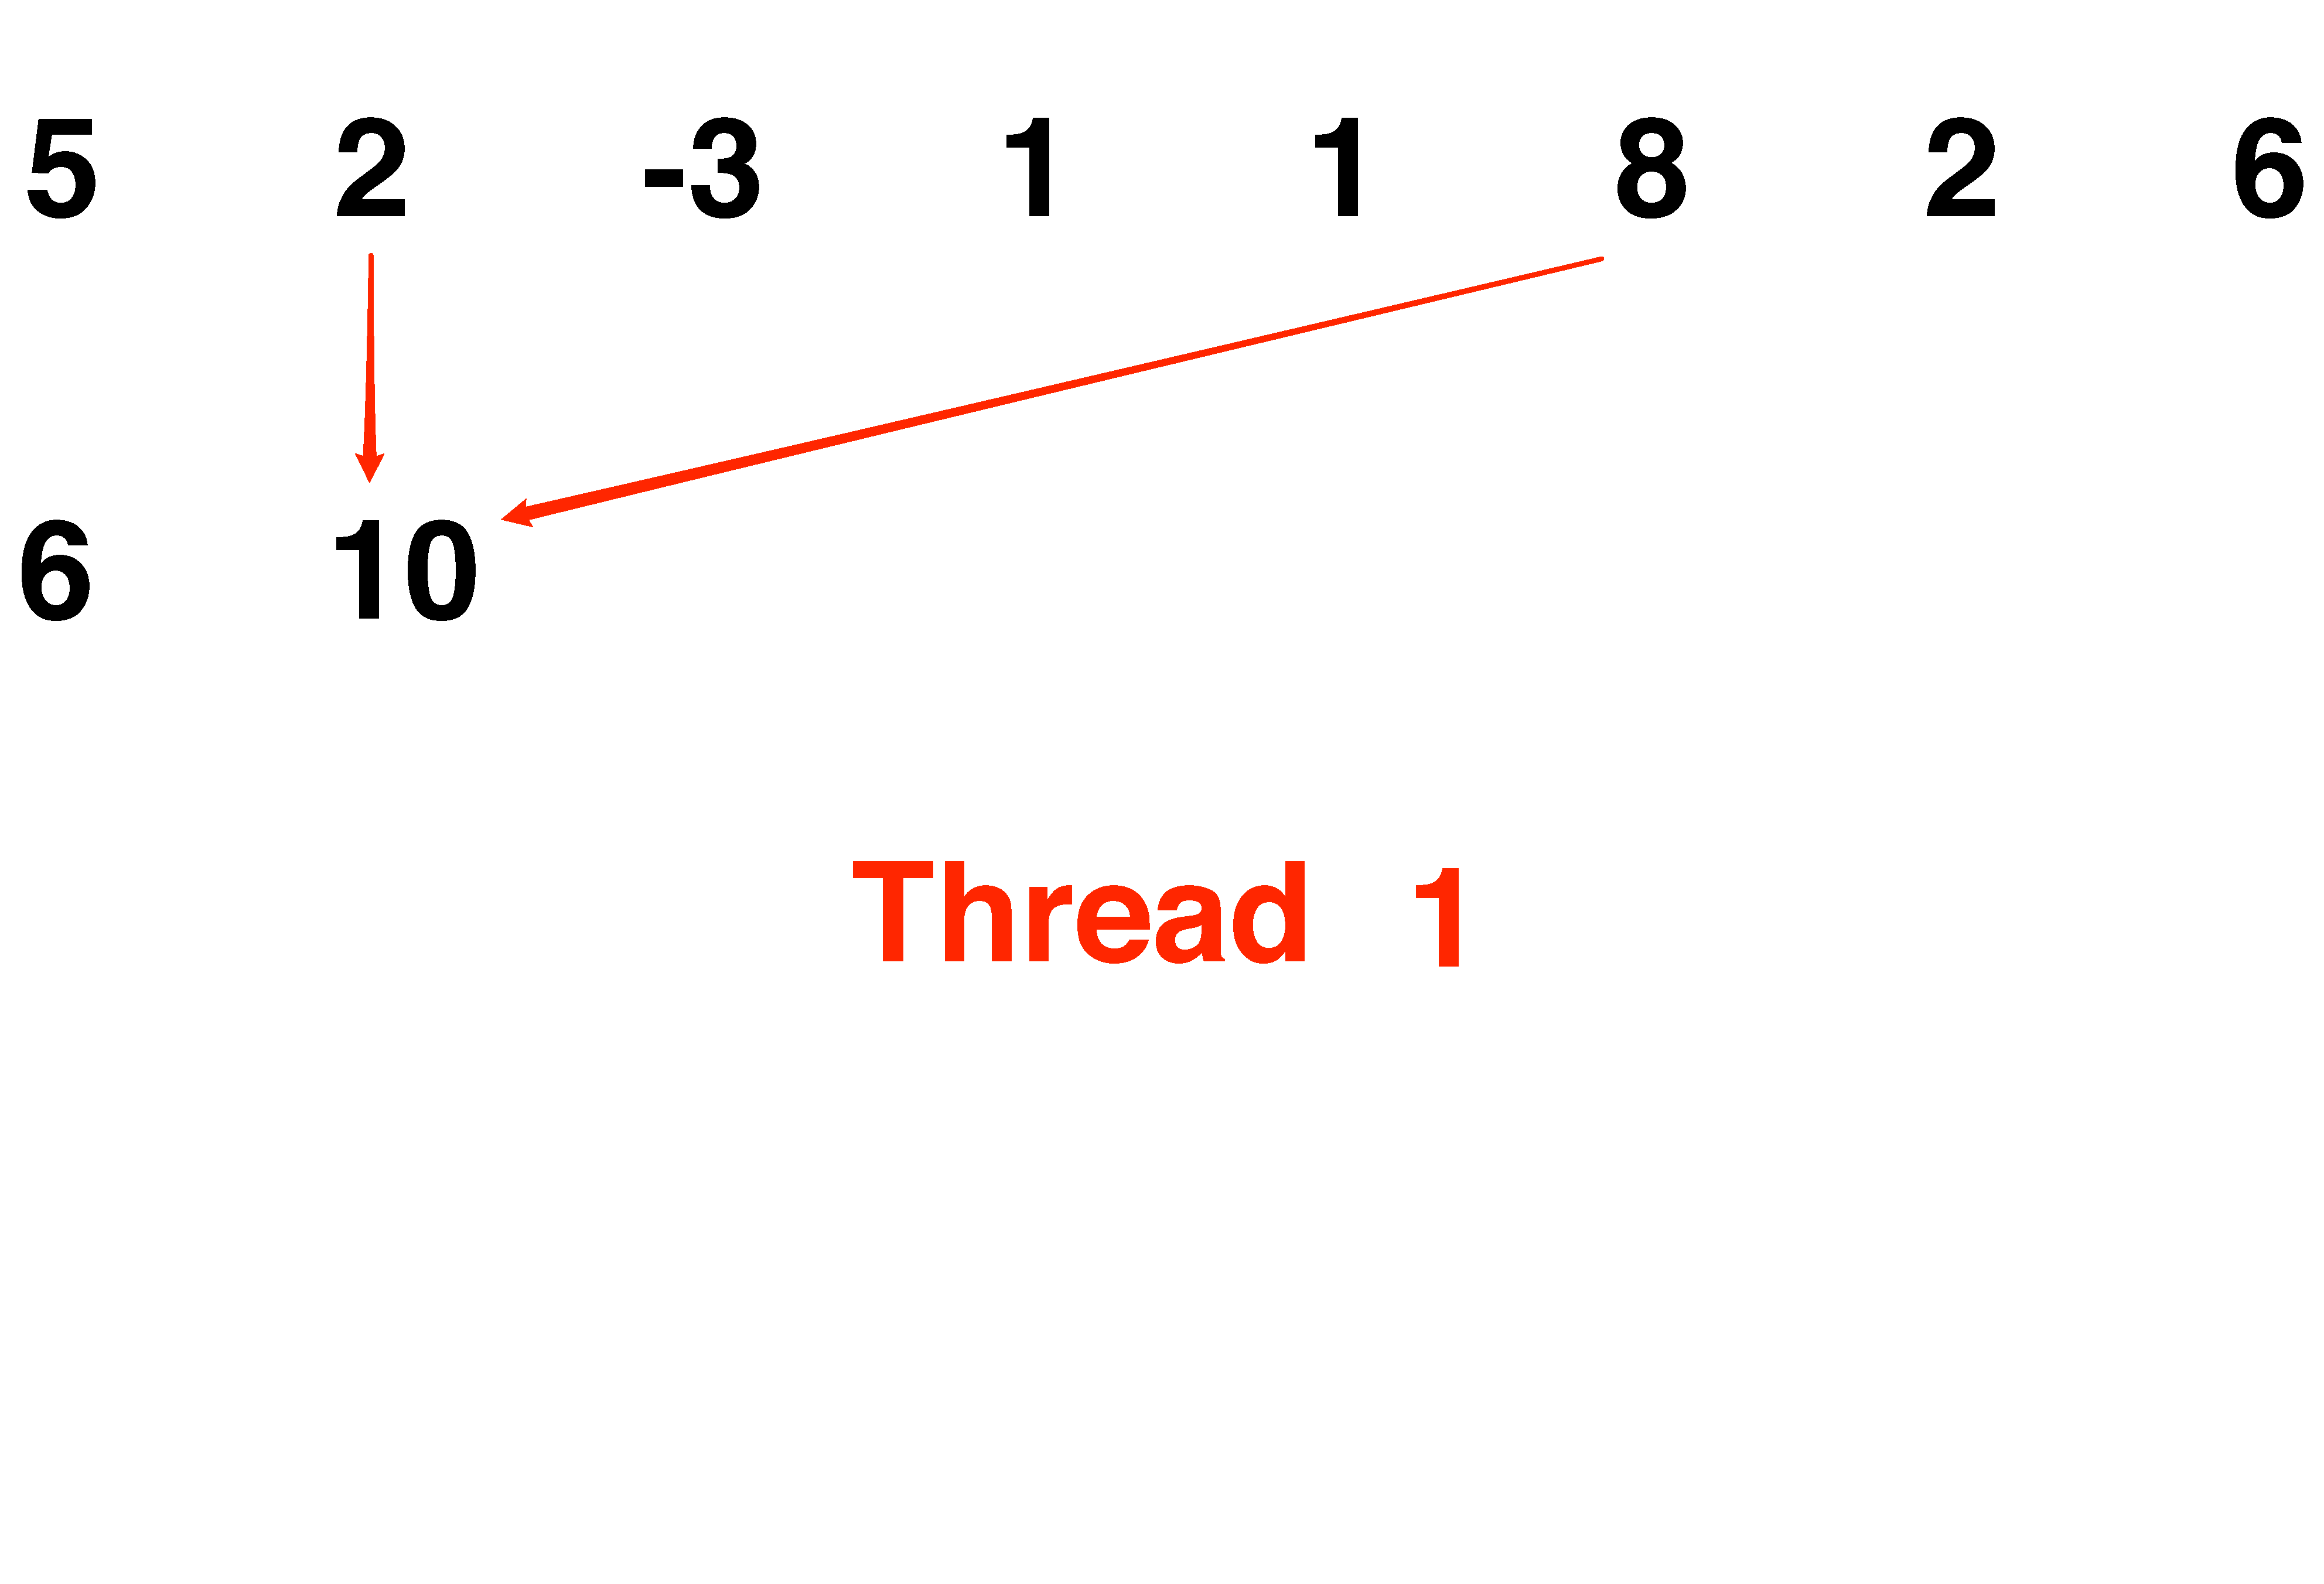
\includegraphics[scale=.15]{../../fig/psum2.pdf}
\end{frame}

\begin{frame}
\frametitle{Pairwise sum}
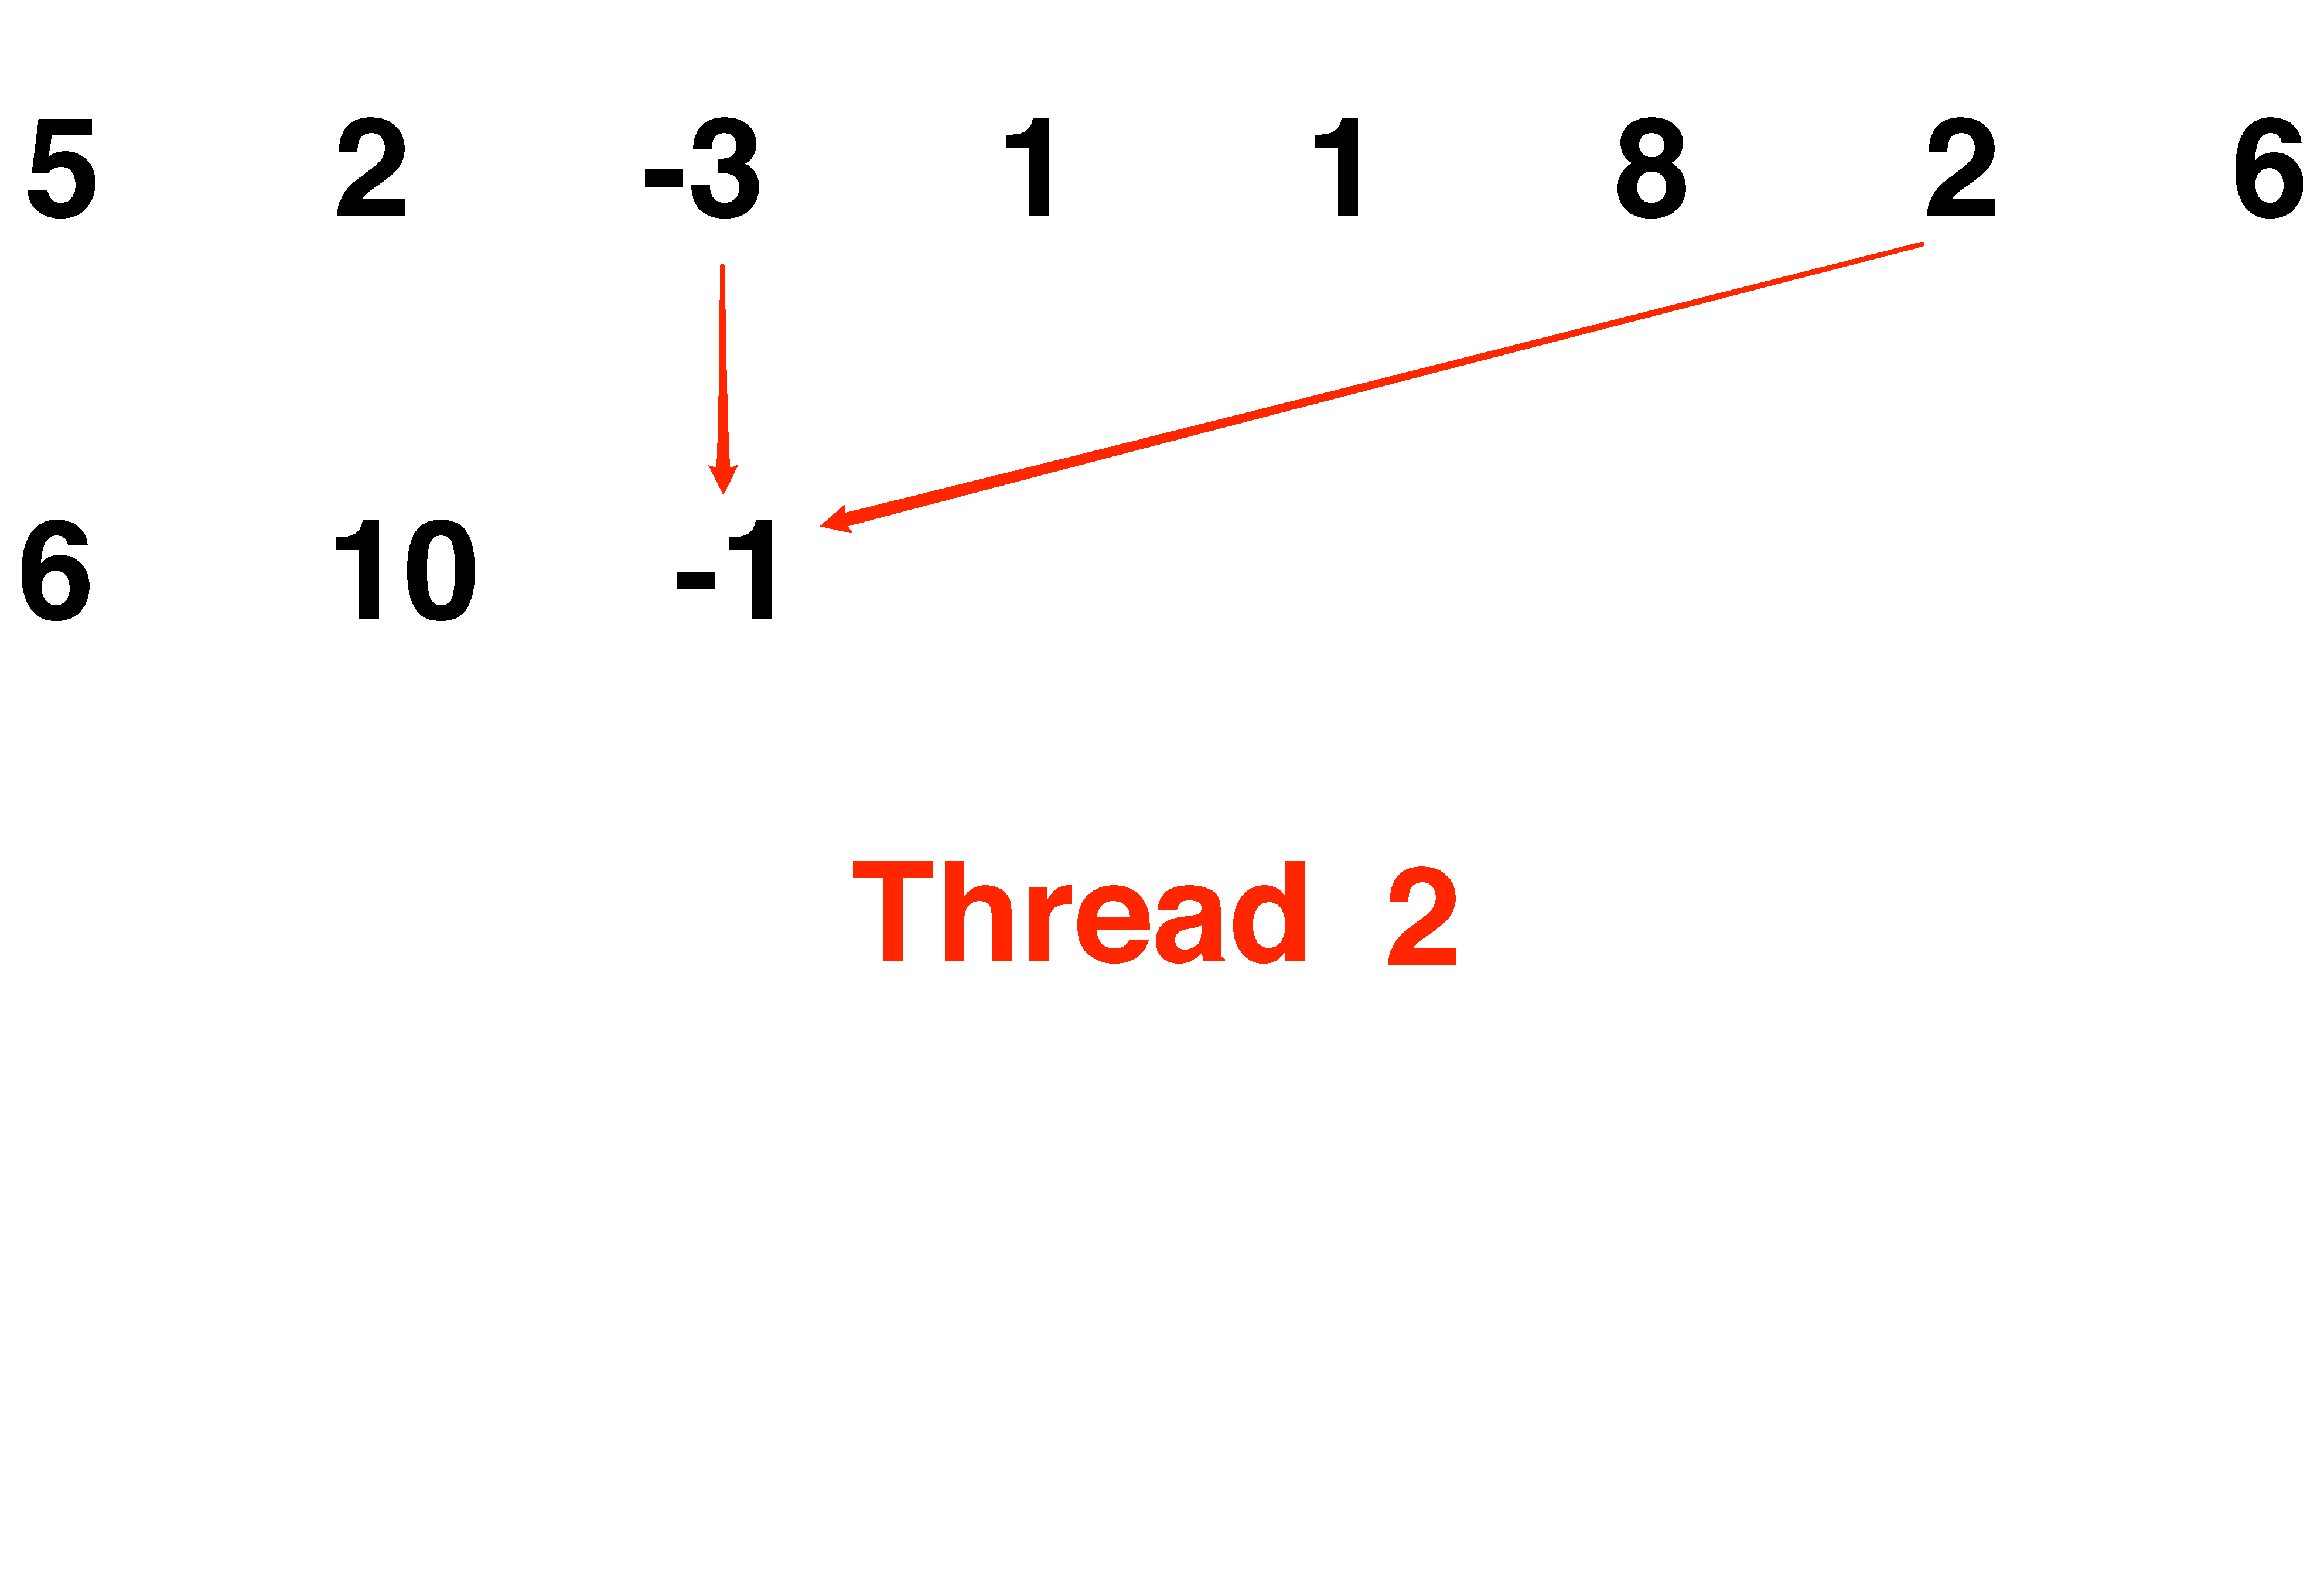
\includegraphics[scale=.15]{../../fig/psum3.pdf}
\end{frame}

\begin{frame}
\frametitle{Pairwise sum}
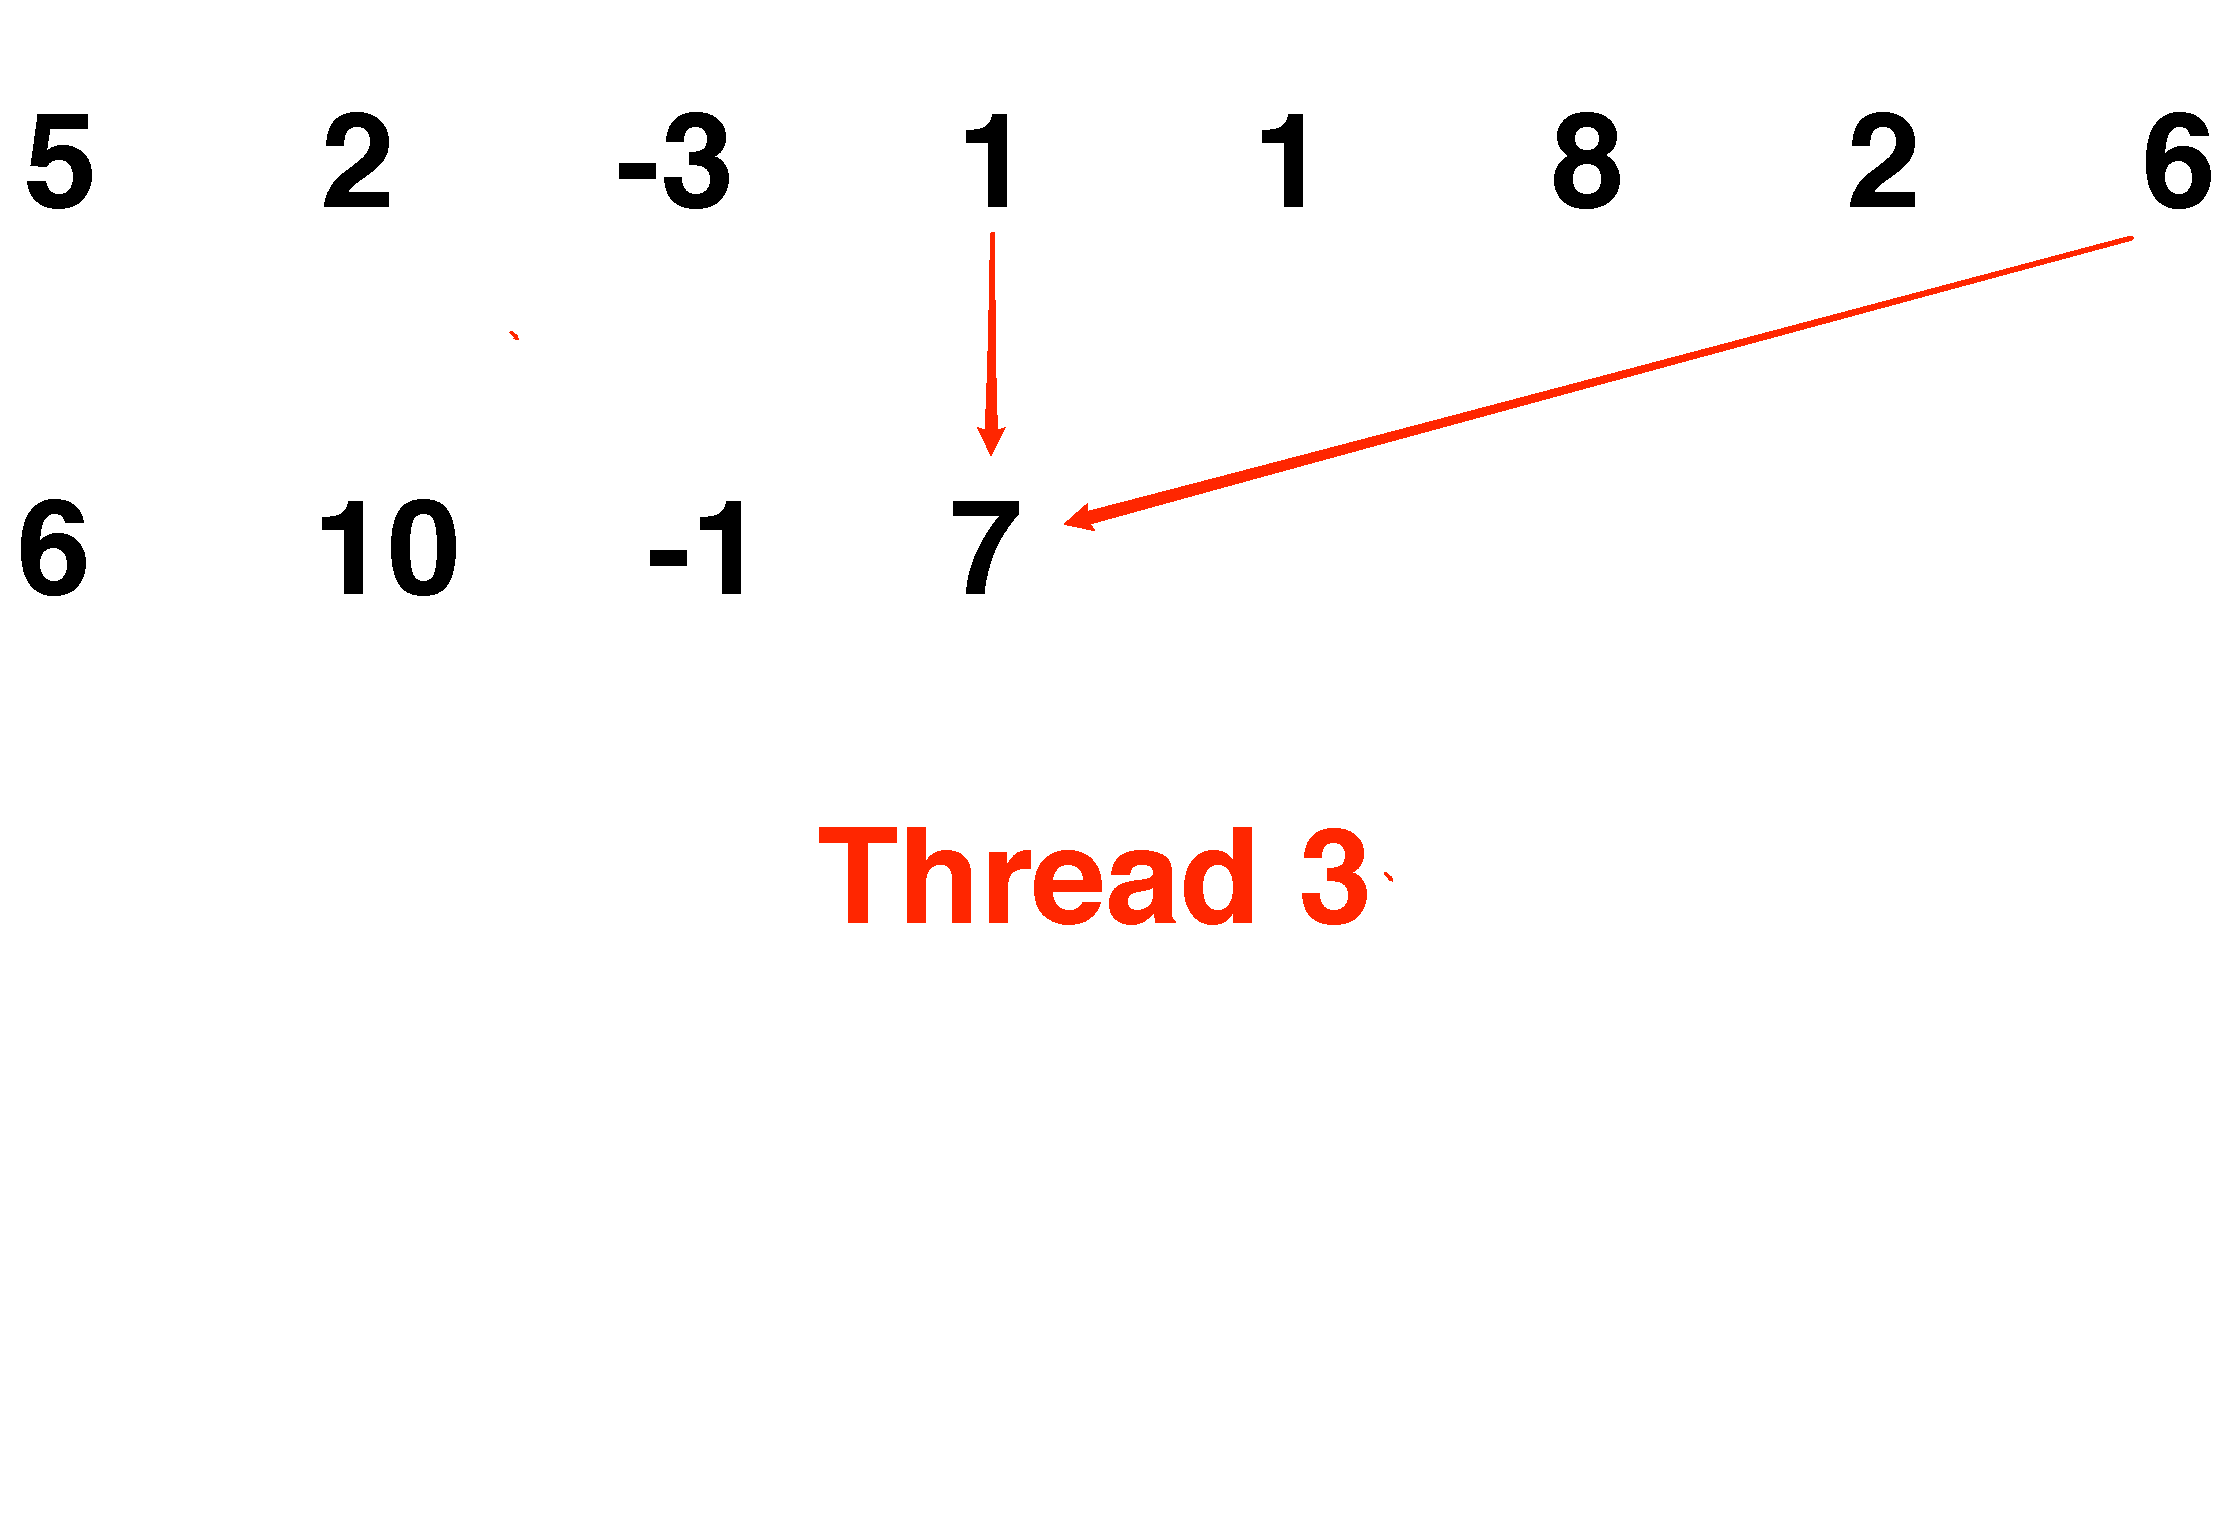
\includegraphics[scale=.25]{../../fig/psum4.pdf}
\end{frame}

\begin{frame}
\frametitle{Pairwise sum}
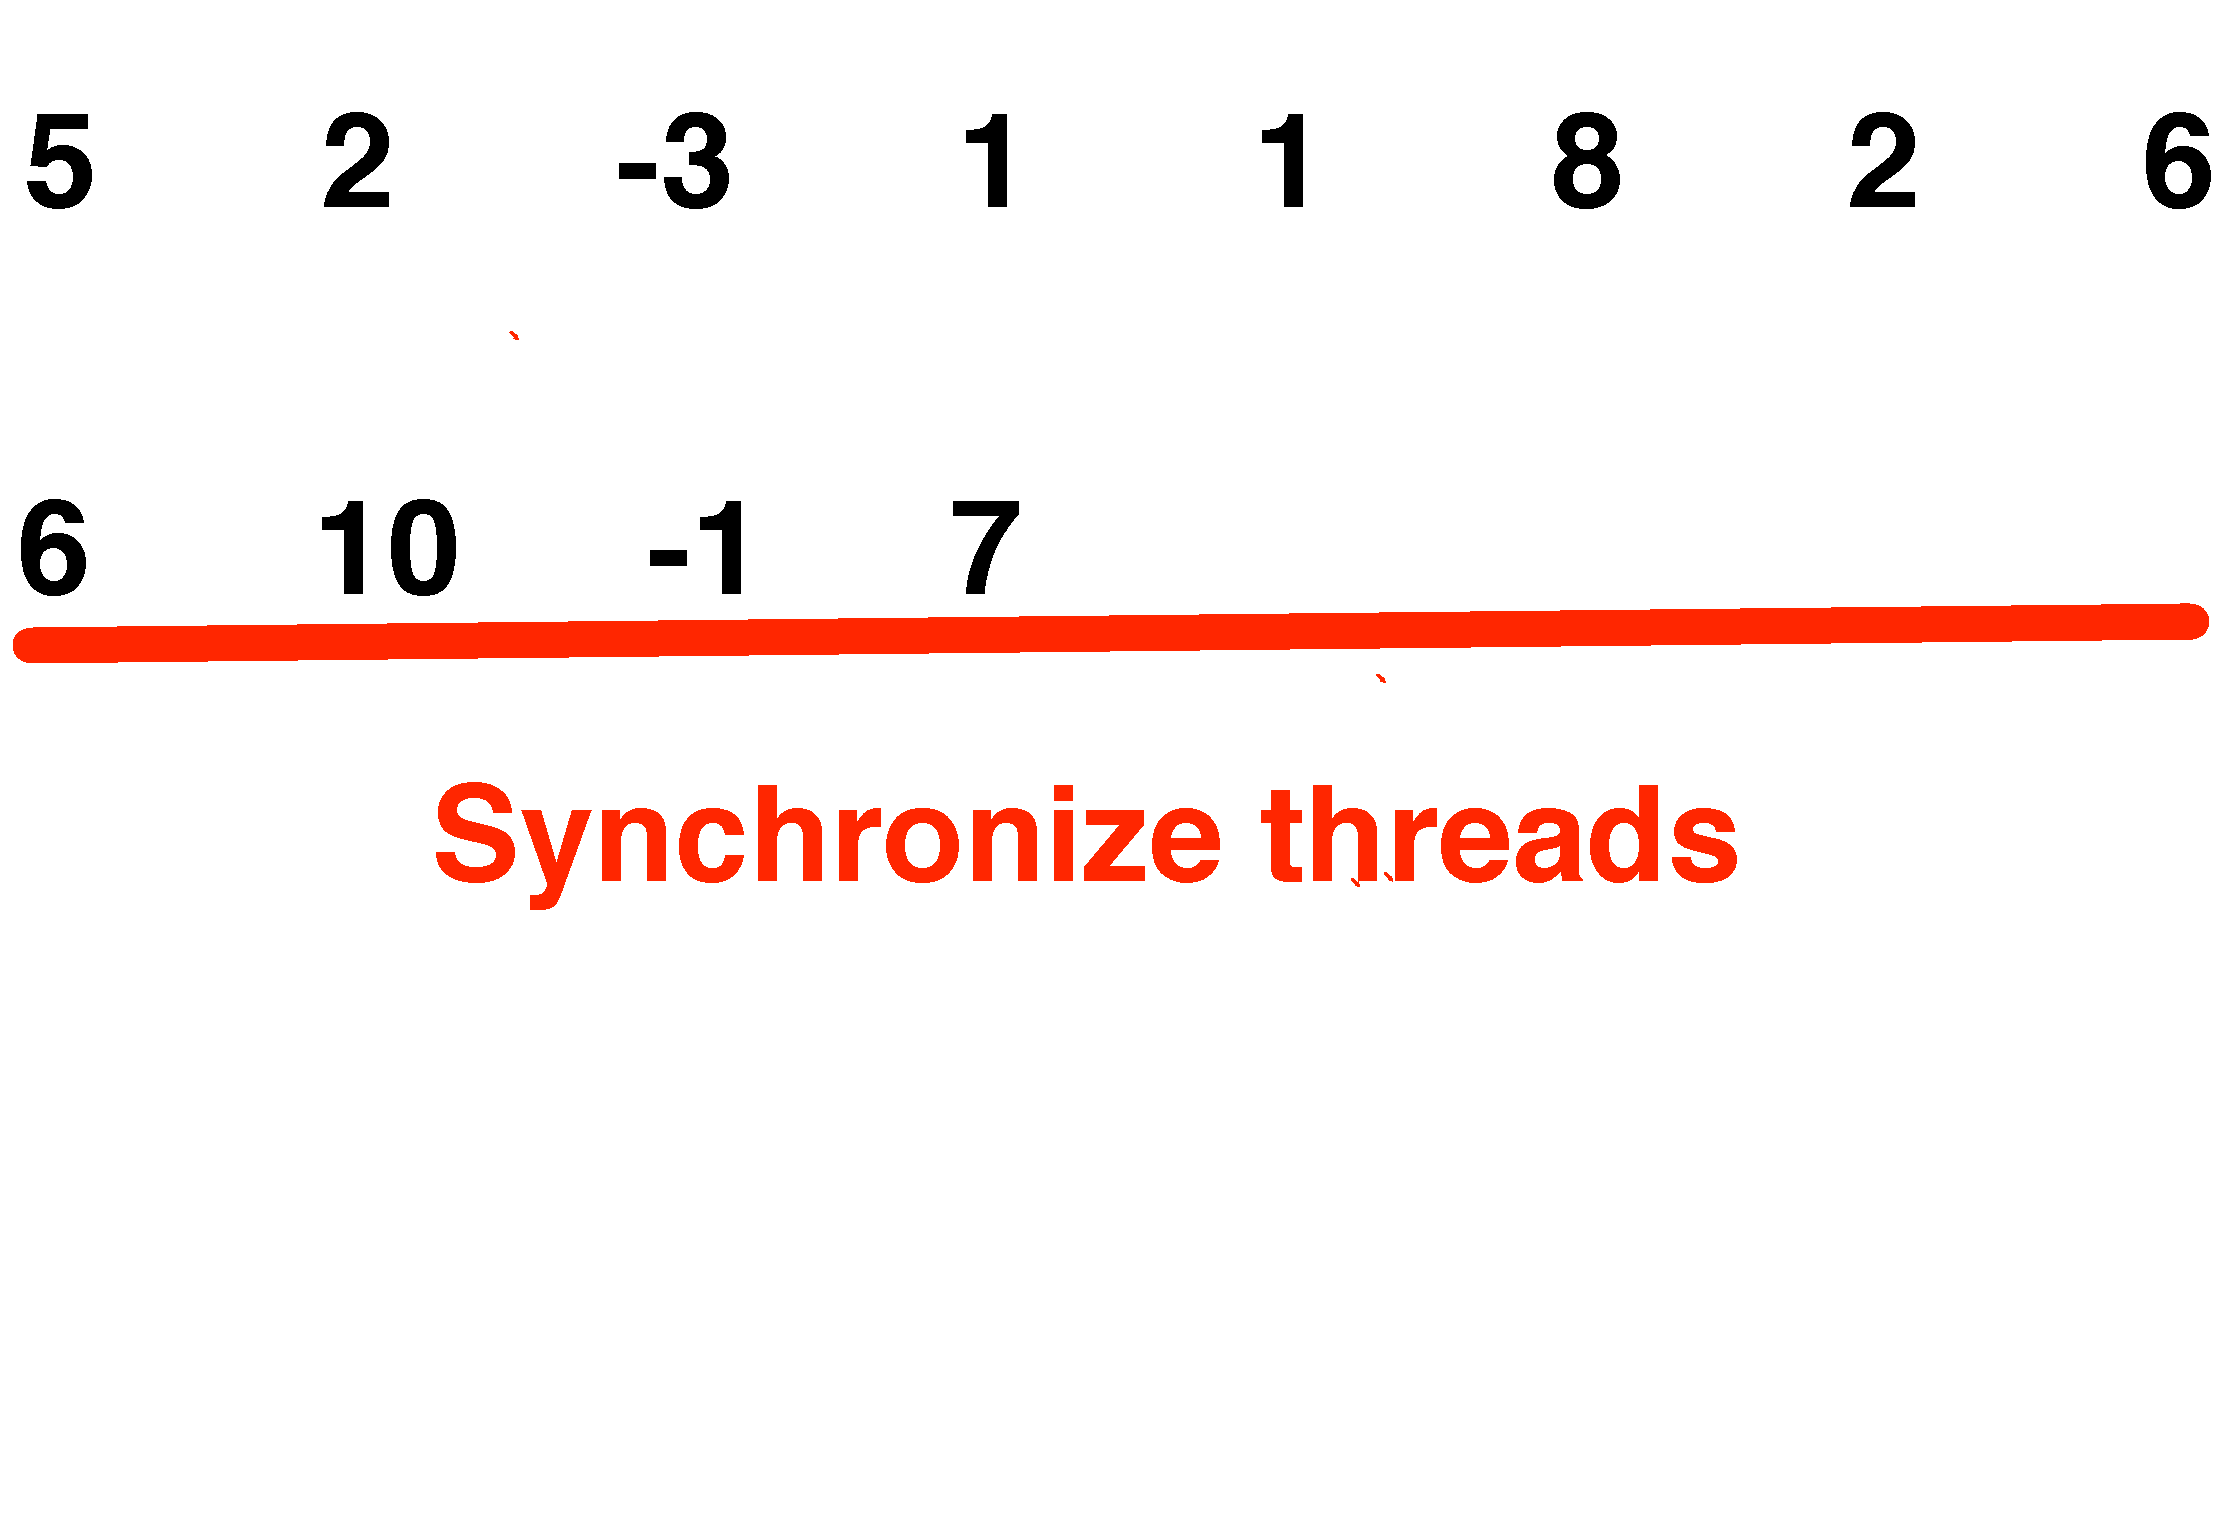
\includegraphics[scale=.25]{../../fig/psum5.pdf}
\end{frame}

\begin{frame}
\frametitle{Pairwise sum}
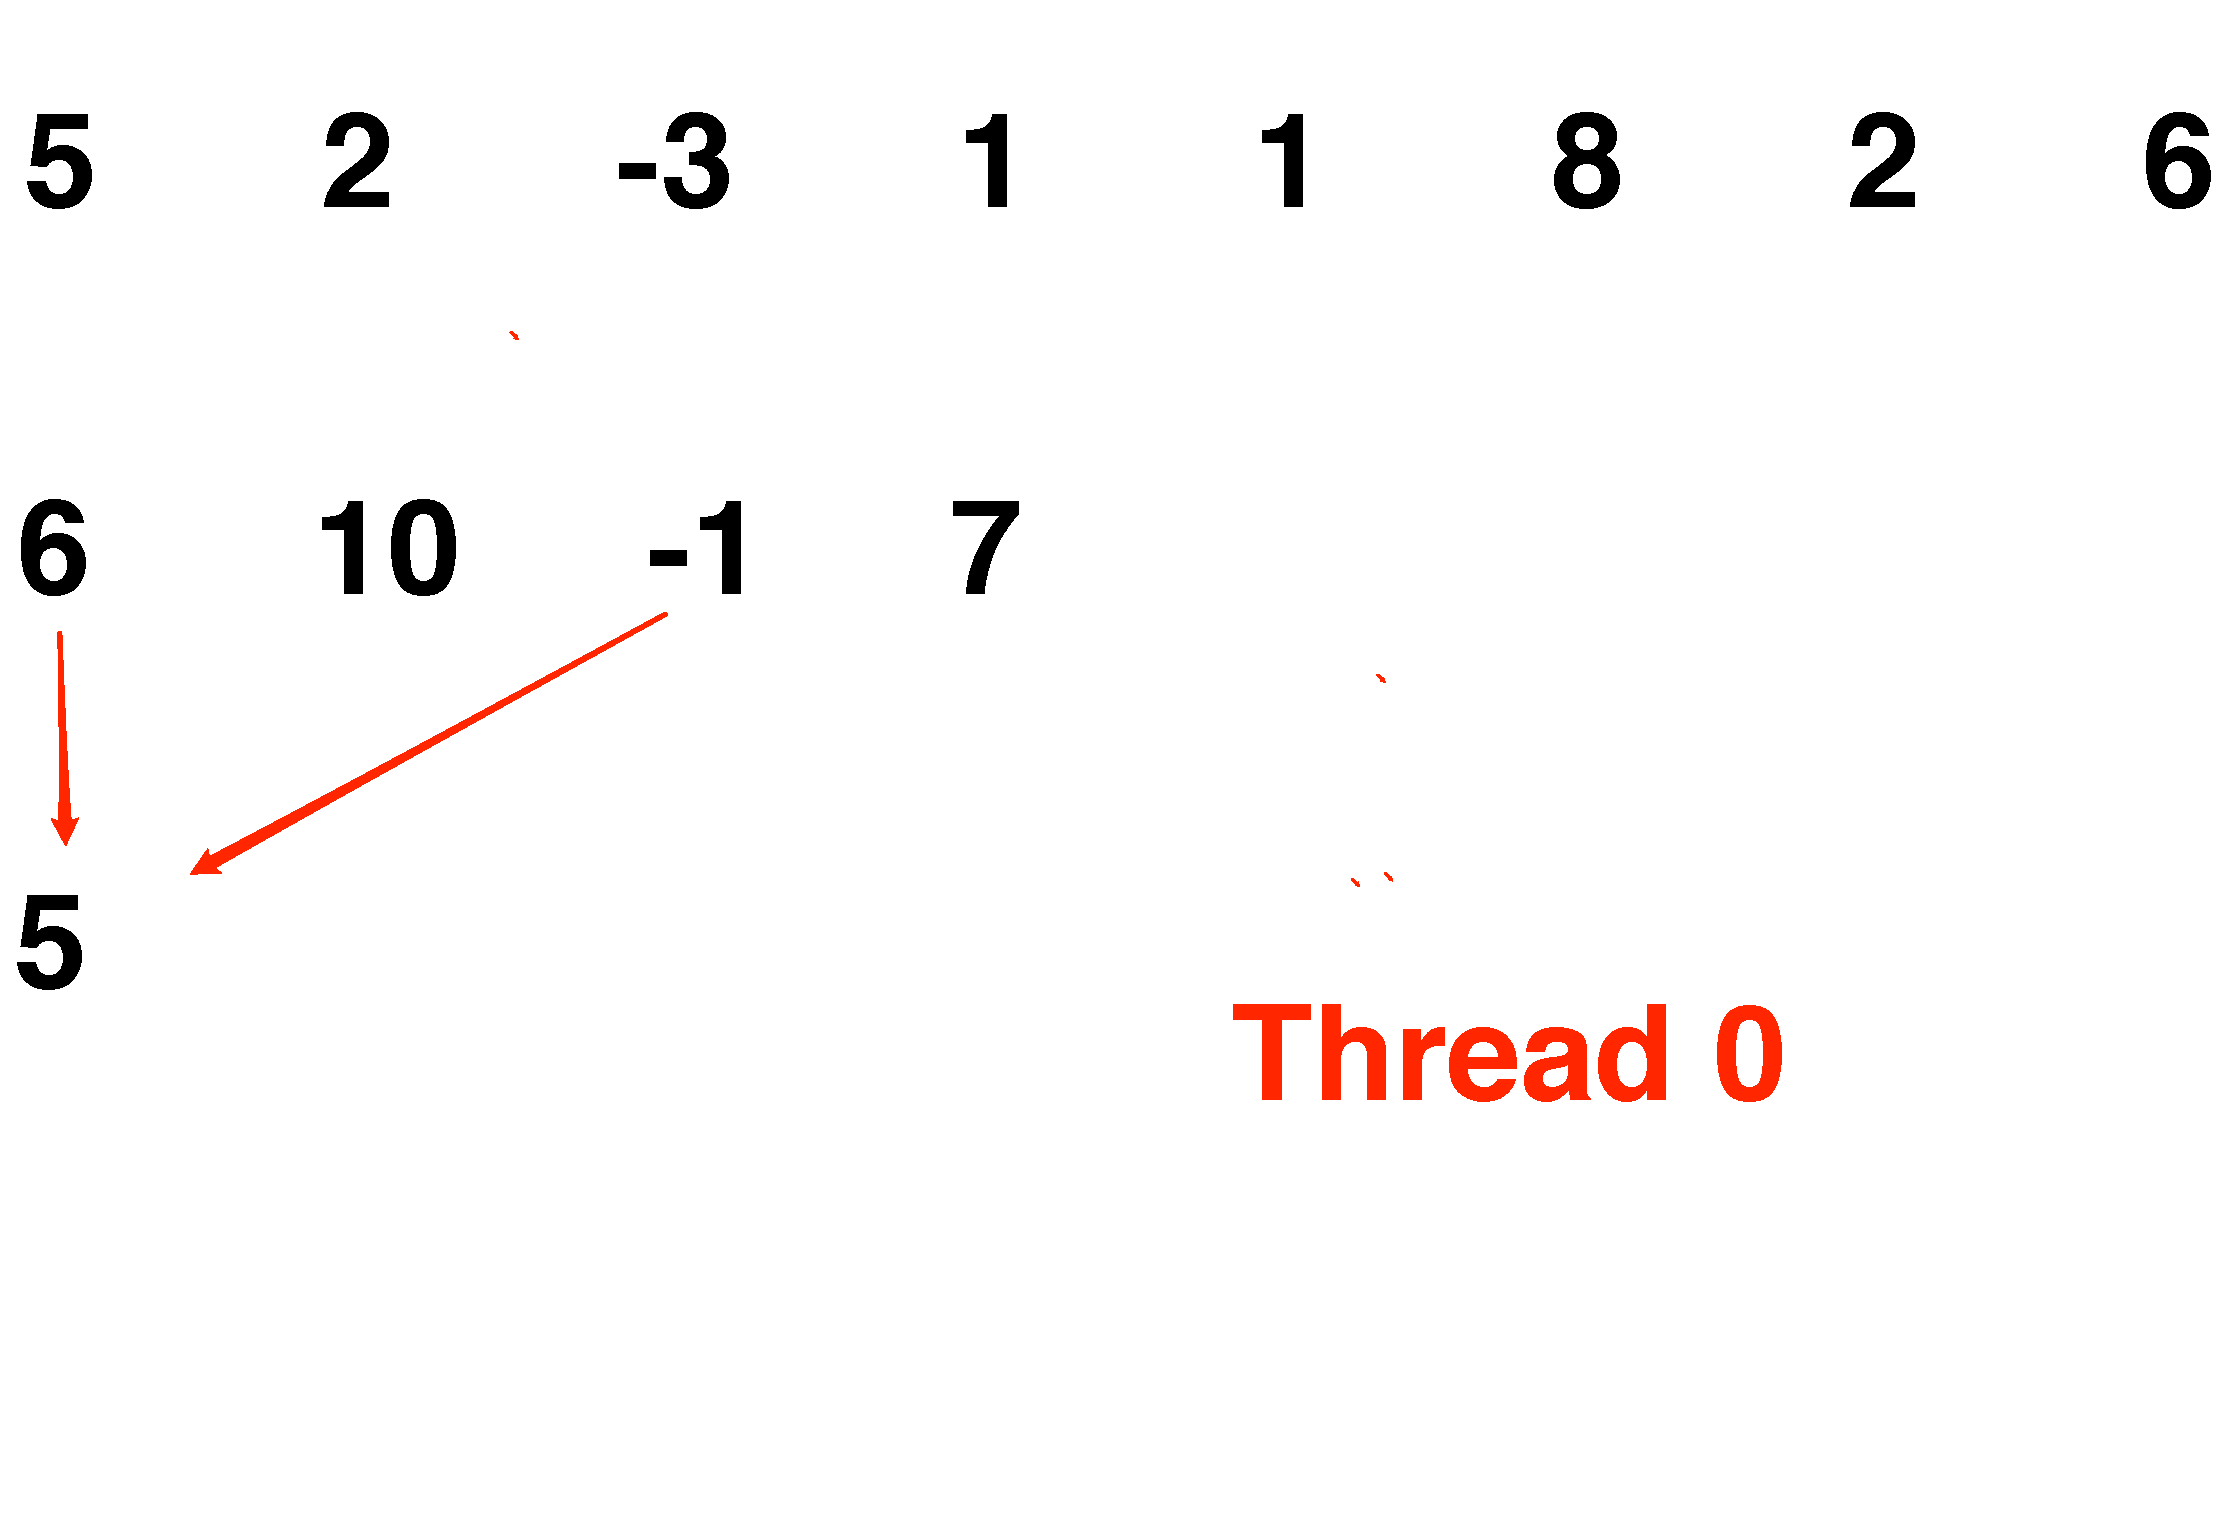
\includegraphics[scale=.25]{../../fig/psum6.pdf}
\end{frame}

\begin{frame}
\frametitle{Pairwise sum}
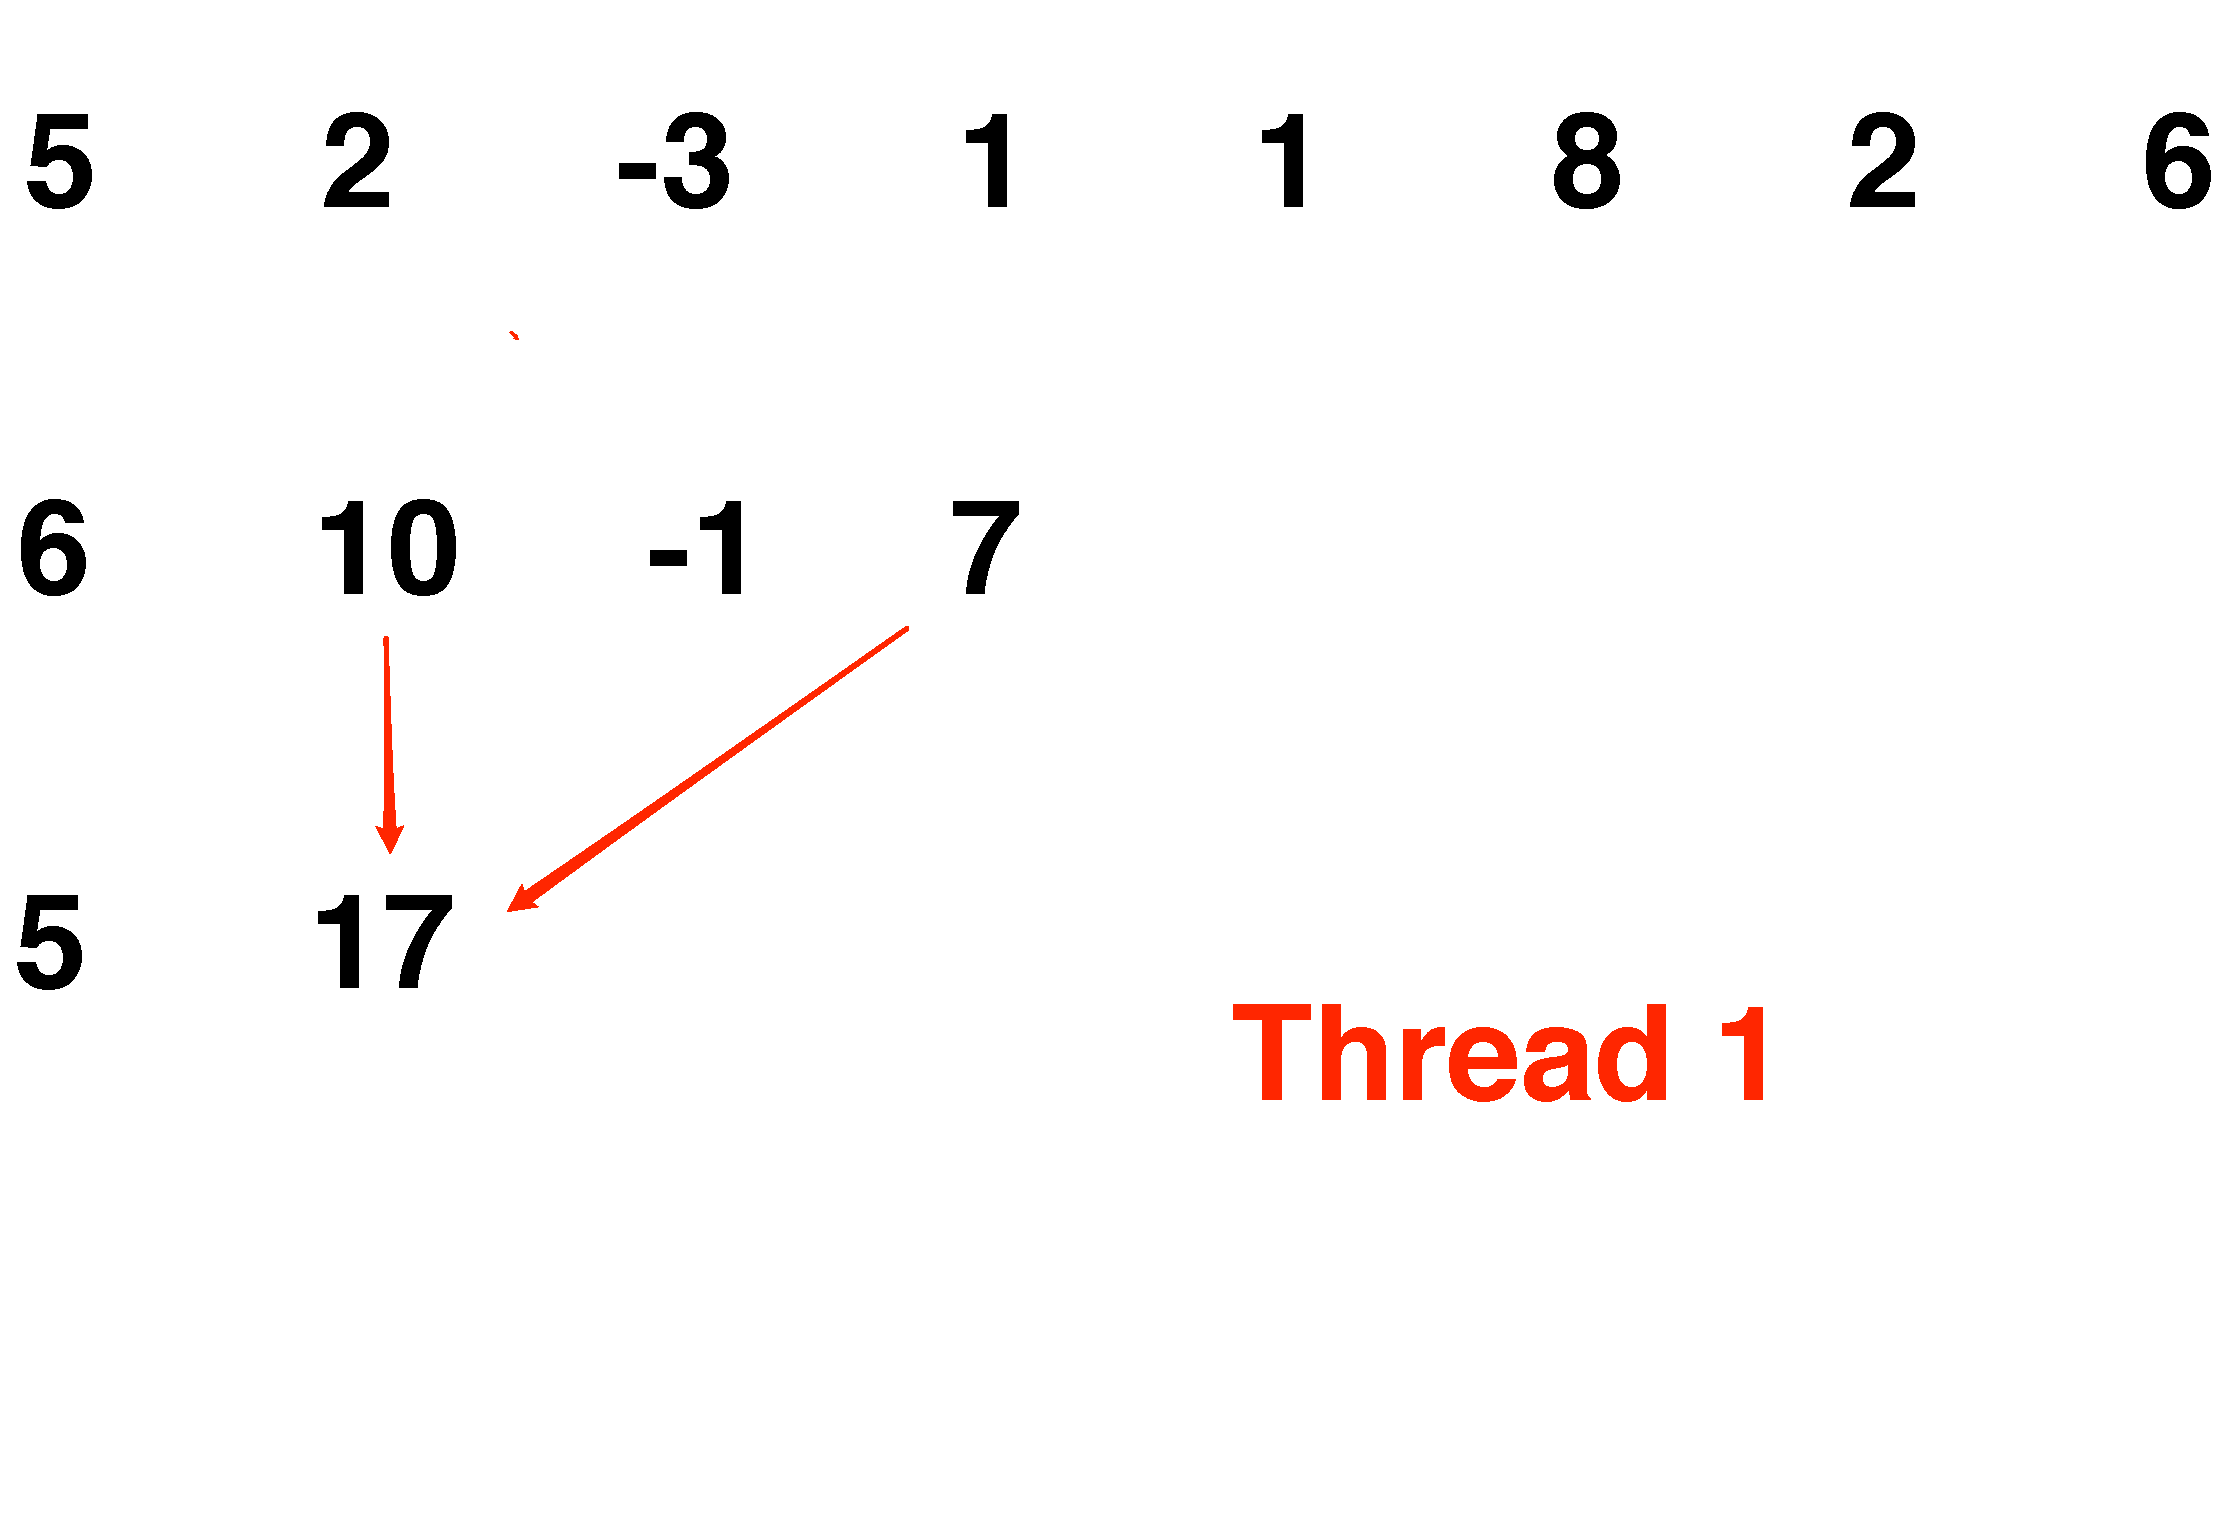
\includegraphics[scale=.25]{../../fig/psum7.pdf}
\end{frame}

\begin{frame}
\frametitle{Pairwise sum}
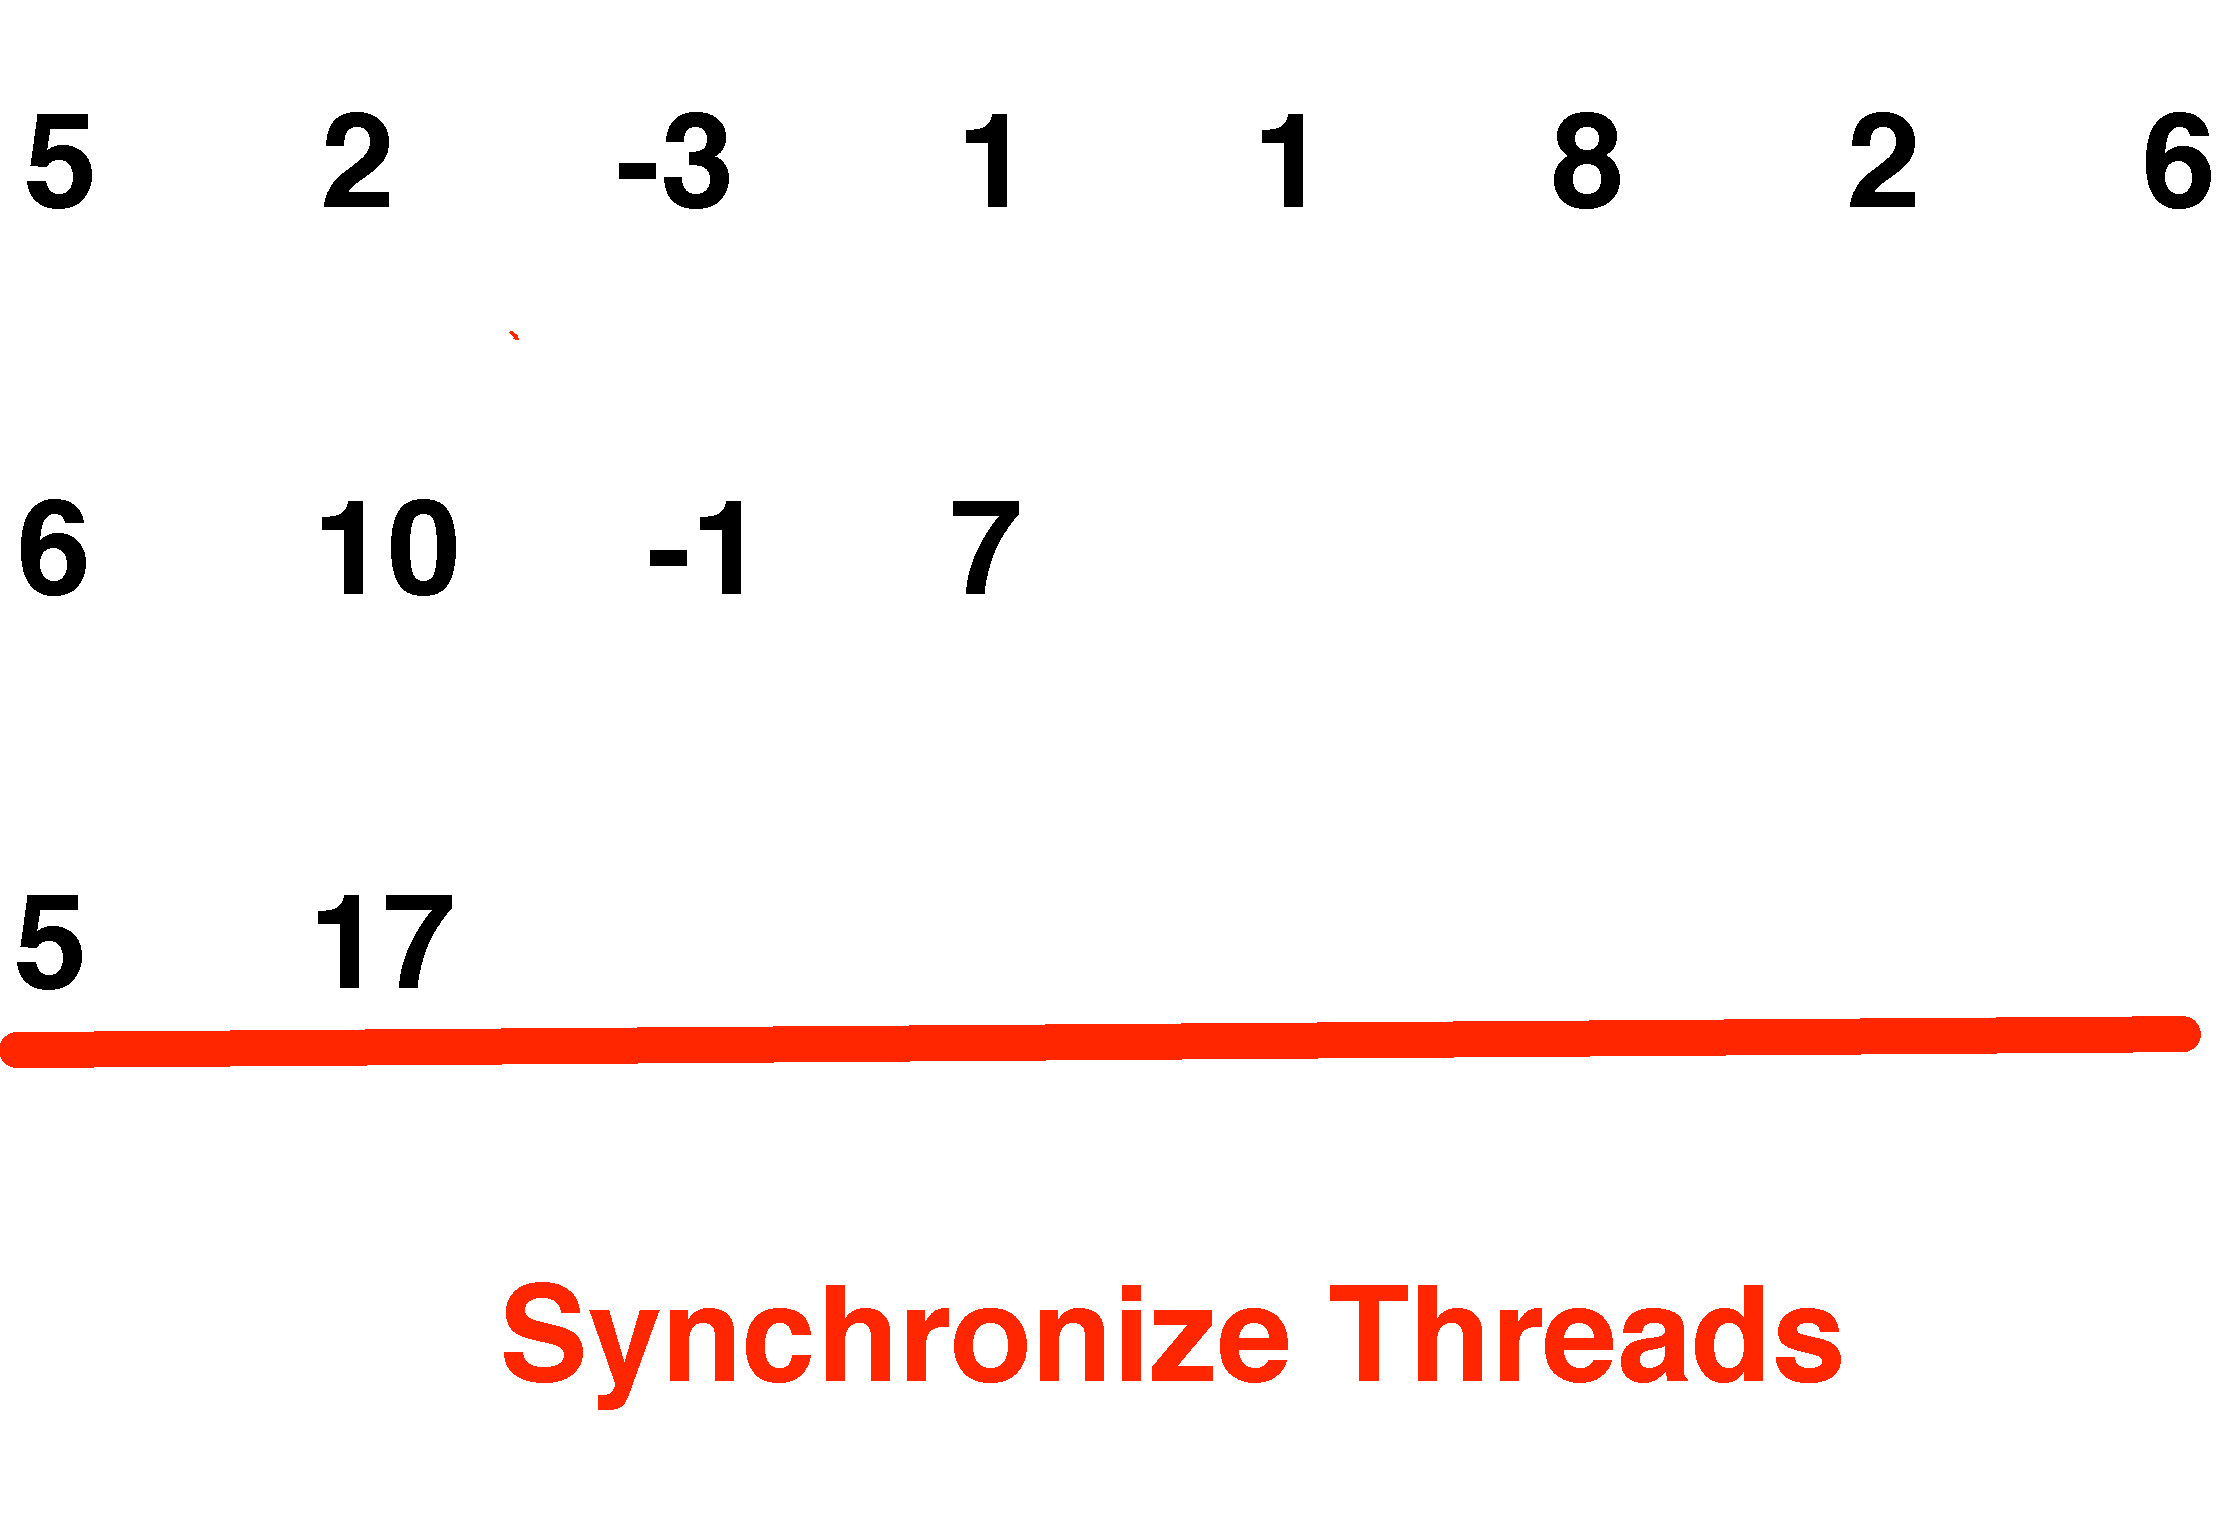
\includegraphics[scale=.25]{../../fig/psum8.pdf}
\end{frame}

\begin{frame}
\frametitle{Pairwise sum}
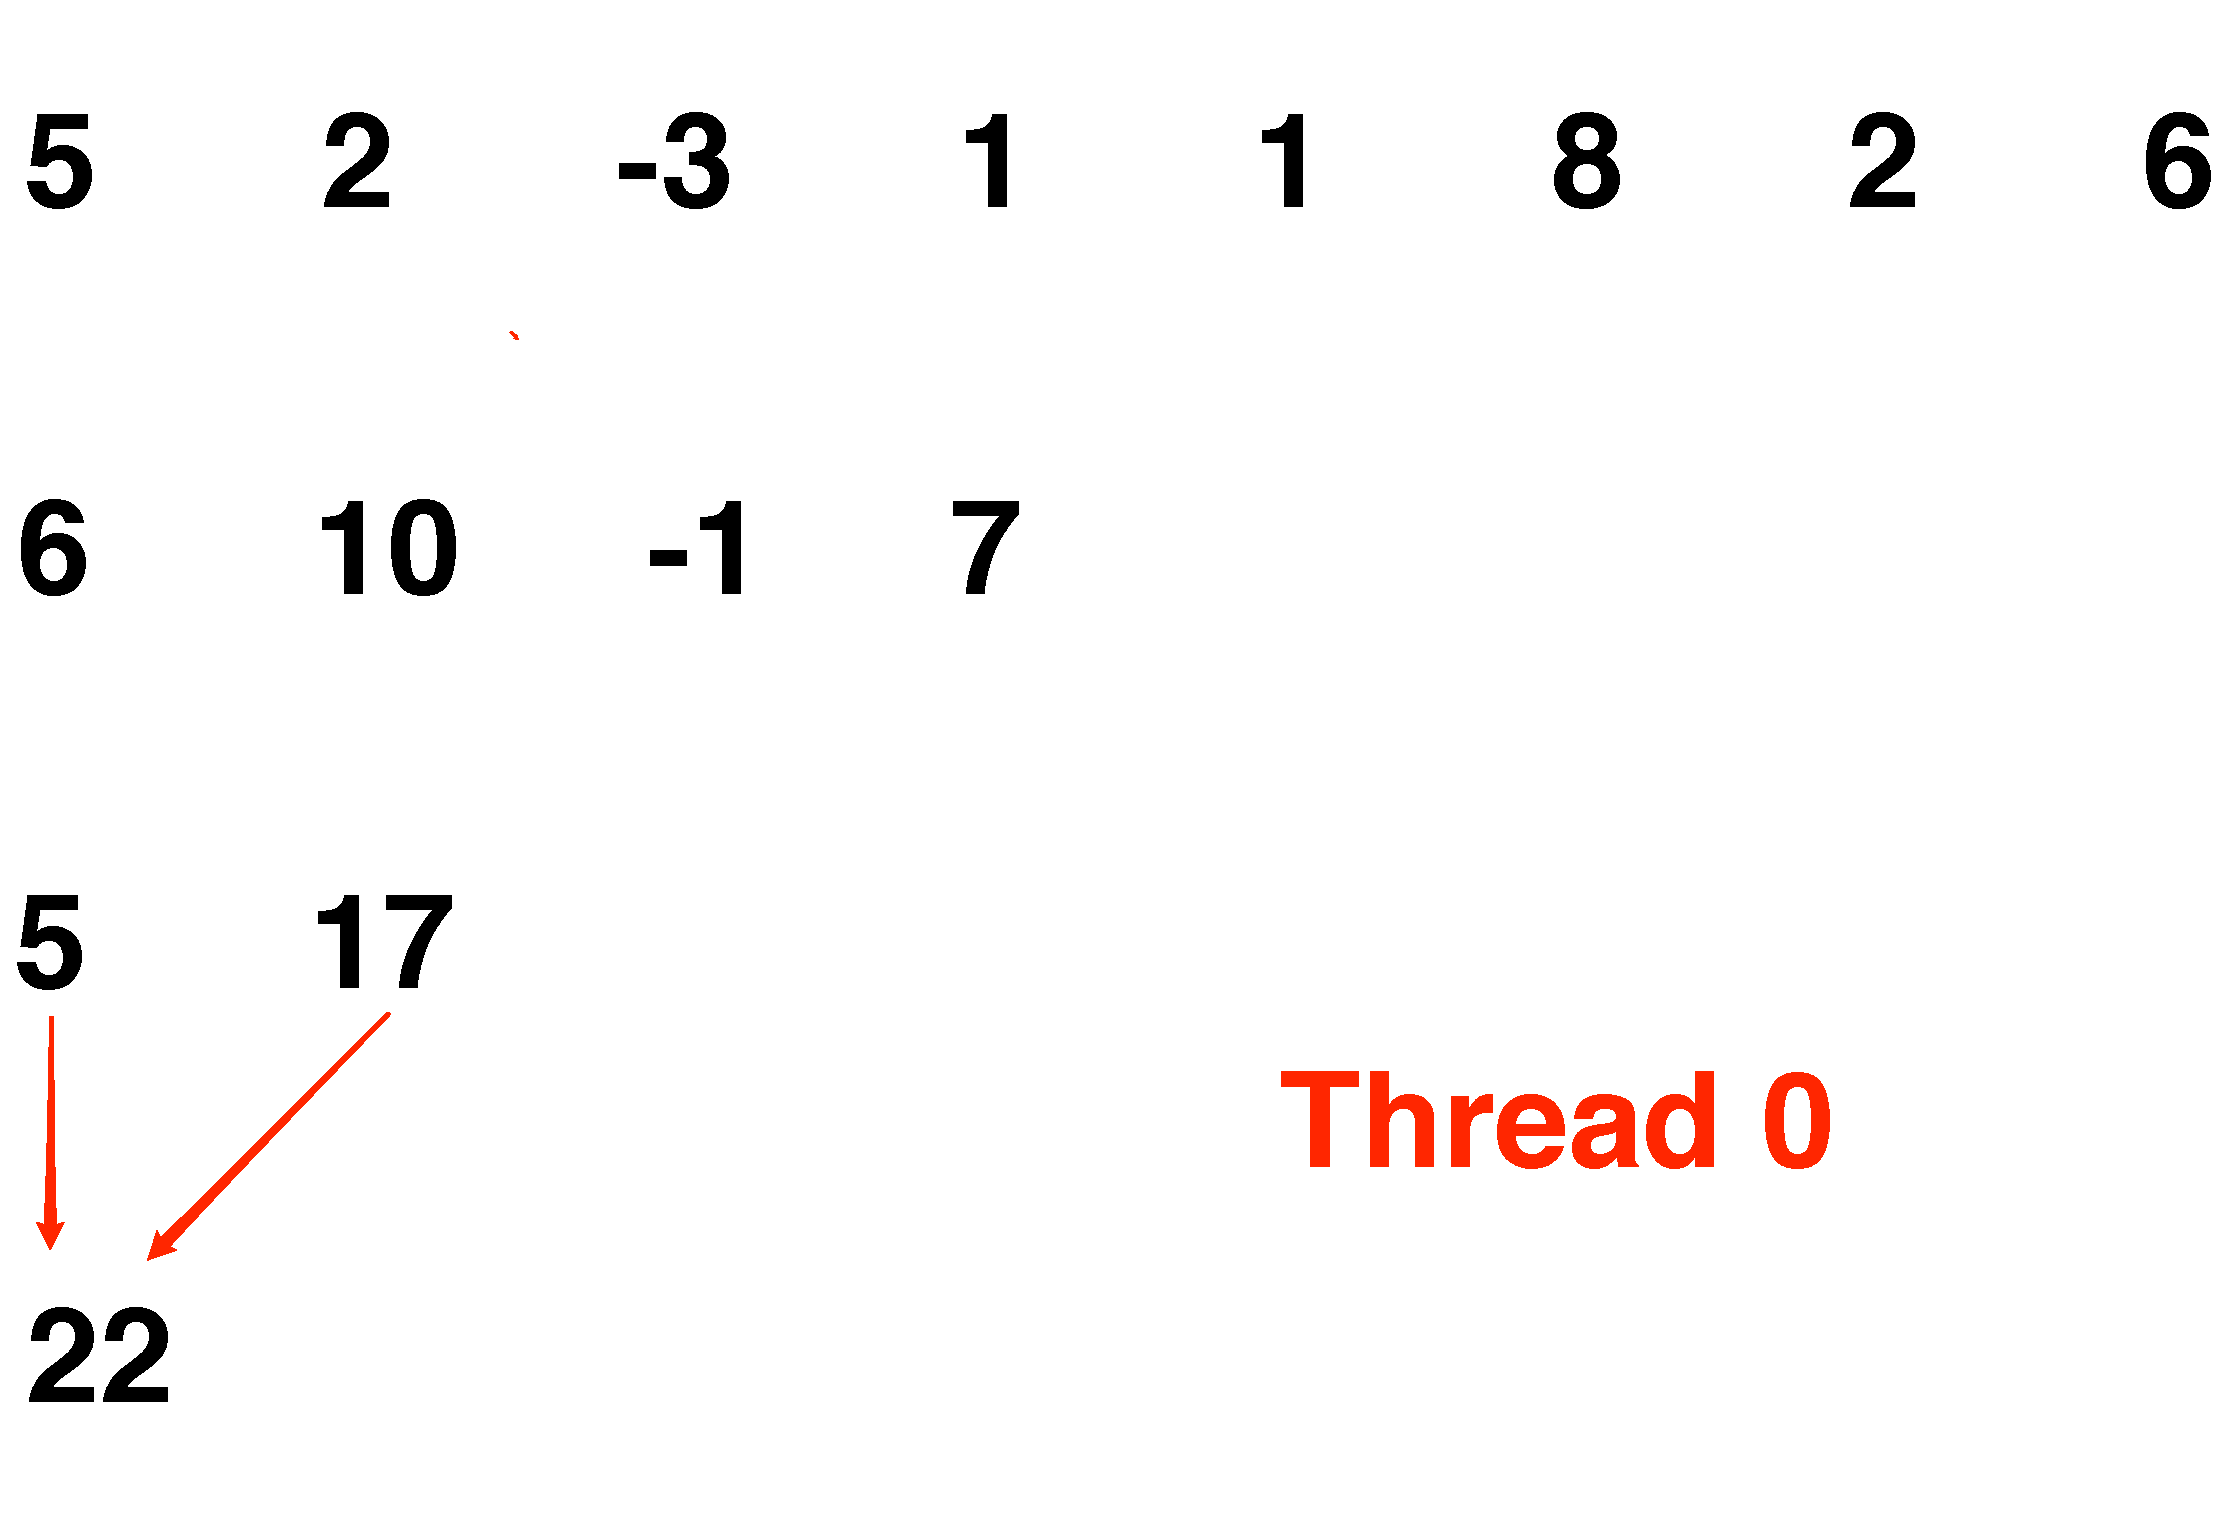
\includegraphics[scale=.25]{../../fig/psum9.pdf}
\end{frame}

\begin{frame}
\frametitle{Synchronizing threads}
\begin{itemize}
\item {\bf Synchronization}: waiting for all parallel tasks to reach a checkpoint before allowing any of then to continue.
\begin{itemize}
\pause \item Threads from the same block can be synchronized easily.
\pause \item In general, do not try to synchronize threads from different blocks. It's possible, but extremely inefficient.
\end{itemize}
\end{itemize}
\end{frame}


\begin{frame}
\frametitle{Compare the pairwise sum to the sequential sum}
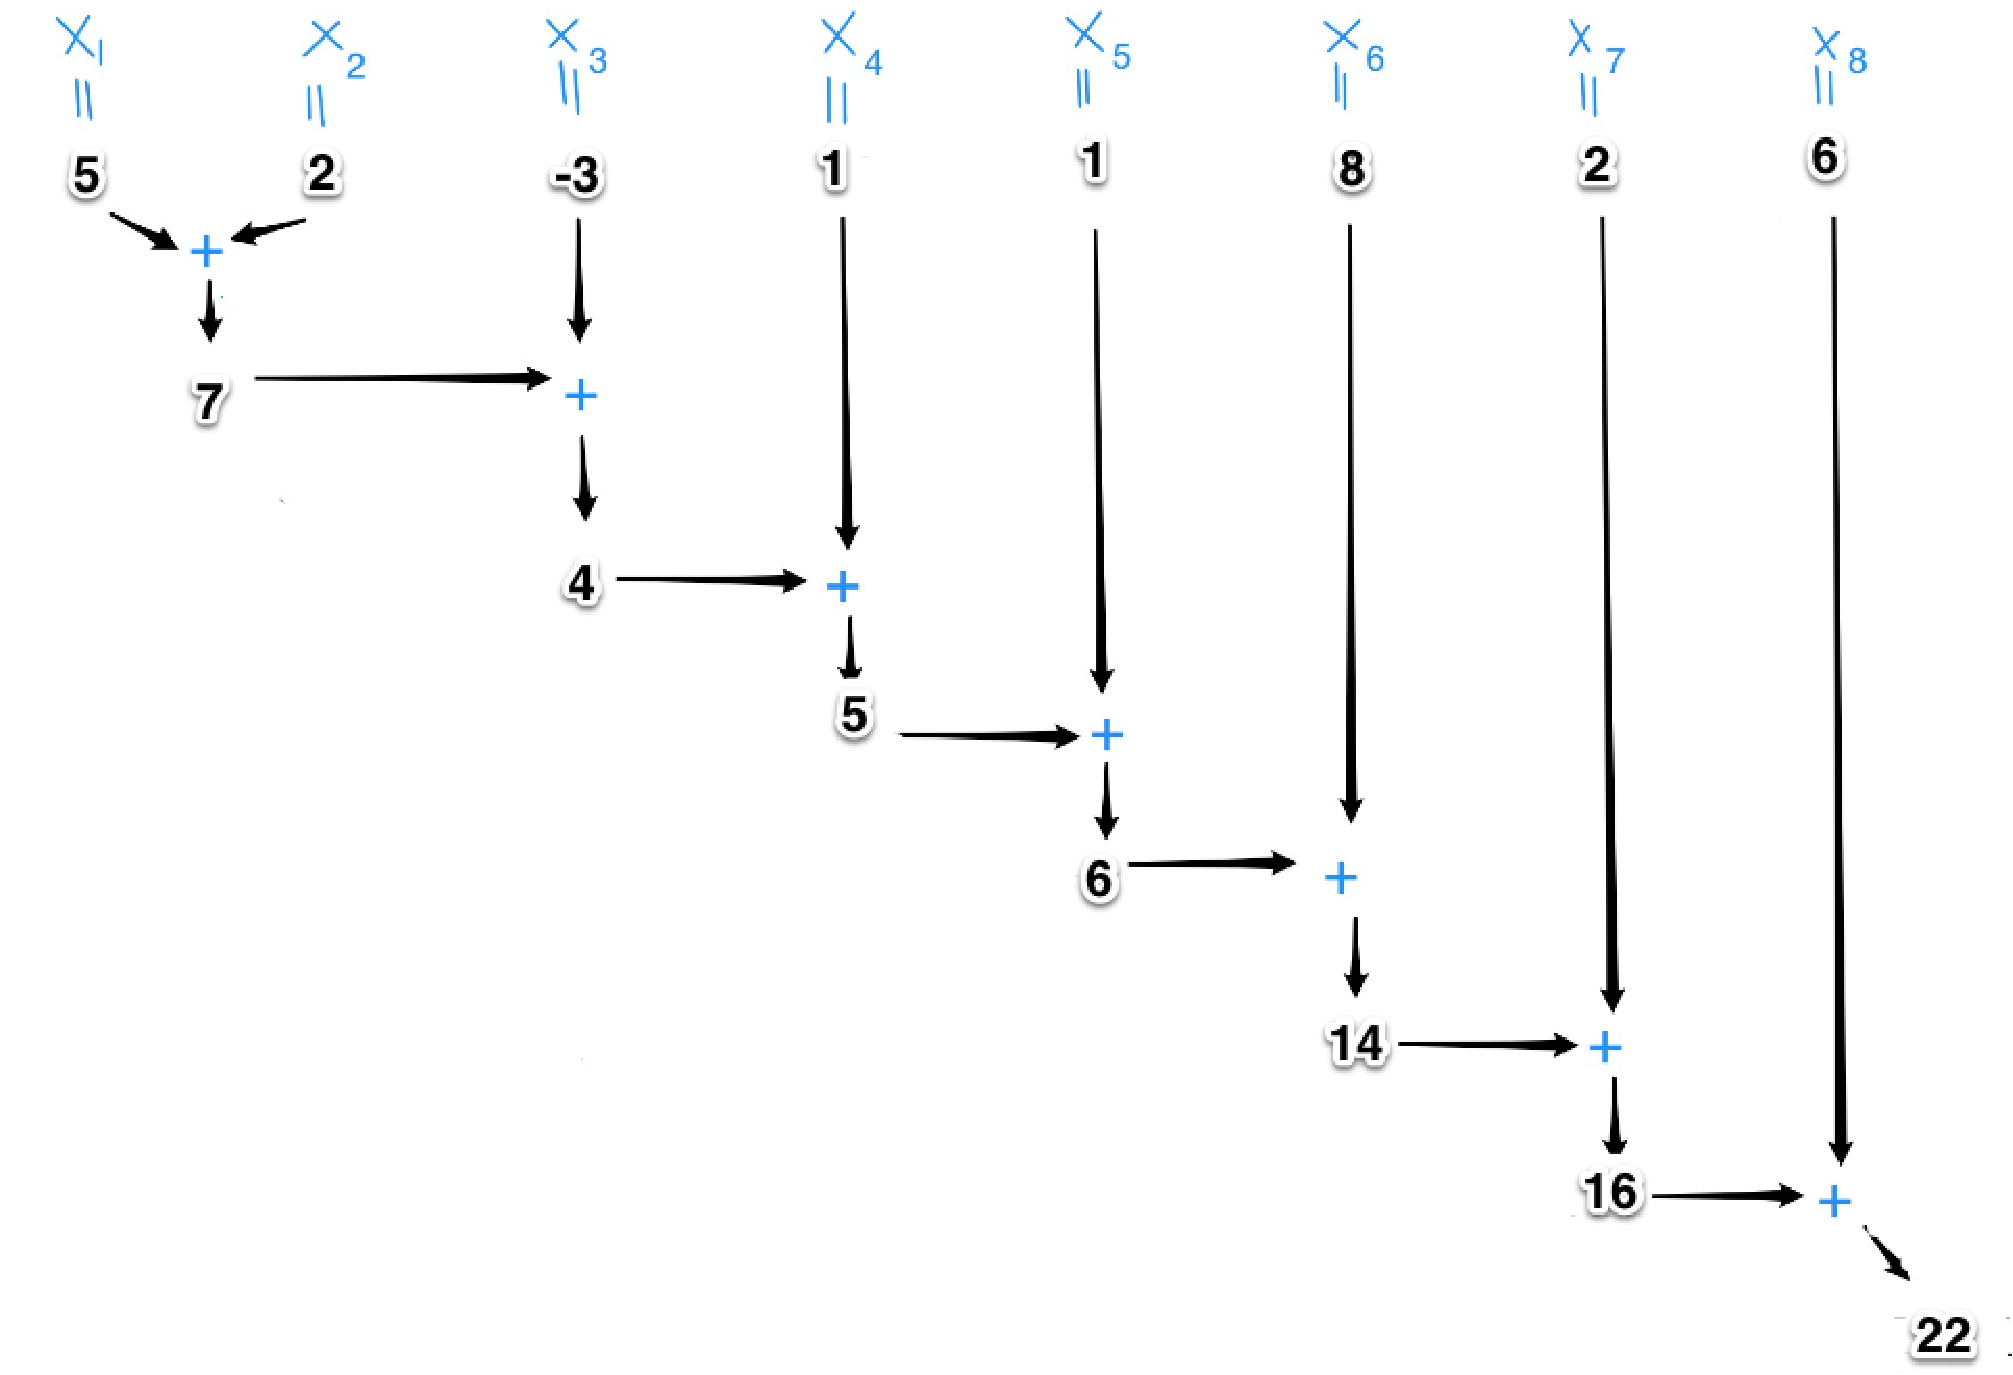
\includegraphics[scale=.25]{../../fig/sequential}
\begin{itemize}
\item The pairwise sum requires only $\log_2(n)$ sequential stages, while the sequential sum requires $n-1$ sequential steps.
\end{itemize}
\end{frame}

\begin{frame}[fragile]
\frametitle{{\tt pairwise\_sum.cu}}\lstset{basicstyle=\tiny}
\begin{lstlisting}[name=ps]
#include <stdio.h> 
#include <stdlib.h> 
#include <math.h>
#include <cuda.h>
#include <cuda_runtime.h> 

/*
 * This program computes the sum of the elements of 
 * vector v using the pairwise (cascading) sum algorithm.
 */

#define N 8 // length of vector v. MUST BE A POWER OF 2!!!

// Fill the vector v with n random floating point numbers.
void vfill(float* v, int n){
  int i;
  for(i = 0; i < n; i++){
    v[i] = (float) rand() / RAND_MAX;
  }
}

// Print the vector v.
void vprint(float* v, int n){
  int i;
  printf("v = \n");
  for(i = 0; i < n; i++){
    printf("%7.3f\n", v[i]);
  }
  printf("\n");
}
\end{lstlisting}
\end{frame}


\begin{frame}[fragile]
\frametitle{{\tt pairwise\_sum.cu}} \lstset{basicstyle=\tiny}
\begin{lstlisting}[name=ps]
// Pairwise-sum the elements of vector v and store the result in v[0]. 
__global__ void psum(float* v){ 
  int t = threadIdx.x; // Thread index.
  int n = blockDim.x; // Should be half the length of v.

  while (n != 0) {
    if(t < n)
      v[t] += v[t + n];  
    __syncthreads();    
    n /= 2; 
  }
}

int main (void){ 
  float *v_h, *v_d; // host and device copies of our vector, respectively
  
  // dynamically allocate memory on the host for v_h
  v_h = (float*) malloc(N * sizeof(*v_h)); 
  
  // dynamically allocate memory on the device for v_d
  cudaMalloc ((float**) &v_d, N *sizeof(*v_d)); 
  
  // Fill v_h with N random floating point numbers.
  vfill(v_h, N);
  
  // Print v_h to the console
  vprint(v_h, N);
\end{lstlisting}
\end{frame}


\begin{frame}[fragile]
\frametitle{{\tt pairwise\_sum.cu}} \lstset{basicstyle=\tiny}
\begin{lstlisting}[name=ps]
  // Write the contents of v_h to v_d
  cudaMemcpy( v_d, v_h, N * sizeof(float), cudaMemcpyHostToDevice );
  
  // Compute the pairwise sum of the elements of v_d and store the result in v_d[0].
  psum<<< 1, N/2 >>>(v_d);
  
  // Write the pairwise sum, v_d[0], to v_h[0].
  cudaMemcpy(v_h, v_d, sizeof(float), cudaMemcpyDeviceToHost );

  // Print the pairwise sum.
  printf("Pairwise sum = %7.3f\n", v_h[0]);
  
  // Free dynamically-allocated host memory
  free(v_h);

  // Free dynamically-allocated device memory    
  cudaFree(v_d);
}
\end{lstlisting}
\end{frame}

\begin{frame}[fragile]
\frametitle{Compiling and running {\tt pairwise\_sum.cu}}
\begin{lstlisting}
> nvcc pairwise_sum.cu -o pairwise_sum
> ./pairwise_sum
v =
  0.840
  0.394
  0.783
  0.798
  0.912
  0.198
  0.335
  0.768
  
Pairwise sum =   5.029
\end{lstlisting}
\end{frame}







\begin{frame}
\frametitle{Reductions and scans}

\begin{itemize}
\item Reductions
\begin{itemize}
\pause \item Pairwise sum and pairwise multiplication are examples of reductions.
\pause \item {\bf Reduction}: an algorithm that applies some binary operation on a vector to produce a scalar.
\end{itemize}
\pause \item Scans
\begin{itemize}
\pause \item {\bf Scan (prefix sum)}: an operation on a vector that produces a sequence of partial reductions.
\pause \item Example: computing the sequence of partial sums in pairwise fashion.
\end{itemize}
\end{itemize}
\end{frame}



\subsection{K-means clustering}

\begin{frame}
\frametitle{Lloyd's K-means algorithm}
\begin{itemize}
\item Cluster $N$ vectors in Euclidian space into $K$ groups. 
\end{itemize}

\begin{center}
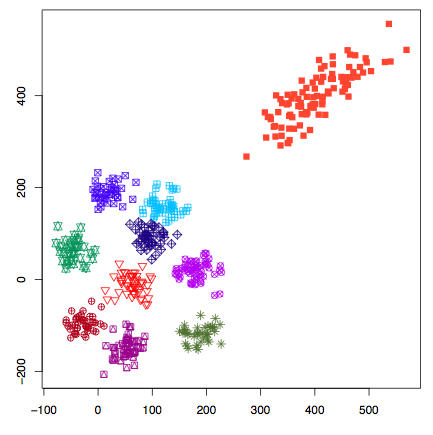
\includegraphics[scale=.4]{../../fig/kmeans0.png}
\end{center}
\end{frame}

\begin{frame}
\frametitle{Step 1: choose initial cluster centers.}
\begin{center}
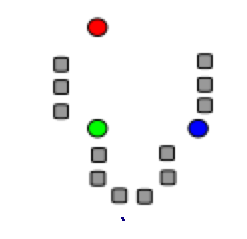
\includegraphics[scale=.6]{../../fig/kmeans1.png}
\end{center}
\begin{itemize}
\item The circles are the cluster means, the squares are the data points, and the color indicates the cluster.
\end{itemize}
\end{frame}

\begin{frame}
\frametitle{Step 2: assign each data point (square) to its closest center (circle).}
\begin{center}
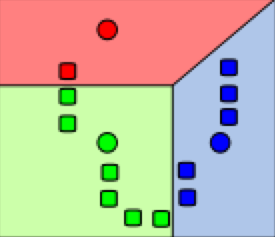
\includegraphics[scale=.6]{../../fig/kmeans2.png}
\end{center}
\end{frame}

\begin{frame}
\frametitle{Step 3: update the cluster centers to be the within-cluster data means.}
\begin{center}
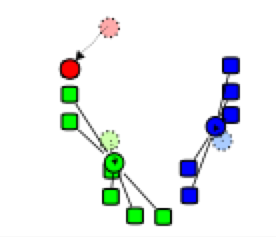
\includegraphics[scale=.6]{../../fig/kmeans3.png}
\end{center}
\end{frame}

\begin{frame}
\frametitle{Repeat step 2: reassign points to their closest cluster centers.}
\begin{center}
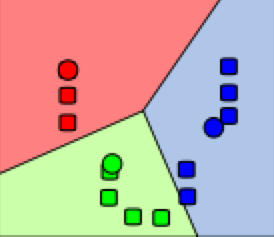
\includegraphics[scale=.6]{../../fig/kmeans4.png}
\end{center}
\begin{itemize}
\item $\ldots$ and repeat until convergence.
\end{itemize}
\end{frame}

\begin{frame}
\frametitle{Parallel K-means}
\begin{itemize}
\item Step 2: assign points to closest cluster centers
\begin{itemize}
\pause \item Spawn $N$ blocks with $K$ threads each.
\pause \item Let thread $(n, k)$ compute the distance between data point $n$ and cluster center $k$.
\pause \item Synchronize threads within each block.
\pause \item Let thread $(n, 1)$ assign data point $n$ to its nearest cluster center.
\end{itemize}
\pause \item Step 3: recompute cluster centers
\begin{itemize}
\pause \item Spawn one block for each cluster.
\pause \item Within each block, compute the mean of the data in the corresponding cluster.
\end{itemize}
\end{itemize}
\end{frame}


\begin{frame}[fragile]
\frametitle{{\tt gpu\_kmeans.cu}}
\begin{lstlisting}[name=km]
#include <stdio.h>
#include <stdlib.h>

#define I(row, col, ncols) (row * ncols + col)

#define CUDA_CALL(x) {if((x) != cudaSuccess){ \
  printf("CUDA error at %s:%d\n",__FILE__,__LINE__); \
  printf("  %s\n", cudaGetErrorString(cudaGetLastError())); \
  exit(EXIT_FAILURE);}} 
\end{lstlisting}
\end{frame}

\begin{frame}[fragile]
\frametitle{{\tt gpu\_kmeans.cu}: step 2}
\begin{lstlisting}[name=km]
__global__ void get_dst(float *dst, float *x, float *y, 
			float *mu_x, float *mu_y){
  int i = blockIdx.x;
  int j = threadIdx.x;

  dst[I(i, j, blockDim.x)] = (x[i] - mu_x[j]) * (x[i] - mu_x[j]);
  dst[I(i, j, blockDim.x)] += (y[i] - mu_y[j]) * (y[i] - mu_y[j]); 
}

__global__ void regroup(int *group, float *dst, int k){
  int i = blockIdx.x;
  int j;
  float min_dst;
  
  min_dst = dst[I(i, 0, k)];
  group[i] = 1;

  for(j = 1; j < k; ++j){
    if(dst[I(i, j, k)] < min_dst){
      min_dst = dst[I(i, j, k)];
      group[i] = j + 1;
    }
  }
}
\end{lstlisting}
\end{frame}





\begin{frame}[fragile]
\frametitle{{\tt gpu\_kmeans.cu}: step 3}
\begin{lstlisting}[name=km]
__global__ void clear(float *sum_x, float *sum_y, int *nx, int *ny){
  int j = threadIdx.x;
  
  sum_x[j] = 0;
  sum_y[j] = 0;
  nx[j] = 0;
  ny[j] = 0;
}

__global__ void recenter_step1(float *sum_x, float *sum_y, int *nx, int *ny,
			       float *x, float *y, int *group, int n){
  int i;
  int j = threadIdx.x;

  for(i = 0; i < n; ++i){
    if(group[i] == (j + 1)){
      sum_x[j] += x[i];
      sum_y[j] += y[i];
      nx[j]++;
      ny[j]++;
    }
  }               
}
\end{lstlisting}
\end{frame}


\begin{frame}[fragile]
\frametitle{{\tt gpu\_kmeans.cu}: step 3}
\begin{lstlisting}[name=km]
__global__ void recenter_step2(float *mu_x, float *mu_y, float *sum_x,
			       float *sum_y, int *nx, int *ny){
  int j = threadIdx.x;

  mu_x[j] = sum_x[j]/nx[j];
  mu_y[j] = sum_y[j]/ny[j];
}

void kmeans(int nreps, int n, int k,
            float *x_d, float *y_d, float *mu_x_d, float *mu_y_d,
            int *group_d, int *nx_d, int *ny_d,
            float *sum_x_d, float *sum_y_d, float *dst_d){
  int i;
  for(i = 0; i < nreps; ++i){
    get_dst<<<n,k>>>(dst_d, x_d, y_d, mu_x_d, mu_y_d);
    regroup<<<n,1>>>(group_d, dst_d, k);
    clear<<<1,k>>>(sum_x_d, sum_y_d, nx_d, ny_d);
    recenter_step1<<<1,k>>>(sum_x_d, sum_y_d, nx_d, ny_d, x_d, y_d, group_d, n);
    recenter_step2<<<1,k>>>(mu_x_d, mu_y_d, sum_x_d, sum_y_d, nx_d, ny_d);
  }
}

void read_data(float **x, float **y, float **mu_x, float **mu_y, int *n, int *k);
void print_results(int *group, float *mu_x, float *mu_y, int n, int k);
\end{lstlisting}
\end{frame}


\begin{frame}[fragile]
\frametitle{{\tt gpu\_kmeans.cu}}
\begin{lstlisting}[name=km]
int main(){
  /* cpu variables */
  int n; /* number of points */
  int k; /* number of clusters */
  int *group;
  float *x = NULL, *y = NULL, *mu_x = NULL, *mu_y = NULL;

  /* gpu variables */
  int *group_d, *nx_d, *ny_d;
  float *x_d, *y_d, *mu_x_d, *mu_y_d, *sum_x_d, *sum_y_d, *dst_d;

  /* read data from files on cpu */
  read_data(&x, &y, &mu_x, &mu_y, &n, &k);

  /* allocate cpu memory */
  group = (int*) malloc(n*sizeof(int));
  
  /* allocate gpu memory */
  CUDA_CALL(cudaMalloc((void**) &group_d,n*sizeof(int)));
  CUDA_CALL(cudaMalloc((void**) &nx_d, k*sizeof(int)));
  CUDA_CALL(cudaMalloc((void**) &ny_d, k*sizeof(int)));
  CUDA_CALL(cudaMalloc((void**) &x_d, n*sizeof(float)));
  CUDA_CALL(cudaMalloc((void**) &y_d, n*sizeof(float)));
  CUDA_CALL(cudaMalloc((void**) &mu_x_d, k*sizeof(float)));
  CUDA_CALL(cudaMalloc((void**) &mu_y_d, k*sizeof(float)));
  CUDA_CALL(cudaMalloc((void**) &sum_x_d, k*sizeof(float)));
  CUDA_CALL(cudaMalloc((void**) &sum_y_d, k*sizeof(float)));
  CUDA_CALL(cudaMalloc((void**) &dst_d, n*k*sizeof(float)));
\end{lstlisting}
\end{frame}

\begin{frame}[fragile]
\frametitle{{\tt gpu\_kmeans.cu}}
\begin{lstlisting}[name=km]
  /* write data to gpu */
  CUDA_CALL(cudaMemcpy(x_d, x, n*sizeof(float), cudaMemcpyHostToDevice));
  CUDA_CALL(cudaMemcpy(y_d, y, n*sizeof(float), cudaMemcpyHostToDevice));
  CUDA_CALL(cudaMemcpy(mu_x_d, mu_x, k*sizeof(float), cudaMemcpyHostToDevice));
  CUDA_CALL(cudaMemcpy(mu_y_d, mu_y, k*sizeof(float), cudaMemcpyHostToDevice));

  /* perform kmeans */
  kmeans(10, n, k, x_d, y_d, mu_x_d, mu_y_d, group_d, nx_d, ny_d, sum_x_d, sum_y_d, dst_d);
  
  /* read back data from gpu */
  CUDA_CALL(cudaMemcpy(group, group_d, n*sizeof(int), cudaMemcpyDeviceToHost));
  CUDA_CALL(cudaMemcpy(mu_x, mu_x_d, k*sizeof(float), cudaMemcpyDeviceToHost));
  CUDA_CALL(cudaMemcpy(mu_y, mu_y_d, k*sizeof(float), cudaMemcpyDeviceToHost));

  /* print results and clean up */  
  print_results(group, mu_x, mu_y, n, k);
\end{lstlisting}
\end{frame}

\begin{frame}[fragile]
\frametitle{{\tt gpu\_kmeans.cu}}
\begin{lstlisting}[name=km]
  free(x);
  free(y);
  free(mu_x);
  free(mu_y);
  free(group);

  CUDA_CALL(cudaFree(x_d));
  CUDA_CALL(cudaFree(y_d));
  CUDA_CALL(cudaFree(mu_x_d));
  CUDA_CALL(cudaFree(mu_y_d));
  CUDA_CALL(cudaFree(group_d));
  CUDA_CALL(cudaFree(nx_d));
  CUDA_CALL(cudaFree(ny_d));
  CUDA_CALL(cudaFree(sum_x_d));
  CUDA_CALL(cudaFree(sum_y_d));
  CUDA_CALL(cudaFree(dst_d));

  return 0;
}

\end{lstlisting}
\end{frame}

\lstset{language = bash}

\begin{frame}[fragile]
\frametitle{Compile, test, and run.}
\begin{itemize}
\item Compile CPU and GPU versions.
\begin{lstlisting}[name=rkm]
> make
gcc kmeans.c -o kmeans -Wall -ansi -pedantic
nvcc gpu_kmeans.cu -o gpu_kmeans --compiler-options -ansi --compiler-options -Wall
\end{lstlisting}
\pause \item Always run through CUDA MEMCHECK.
\begin{lstlisting}[name=rkm]
> cuda-memcheck ./gpu_kmeans
========= CUDA-MEMCHECK
========= ERROR SUMMARY: 0 errors
\end{lstlisting}
\item Check CPU side with Valgrind. Ignore ``errors" and apparent memory leaks on the GPU side.
\begin{lstlisting}[name=rkm]
> valgrind ./gpu_kmeans
==13523== Memcheck, a memory error detector
==13523== Copyright (C) 2002-2010, and GNU GPL'd, by Julian Seward et al.
==13523== Using Valgrind-3.6.0 and LibVEX; rerun with -h for copyright info
==13523== Command: ./gpu_kmeans
==13523== 
==13523== Warning: set address range perms: large range [0x800000000, 0x2100000000) (noaccess)
==13523== Warning: set address range perms: large range [0x2100000000, 0x2800000000) (noaccess)
\end{lstlisting}
\end{itemize}
\end{frame}

\begin{frame}[fragile]
\frametitle{Compile, test, and run.}
\begin{itemize}
\begin{lstlisting}[name=rkm]
==13523== 
==13523== HEAP SUMMARY:
==13523==     in use at exit: 1,308,694 bytes in 2,469 blocks
==13523==   total heap usage: 4,479 allocs, 2,010 frees, 2,952,191 bytes allocated
==13523== 
==13523== LEAK SUMMARY:
==13523==    definitely lost: 16 bytes in 1 blocks
==13523==    indirectly lost: 0 bytes in 0 blocks
==13523==      possibly lost: 33,064 bytes in 242 blocks
==13523==    still reachable: 1,275,614 bytes in 2,226 blocks
==13523==         suppressed: 0 bytes in 0 blocks
==13523== Rerun with --leak-check=full to see details of leaked memory
==13523== 
==13523== For counts of detected and suppressed errors, rerun with: -v
==13523== ERROR SUMMARY: 0 errors from 0 contexts (suppressed: 11 from 9)
\end{lstlisting}
\pause \item Run for real.
\begin{lstlisting}[name=rkm]
> ./gpu_kmeans
\end{lstlisting}
\end{itemize}
\end{frame}

\lstset{language = C}


\begin{frame}[fragile]
\frametitle{Initial clustering: 300 points, 3 clusters}
\begin{center}
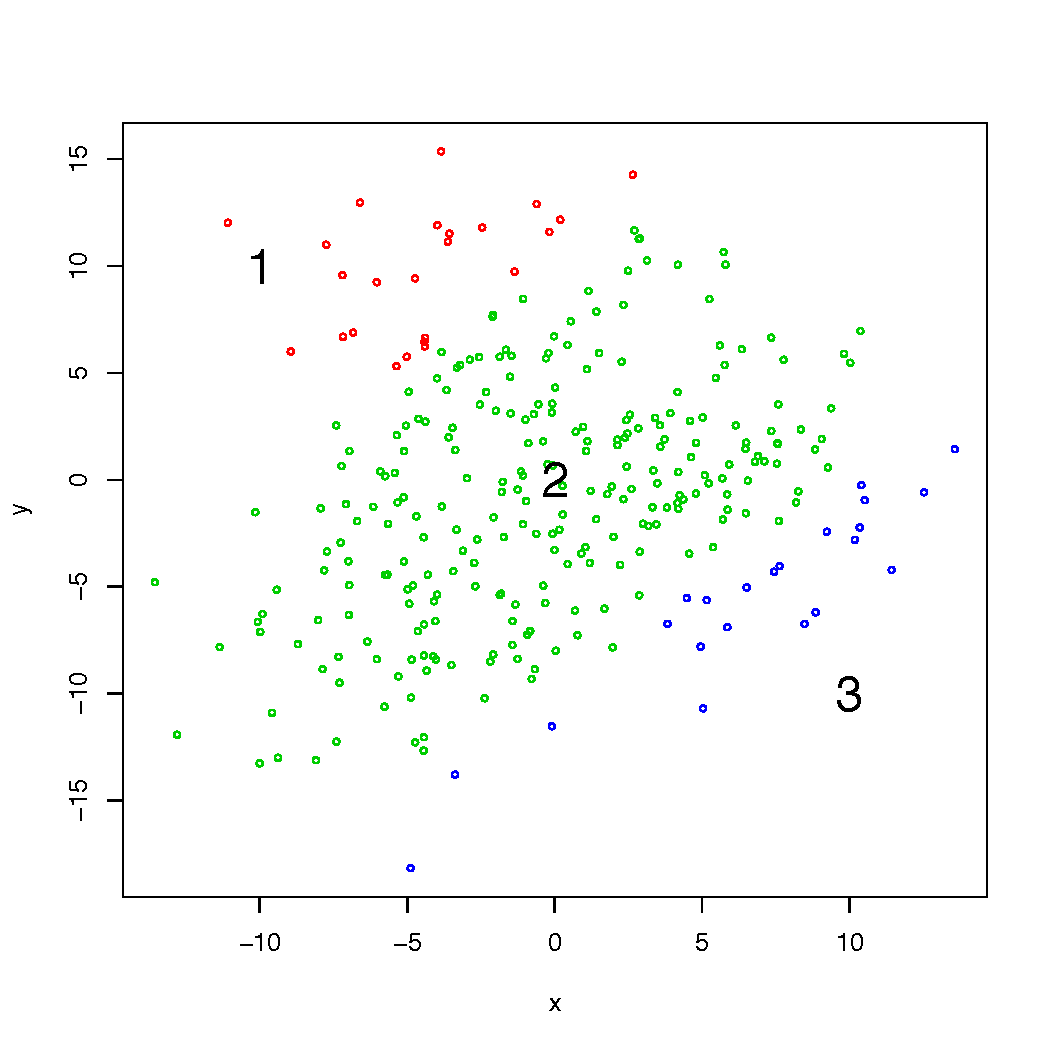
\includegraphics[scale=.5]{../../fig/kmeans-before}
\end{center}
\end{frame}

\begin{frame}[fragile]
\frametitle{Final clustering after 10 iterations}
\begin{center}
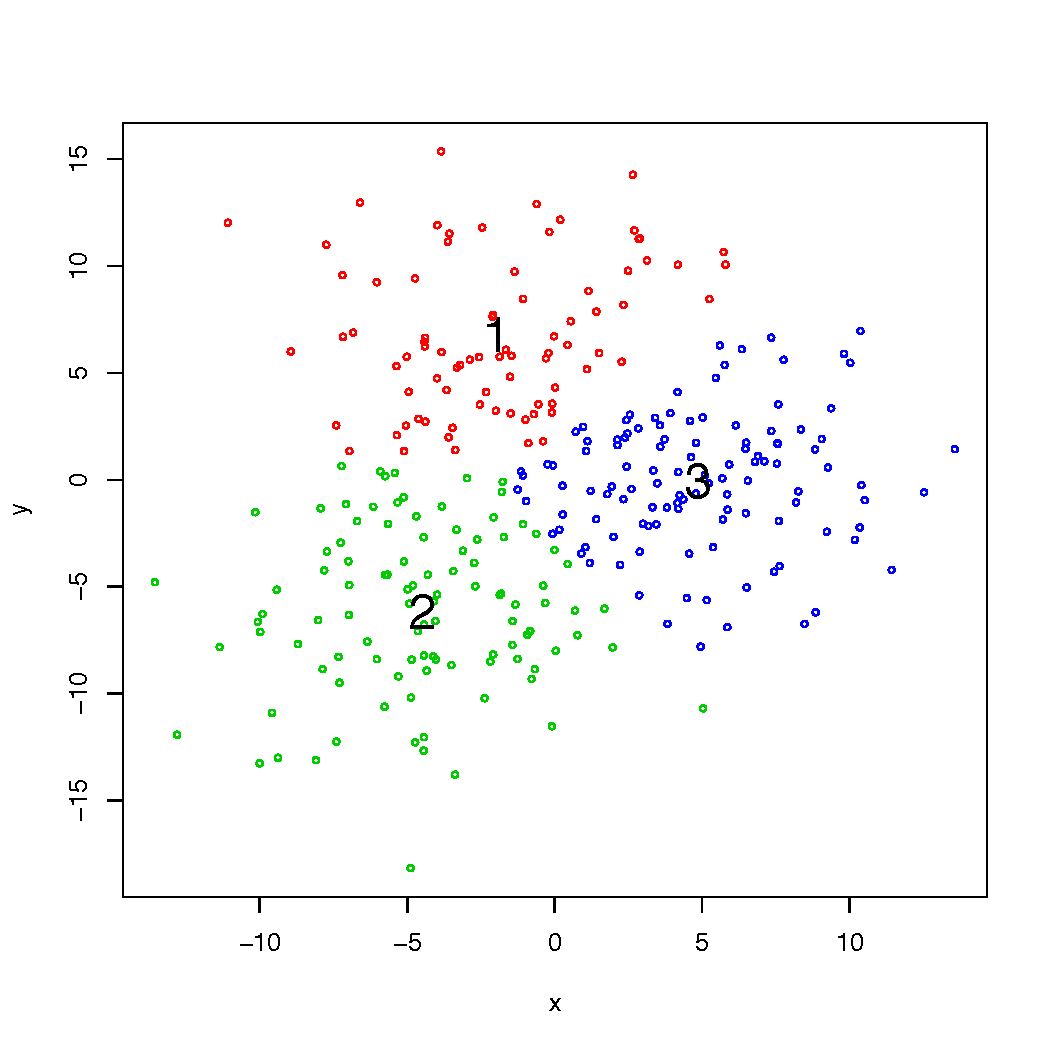
\includegraphics[scale=.5]{../../fig/kmeans-after}
\end{center}
\end{frame}





\subsection{Markov chain Monte Carlo}











\begin{frame}
\frametitle{Markov chain Monte Carlo}
\begin{itemize}
\item Consider a bladder cancer data set:
\begin{itemize}  \scriptsize
\pause \item Available from http://ratecalc.cancer.gov/.
\pause \item Rates of death from bladder cancer of white males from 2000 to 2004 in each county in the USA.
\end{itemize}
\pause \item Let:
\begin{itemize}  \scriptsize
\item $y_k$ = number of observed deaths in county $k$.
\pause \item $n_k$ = the number of person-years in county $k$ divided by 100,000.
\pause \item $\theta_k$ = expected number of deaths per 100,000 person-years.
\end{itemize} 
\pause \item The model:
\begin{align*}
\uncover<7->{y_k} &\uncover<7->{\stackrel{\text{ind}}{\sim} \text{Poisson}(n_k \cdot \theta_k)}\\
\uncover<8->{\theta_k} &\uncover<8->{\stackrel{\text{iid}}{\sim} \text{Gamma}(\alpha, \ \beta)}\\
\uncover<9->{\alpha} & \uncover<9->{\sim \text{Uniform}(0, a_0)} \\
\uncover<10->{\beta} & \uncover<10->{\sim \text{Uniform}(0, b_0)}
\end{align*}
\uncover<11->{\begin{itemize}
\item Also assume that shape $\alpha$ and rate $\beta$ are independent and fix $a_0$ and $b_0$.
\end{itemize}}
\end{itemize}
\end{frame}






\begin{frame}
\frametitle{Full conditional distributions} \scriptsize
\begin{itemize}
\item We want to sample from the joint posterior,
\end{itemize}

\begin{align*}
p(\vc{\theta}, \alpha, \beta \mid \vc{y}) &\propto p(\vc{y} \mid \vc{\theta}, \alpha, \beta) p(\vc{\theta}, \alpha, \beta) \\
&\uncover<2->{\propto p(\vc{y} \mid \vc{\theta}, \alpha, \beta) p(\vc{\theta} \mid \alpha, \beta) p(\alpha, \beta)} \\
&\uncover<3->{\propto p(\vc{y} \mid \vc{\theta}, \alpha, \beta) p(\vc{\theta} \mid \alpha, \beta) p(\alpha)p(\beta)} \\
&\uncover<4->{\propto \prod_{k = 1}^K [p(y_k \mid \theta_k, n_k) p(\theta_k \mid \alpha, \beta)] p(\alpha) p(\beta)} \\
&\uncover<5->{\propto \prod_{k = 1}^K \left [e^{-n_k \theta_k} \theta_k^{y_k} \frac{\beta^\alpha}{\Gamma(\alpha)} \theta_k^{\alpha - 1} e^{-\theta_k \beta}\right ] I(0 < \alpha < a_0) I(0 < \beta < b_0) }
\end{align*}
\begin{itemize}
\uncover<6->{\item We iteratively sample from the full conditional distributions.}
\end{itemize}
\begin{align*}
\uncover<7->{\alpha} &\uncover<8->{\leftarrow p(\alpha \mid \vc{y}, \vc{\theta}, \beta)}  \\
\uncover<8->{\beta} &\uncover<9->{\leftarrow p(\beta \mid \vc{y}, \vc{\theta}, \alpha)} \\
\uncover<9->{\theta_k} &\uncover<7->{\leftarrow p(\theta_k \mid \vc{y}, \vc{\theta}_{-k}, \alpha, \beta) \qquad \Leftarrow \text{IN PARALLEL!}} 
\end{align*}


\end{frame}



\begin{frame}
\frametitle{Full conditional distributions}

\begin{align*}
\uncover<2->{p(\theta_k \mid \vc{y}, \vc{\theta_{-k}}, \alpha, \beta)} & \uncover<2->{\propto p(\vc{\theta}, \alpha, \beta \mid \vc{y})} \\
&\uncover<3->{\propto e^{-n_k \theta_k} \theta_k^{y_k} \theta_k^{\alpha - 1} e^{- \theta_k} \beta} \\
&\uncover<4->{= \theta_k^{y_k + \alpha - 1} e^{-\theta_k(n_k + \beta)}} \\
&\uncover<5->{\propto \text{Gamma}(y_k + \alpha, \ n_k + \beta)}
\end{align*}
\end{frame}


\begin{frame} 
\frametitle{Conditional distributions of $\alpha$ and $\beta$} \small
\begin{align*}
p(\alpha \mid \vc{y}, \vc{\theta}, \beta) &\propto p(\vc{\theta}, \alpha, \beta \mid \vc{y}) \\
&\uncover<2->{\propto \prod_{k = 1}^K \left [ \theta_k^{\alpha - 1} \frac{\beta^\alpha}{\Gamma(\alpha)} \right ] I(0 < \alpha < a_0)} \\
&\uncover<3->{=\left (\prod_{k = 1}^K \theta_k \right )^\alpha \beta^{K \alpha} \Gamma(\alpha)^{-K} I(0 < \alpha < a_0)} \\ \\
\uncover<4->{p(\beta \mid \vc{y}, \vc{\theta}, \alpha)} &\uncover<4->{\propto p(\vc{\theta}, \alpha, \beta \mid \vc{y})} \\
&\uncover<5->{\propto \prod_{k = 1}^K \left [ e^{-\theta_k \beta} \beta^\alpha \right ] I(0 < \beta < b_0)} \\
&\uncover<6->{=\beta^{K \alpha} e^{- \beta \sum_{k = 1}^K \theta_k} I(0 < \beta < b_0)} \\
&\uncover<7->{\propto \text{Gamma}\left (K \alpha + 1, \ \sum_{k = 1}^K \theta_k \right) I(0 < \beta < b_0)}
\end{align*}
\end{frame}




\begin{frame}
\frametitle{Summarizing the Gibbs sampler}
\begin{enumerate}
\item Sample $\vc{\theta}$ from from its full conditional.
\begin{itemize}
\pause \item Draw the $\theta_k$'s \emph{in parallel} from independent Gamma($y_k + \alpha$, $n_k + \beta$) distributions.
\pause \item In other words, assign each thread to draw an individual $\theta_k$ from its Gamma($y_k + \alpha$, $n_k + \beta$) distribution.
\end{itemize}
\pause \item Sample $\alpha$ from its full conditional using a random walk Metropolis step.
\pause \item Sample $\beta$ from its full conditional (truncated Gamma) using the inverse cdf method if $b_0$ is low or a non-truncated Gamma if $b_0$ is high.
\end{enumerate}

\end{frame}















\begin{frame}
\frametitle{The gamma sampler for $\beta$ and $\theta_1, \ldots, \theta_K$}
\begin{itemize} \small
\item Taken from Marsaglia and Tsang (2001).
\pause \item Rejection sampler with acceptance rate $\ge 95\%$ when the shape parameter is $\ge 1$.
\pause \item Steps for a Gamma($a$, 1) sampler:
\begin{enumerate} \small
\pause \item Let $d = a - 1/3$ and $c = 1 / \sqrt{9 d}$.
\pause \item Draw $x \sim $ Normal(0, 1) and let $v = (1 + c \cdot x)^3$. Repeat if $v \le 0$.
\pause \item Let $u \sim $ Uniform(0, 1).
\pause \item If $u < 1 - 0.0331 \cdot x^4$, return $d \cdot v$.
\pause \item If $\log(u) < 0.5 \cdot x^2 + d \cdot (1 - v + \log(v))$, return $d \cdot v$.
\pause \item Go to step 2.
\end{enumerate}
\end{itemize}
\end{frame}

\begin{frame}
\frametitle{The metropolis step for $\alpha$}
\begin{itemize} \scriptsize
\item The goal is to sample from the full conditional distribution,
\begin{align*}
p(\alpha \mid \vc{y}, \vc{\theta}, \beta) \propto \left ( \prod_{k = 1}^K \theta_k \right )^\alpha \beta^{K \alpha} \Gamma(\alpha)^{-K} I(0 < \alpha < a_0)
\end{align*}
\pause \item Let $\alpha^{(j)}$ be the last sampled value of $\alpha$. Sample $\alpha^{(j + 1)}$ as follows:

\begin{enumerate} \scriptsize
\pause \item Draw $\alpha^* \sim N(\alpha^{(j)}, \ \sigma^2$), where $\sigma^2$ is a tuning parameter.
\pause \item If $\alpha^* < 0$ or $\alpha^* > a_0$, let $p = 0$. Otherwise,
\end{enumerate}

\pause \begin{align*}
p = \frac{p(\alpha^* \mid \vc{y}, \vc{\theta}, \beta)}{p(\alpha^{(j)} \mid \vc{y}, \vc{\theta}, \beta)} = \left ( \prod_{k = 1}^K \theta_k \right )^{\alpha^* - \alpha^{(j)}} \beta^{K(\alpha^* - \alpha^{(j)})} \left( \frac{\Gamma(\alpha^*)}{\Gamma(\alpha^{(j)})} \right )^{-K}
\end{align*}
\begin{enumerate} \setcounter{enumi}{2} \scriptsize
\pause \item Draw $u \sim U(0, 1)$.
\pause \item If $u < p$, $\alpha^{(j + 1)} = \alpha^*$. Otherwise, $\alpha^{(j + 1)} = \alpha^{(j)}$.
\pause \item Raise $\sigma^2$ if $\alpha^*$ was accepted and lower $\sigma^2$ if $\alpha^*$ was rejected. The optimal acceptance rate is roughly 44\%.
\end{enumerate}
\end{itemize}
\end{frame}













\begin{frame}[fragile]
\frametitle{Zebulun Arendsee's implementation}
\begin{lstlisting}[name=mc]
/*
Created by Zebulun Arendsee.
March 26, 2013

Modified by Will Landau.
June 30, 2013
will-landau.com
landau@iastate.edu

This program implements a MCMC algorithm for the following hierarchical
model:

y_k     ~ Poisson(n_k * theta_k)     k = 1, ..., K
theta_k ~ Gamma(a, b)
a       ~ Unif(0, a0)
b       ~ Unif(0, b0) 

We let a0 and b0 be arbitrarily large.

Arguments:
    1) input filename
        With two space delimited columns holding integer values for
        y and float values for n.
    2) number of trials (1000 by default)

Output: A comma delimited file containing a column for a, b, and each
theta. All output is written to stdout. */
\end{lstlisting}
\end{frame}

\begin{frame}[fragile]
\frametitle{Zebulun Arendsee's implementation}
\begin{lstlisting}[name=mc]
/*
Example dataset:

$ head -3 data.txt
4 0.91643
23 3.23709
7 0.40103

 Example of compilation and execution:

$ nvcc gibbs_metropolis.cu -o gibbs
$ ./gibbs mydata.txt 2500 > output.csv
$

This code borrows from the nVidia developer zone documentation, 
specifically http://docs.nvidia.com/cuda/curand/index.html#topic_1_2_1
*/

#include <stdio.h>
#include <stdlib.h>
#include <cuda.h>
#include <math.h>
#include <curand_kernel.h>
#include <thrust/reduce.h>

#define PI 3.14159265359f
#define THREADS_PER_BLOCK 64
\end{lstlisting}
\end{frame}

\begin{frame}[fragile]
\frametitle{Zebulun Arendsee's implementation}
\begin{lstlisting}[name=mc]
#define CUDA_CALL(x) {if((x) != cudaSuccess){ \
  printf("CUDA error at %s:%d\n",__FILE__,__LINE__); \
  printf("  %s\n", cudaGetErrorString(cudaGetLastError())); \
  exit(EXIT_FAILURE);}} 

#define CURAND_CALL(x) {if((x) != CURAND_STATUS_SUCCESS) { \
  printf("Error at %s:%d\n",__FILE__,__LINE__); \
  printf("  %s\n", cudaGetErrorString(cudaGetLastError())); \
  exit(EXIT_FAILURE);}}

__host__ void load_data(int argc, char **argv, int *K, int **y, float **n);

__host__ float sample_a(float a, float b, int K, float sum_logs);
__host__ float sample_b(float a, int K, float flat_sum);

__host__ float rnorm();
__host__ float rgamma(float a, float b);

__device__ float rgamma(curandState *state, int id, float a, float b);

__global__ void sample_theta(curandState *state, float *theta, float *log_theta,  int *y, float *n, float a, float b, int K);
__global__ void setup_kernel(curandState *state, unsigned int seed, int);
\end{lstlisting}
\end{frame}

\begin{frame}[fragile]
\frametitle{Zebulun Arendsee's implementation}
\begin{lstlisting}[name=mc]
int main(int argc, char **argv){

  curandState *devStates;
  float a, b, flat_sum, sum_logs, *n, *dev_n, *dev_theta, *dev_log_theta;
  int i, K, *y, *dev_y, nBlocks, trials = 1000;

  if(argc > 2)
    trials = atoi(argv[2]);

  load_data(argc, argv, &K, &y, &n);


  /*------ Allocate memory -----------------------------------------*/

  CUDA_CALL(cudaMalloc((void **)&dev_y, K * sizeof(int)));
  CUDA_CALL(cudaMemcpy(dev_y, y, K * sizeof(int), 
            cudaMemcpyHostToDevice));

  CUDA_CALL(cudaMalloc((void **)&dev_n, K * sizeof(float)));
  CUDA_CALL(cudaMemcpy(dev_n, n, K * sizeof(float), 
            cudaMemcpyHostToDevice));

  /* Allocate space for theta and log_theta on device and host */
  CUDA_CALL(cudaMalloc((void **)&dev_theta, K * sizeof(float)));
  CUDA_CALL(cudaMalloc((void **)&dev_log_theta, K * sizeof(float)));

  /* Allocate space for random states on device */
  CUDA_CALL(cudaMalloc((void **)&devStates, K * sizeof(curandState)));
\end{lstlisting}
\end{frame}

\begin{frame}[fragile]
\frametitle{Zebulun Arendsee's implementation}
\begin{lstlisting}[name=mc]
  /*------ Setup random number generators (one per thread) ---------*/

  nBlocks = (K + THREADS_PER_BLOCK - 1) / THREADS_PER_BLOCK;
  setup_kernel<<<nBlocks, THREADS_PER_BLOCK>>>(devStates, 0, K);

\end{lstlisting}
\end{frame}

\begin{frame}[fragile]
\frametitle{Zebulun Arendsee's implementation}
\begin{lstlisting}[name=mc]
  /*------ MCMC ----------------------------------------------------*/
    
  printf("alpha, beta\n");

  /* starting values of hyperparameters */
  a = 20; 
  b = 1; 

  /* Steps of MCMC */  
  for(i = 0; i < trials; i++){    
    sample_theta<<<nBlocks, THREADS_PER_BLOCK>>>(devStates, dev_theta, dev_log_theta, dev_y, dev_n, a, b, K);

    /* print hyperparameters. */
    printf("%f, %f\n", a, b);

    /* Make iterators for thetas and log thetas. */
    thrust::device_ptr<float> theta(dev_theta);
    thrust::device_ptr<float> log_theta(dev_log_theta);
    
    /* Compute pairwise sums of thetas and log_thetas. */
    flat_sum = thrust::reduce(theta, theta + K);
    sum_logs = thrust::reduce(log_theta, log_theta + K);
  
    /* Sample hyperparameters. */
    a = sample_a(a, b, K, sum_logs);
    b = sample_b(a, K, flat_sum);
  }
\end{lstlisting}
\end{frame}

\begin{frame}[fragile]
\frametitle{Zebulun Arendsee's implementation}
\begin{lstlisting}[name=mc]
  /*------ Free Memory -------------------------------------------*/

  free(y);
  free(n);

  CUDA_CALL(cudaFree(devStates));
  CUDA_CALL(cudaFree(dev_theta));
  CUDA_CALL(cudaFree(dev_log_theta));
  CUDA_CALL(cudaFree(dev_y));
  CUDA_CALL(cudaFree(dev_n));

  return EXIT_SUCCESS;
}
\end{lstlisting}
\end{frame}

\begin{frame}[fragile]
\frametitle{Zebulun Arendsee's implementation}
\begin{lstlisting}[name=mc]
/*
 *  Metropolis algorithm for producing random a values. 
 *  The proposal distribution in normal with a variance that
 *  is adjusted at each step.
 */
 
__host__ float sample_a(float a, float b, int K, float sum_logs){

  static float sigma = 2;
  float U, log_acceptance_ratio, proposal = rnorm() * sigma + a;

  if(proposal <= 0) 
    return a;

  log_acceptance_ratio = (proposal - a) * sum_logs +
                         K * (proposal - a) * log(b) -
                         K * (lgamma(proposal) - lgamma(a));

  U = rand() / float(RAND_MAX);

  if(log(U) < log_acceptance_ratio){
    sigma *= 1.1;
    return proposal;
  } else {
    sigma /= 1.1;
    return a;
  }
}
\end{lstlisting}
\end{frame}

\begin{frame}[fragile]
\frametitle{Zebulun Arendsee's implementation}
\begin{lstlisting}[name=mc]
/*
 *  Sample b from a gamma distribution.
 */

__host__ float sample_b(float a, int K, float flat_sum){

  float hyperA = K * a + 1;
  float hyperB = flat_sum;
  return rgamma(hyperA, hyperB);
}

 
__host__ float rnorm(){

  float U1 = rand() / float(RAND_MAX);
  float U2 = rand() / float(RAND_MAX);
  float V1 = sqrt(-2 * log(U1)) * cos(2 * PI * U2);
  /* float V2 = sqrt(-2 * log(U2)) * cos(2 * PI * U1); */
  return V1;
}
\end{lstlisting}
\end{frame}

\begin{frame}[fragile]
\frametitle{Zebulun Arendsee's implementation}
\begin{lstlisting}[name=mc]
__host__ float rgamma(float a, float b){

  float d = a - 1.0 / 3;
  float Y, U, v;

  while(1){
    Y = rnorm();
    v = pow((1 + Y / sqrt(9 * d)), 3);

    /* Necessary to avoid taking the log of a negative number later. */
    if(v <= 0) 
      continue;
        
    U = rand() / float(RAND_MAX);

    /* Accept the sample under the following condition. 
       Otherwise repeat loop. */
    if(log(U) < 0.5 * pow(Y,2) + d * (1 - v + log(v)))
            return d * v / b;
  }
}
\end{lstlisting}
\end{frame}

\begin{frame}[fragile]
\frametitle{Zebulun Arendsee's implementation}
\begin{lstlisting}[name=mc]
__device__ float rgamma(curandState *state, int id, float a, float b){

  float d = a - 1.0 / 3;
  float Y, U, v;

  while(1){   
    Y = curand_normal(&state[id]);
    v = pow((1 + Y / sqrt(9 * d)), 3);

    /* Necessary to avoid taking the log of a negative number later. */
    if(v <= 0) 
      continue;
        
    U = curand_uniform(&state[id]);

    /* Accept the sample under the following condition. 
       Otherwise repeat loop. */
    if(log(U) < 0.5 * pow(Y,2) + d * (1 - v + log(v)))
      return d * v / b;
  }
}
\end{lstlisting}
\end{frame}



\begin{frame}[fragile]
\frametitle{Zebulun Arendsee's implementation}
\begin{lstlisting}[name=mc]
/*
 *  Sample each theta from the appropriate gamma distribution
 */
 
__global__ void sample_theta(curandState *state,  float *theta, 
                             float *log_theta, int *y, float *n, float a, float b, int K){
                             
  int id = threadIdx.x + blockIdx.x * blockDim.x;
  float hyperA, hyperB;
    
  if(id < K){
    hyperA = a + y[id];
    hyperB = b + n[id];
    theta[id] = rgamma(state, id, hyperA, hyperB);
    log_theta[id] = log(theta[id]);
  }
}

/* 
 *  Initialize GPU random number generators 
 */
 
__global__ void setup_kernel(curandState *state, unsigned int seed, int K){
  int id = threadIdx.x + blockIdx.x * blockDim.x;
  if(id < K)
    curand_init(seed, id, 0, &state[id]);
}
\end{lstlisting}
\end{frame}

\lstset{language = bash, basicstyle = \tiny}

\begin{frame}[fragile]
\frametitle{Compile, test, and run.}
\begin{itemize}
\item Compile, requiring compute capability 2.0 or above. 
\begin{lstlisting}[name=tmc]
> nvcc -arch=sm_20 gibbs_metropolis.cu -o gibbs_metropolis
\end{lstlisting}
\pause \item Always check with CUDA MEMCHECK.
\begin{lstlisting}[name=tmc]
> cuda-memcheck ./gibbs_metropolis smallData.txt 10
========= CUDA-MEMCHECK
alpha, beta
19.070215, 1.226651
19.441961, 1.521381
16.017313, 1.413954
11.898635, 1.253917
11.898635, 1.767045
13.532320, 1.783169
13.532320, 1.648099
13.532320, 2.005379
13.532320, 2.136331
12.914721, 1.408586
========= ERROR SUMMARY: 0 errors 
\end{lstlisting}
\end{itemize}
\end{frame}

\begin{frame}[fragile]
\frametitle{Compile, test, and run.}
\begin{itemize}
\item Check CPU side with Valgrind. Ignore ``errors" from GPU code.
\begin{lstlisting}[name=tmc]
> valgrind ./gibbs_metropolis smallData.txt 10
==12942== Memcheck, a memory error detector
==12942== Copyright (C) 2002-2010, and GNU GPL'd, by Julian Seward et al.
==12942== Using Valgrind-3.6.0 and LibVEX; rerun with -h for copyright info
==12942== Command: ./gibbs_metropolis smallData.txt 10
==12942== 
==12942== Warning: set address range perms: large range [0x800000000, 0x2100000000) (noaccess)
==12942== Warning: set address range perms: large range [0x2100000000, 0x2800000000) (noaccess)
alpha, beta
19.070215, 1.226651
19.441961, 1.521381
16.017313, 1.413954
11.898635, 1.253917
11.898635, 1.767045
13.532320, 1.783169
13.532320, 1.648099
13.532320, 2.005379
13.532320, 2.136331
12.914721, 1.408586
\end{lstlisting}
\end{itemize}
\end{frame}

\begin{frame}[fragile]
\frametitle{Compile, test, and run.}
\begin{itemize}
\begin{lstlisting}[name=tmc]
==12942== 
==12942== HEAP SUMMARY:
==12942==     in use at exit: 1,453,685 bytes in 2,647 blocks
==12942==   total heap usage: 4,175 allocs, 1,528 frees, 2,706,460 bytes allocated
==12942== 
==12942== LEAK SUMMARY:
==12942==    definitely lost: 16 bytes in 1 blocks
==12942==    indirectly lost: 0 bytes in 0 blocks
==12942==      possibly lost: 39,184 bytes in 287 blocks
==12942==    still reachable: 1,414,485 bytes in 2,359 blocks
==12942==         suppressed: 0 bytes in 0 blocks
==12942== Rerun with --leak-check=full to see details of leaked memory
==12942== 
==12942== For counts of detected and suppressed errors, rerun with: -v
==12942== ERROR SUMMARY: 0 errors from 0 contexts (suppressed: 11 from 9)
\end{lstlisting}
\pause \item Run 2 chains for real.
\begin{lstlisting}[name=tmc]
> ./gibbs_metropolis data.txt 10000 > chain1.txt
> ./gibbs_metropolis data.txt 10000 > chain2.txt
\end{lstlisting}
\end{itemize}
\end{frame}



\begin{frame}
\frametitle{Diagnostics: Gelman-Rubin potential scale reduction factor}
\begin{align*}
\wh{R}  = \sqrt{\frac{\frac{n-1}{n} W + \frac{1}{n} B}{W}} \approx \sqrt{1 + \frac{B}{nW}}
\end{align*}
\begin{itemize}
\pause \item $n$ is the number of chains, $B$ is the between-chain variability, and $W$ is the within-chain variability.
\pause \item $\wh{R} > 1.1$ is evidence of a lack of convergence.
\pause \item For 2 chains, each with 10000 iterations (including 2000 iterations of burn-in), 
\begin{center}
\begin{tabular}{l|l|l}
& Point est $\wh{R}$ & Upper 95\% CI $\wh{R}$ \\ \hline
$\alpha$ & 1.02 & 1.08 \\
$\beta$ & 1.02 & 1.08
\end{tabular}
\end{center}
\end{itemize}
\end{frame}

\begin{frame}
\frametitle{Diagnostics: trace plots after burn-in}
\begin{center}
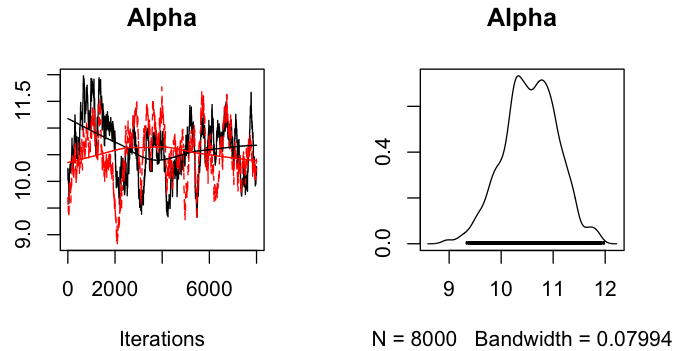
\includegraphics[scale=.3]{../../fig/mcmc-trace-alpha.png} \\
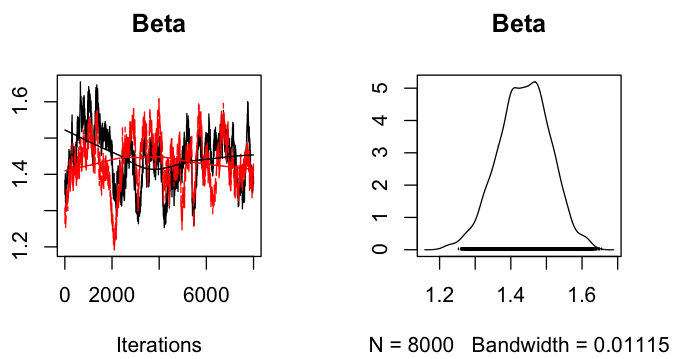
\includegraphics[scale=.3]{../../fig/mcmc-trace-beta.png}
\end{center}
\end{frame}





\subsection{Ordinary least squares}

\begin{frame}
\frametitle{Example: {\tt ols.cu}}

\begin{itemize}
\item I will attempt to solve the least squares problem,


\begin{align*}
\vc{y} = X \vc{ \beta} + \vc{\e} 
\end{align*}

by computing the solution,

\begin{align*}
\wh{\vc{\beta}} = (X^T X)^{-1}X^T \vc{y}
\end{align*}
\end{itemize}
\end{frame}


\begin{frame}[fragile]
\frametitle{Example: {\tt ols.cu}}  \lstset{basicstyle=\tiny}
\begin{lstlisting}[name=ols]
#include <stdio.h>
#include <stdlib.h>
#include <string.h>
#include <cuda_runtime.h>
#include <cublas_v2.h>
#include <cula.h>
#include <math.h>

#define I(i, j, ld) j * ld + i

#define CUDA_CALL(x) {if((x) != cudaSuccess){ \
  printf("CUDA error at %s:%d\n",__FILE__,__LINE__); \
  printf("  %s\n", cudaGetErrorString(cudaGetLastError())); \
  exit(EXIT_FAILURE);}} 

float rnorm(){
  float r1 = ((float) rand()) / ((float) RAND_MAX);
  float r2 = ((float) rand()) / ((float) RAND_MAX);
  return sqrt( -2 * log(r1) ) * cos(2 * 3.1415 * r2);
}

int main(){
  int i, j;
  int n = 10;
  int p = 3;
  int* ipiv;
  float k;
  float *X, *XtX, *XtY, *beta, *Y, *dX, *dXtX, *dXtY, *dbeta, *dY;
\end{lstlisting}
\end{frame}


\begin{frame}[fragile]
\frametitle{Example: {\tt ols.cu}}  \lstset{basicstyle=\tiny}
\begin{lstlisting}[name=ols]
  float *a, *b;
  a = (float*) malloc(sizeof(*X));
  b = (float*) malloc(sizeof(*X));
  *a = 1.0;
  *b = 0.0;

  cublasHandle_t handle;
  cublasCreate(&handle);

  X = (float*) malloc(n * p * sizeof(*X));
  XtX = (float*) malloc(p * p * sizeof(*X));
  XtY = (float*) malloc(p * sizeof(*X));
  beta = (float*) malloc(p * sizeof(*X));
  Y = (float*) malloc(n * sizeof(*X));
  
  CUDA_CALL(cudaMalloc((void**) &ipiv, p * p * sizeof(*ipiv)));
  CUDA_CALL(cudaMalloc((void**) &dX, n * p * sizeof(*X)));
  CUDA_CALL(cudaMalloc((void**) &dXtX, p * p * sizeof(*X)));
  CUDA_CALL(cudaMalloc((void**) &dXtY, p * sizeof(*X)));
  CUDA_CALL(cudaMalloc((void**) &dbeta, p * sizeof(*X)));
  CUDA_CALL(cudaMalloc((void**) &dY, n * sizeof(*X)));
 
\end{lstlisting}
\end{frame}



\begin{frame}[fragile]
\frametitle{Example: {\tt ols.cu}}  \lstset{basicstyle=\tiny}
\begin{lstlisting}[name=ols]
  printf("Y\t\tX\n");
  for(i = 0; i < n; i++){
    k = (float) i;
    X[I(i, 0, n)] = 1.0;
    X[I(i, 1, n)] = k / 10.0;
    X[I(i, 2, n)] = k * k / 10.0;  
    Y[i] = (k - 5.0) * (k - 2.3) / 3.0 + rnorm();
    
    printf("%0.2f\t\t", Y[i]);
    for(j = 0; j < p; j++){
      printf("%0.2f\t", X[I(i, j, n)]);
    } 
    printf("\n");
  }
  printf("\n");

  CUDA_CALL(cudaMemcpy(dX, X, n * p * sizeof(float), cudaMemcpyHostToDevice));
  CUDA_CALL(cudaMemcpy(dY, Y, n * sizeof(float), cudaMemcpyHostToDevice));

  cublasSgemm(handle, CUBLAS_OP_T, CUBLAS_OP_N, p, p, n, 
    a, dX, n, dX, n, b, dXtX, p);

  CUDA_CALL(cudaMemcpy(XtX, dXtX, p * p * sizeof(float), cudaMemcpyDeviceToHost));
\end{lstlisting}
\end{frame}

\begin{frame}[fragile]
\frametitle{Example: {\tt ols.cu}}  \lstset{basicstyle=\tiny}
\begin{lstlisting}[name=ols]
  printf("XtX\n");
  for(i = 0; i < p; i++){
    for(j = 0; j < p; j++){
      printf("%0.2f\t", XtX[I(i, j, p)]);
    }
    printf("\n");
  }
  printf("\n");
\end{lstlisting}
\end{frame}

\begin{frame}[fragile]
\frametitle{Output of code so far}  \lstset{basicstyle=\tiny}

\begin{lstlisting}[name=tols]
> nvcc -I /usr/local/cula/include -L /usr/local/cula/lib64 -lcula_core -lcula_lapack -lcublas -lcudart ols.cu -o ols
> ./ols
Y		X
3.37		1.00	0.00	0.00	
1.94		1.00	0.10	0.10	
0.44		1.00	0.20	0.40	
-0.30		1.00	0.30	0.90	
-2.08		1.00	0.40	1.60	
-0.84		1.00	0.50	2.50	
-0.18		1.00	0.60	3.60	
3.40		1.00	0.70	4.90	
5.51		1.00	0.80	6.40	
7.39		1.00	0.90	8.10	

XtX
10.00	4.50	28.50	
4.50	2.85	20.25	
28.50	20.25	153.33	
\end{lstlisting}
\end{frame}


\begin{frame}[fragile]
\frametitle{Example: {\tt ols.cu}}
\begin{itemize}
\item We have $X^T X$, but which we need to invert in order to compute our solution,
\pause \begin{align*}
\wh{\vc{\beta}} = (X^T X)^{-1}X^T \vc{y}
\end{align*}
\pause \item But CUBLAS can only invert triangular matrices!
\end{itemize}
\end{frame}

\begin{frame}[fragile]
\frametitle{Enter CULA: CUDA LAPACK} \lstset{basicstyle=\tiny}
\begin{lstlisting}[name=ols]
  culaInitialize();
  
  culaDeviceSgetrf(p, p, dXtX, p, ipiv);
  culaDeviceSgetri(p, dXtX, p, ipiv);
  
  CUDA_CALL(cudaMemcpy(XtX, dXtX, p * p * sizeof(float), cudaMemcpyDeviceToHost));

  printf("XtX^(-1)\n");
  for(i = 0; i < p; i++){
    for(j = 0; j < p; j++){
      printf("%0.2f\t", XtX[I(i, j, p)]);
    }
    printf("\n");
  }
  printf("\n");

  cublasSgemm(handle, CUBLAS_OP_T, CUBLAS_OP_N, p, 1, n, 
    a, dX, n, dY, n, b, dXtY, p);

  cublasSgemv(handle, CUBLAS_OP_N, p, p, 
    a, dXtX, p, dXtY, 1, b, dbeta, 1);

  CUDA_CALL(cudaMemcpy(beta, dbeta, p * sizeof(float), cudaMemcpyDeviceToHost));

  printf("CUBLAS/CULA matrix algebra parameter estimates:\n");
  for(i = 0; i < p; i++){
    printf("beta_%i = %0.2f\n", i, beta[i]);
  }
  printf("\n");
\end{lstlisting}
\end{frame}

\begin{frame}[fragile]
\frametitle{CULA's {\tt culaSgels()} does least squares for you}  \lstset{basicstyle=\tiny}
\begin{lstlisting}[name=ols]
  culaSgels('N', n, p, 1, X, n, Y, n);

  printf("culaSgels Parameter estimates:\n");
  for(i = 0; i < p; i++){
    printf("beta_%i = %0.2f\n", i, Y[i]);
  }
  printf("\n");

  culaShutdown();
  cublasDestroy(handle);

  free(a);
  free(b);
  free(X);
  free(XtX);
  free(XtY);
  free(beta);
  free(Y);

  CUDA_CALL(cudaFree(dX));
  CUDA_CALL(cudaFree(dXtX));
  CUDA_CALL(cudaFree(dXtY));
  CUDA_CALL(cudaFree(dbeta));
  CUDA_CALL(cudaFree(dY));
}
\end{lstlisting}
\end{frame}

\begin{frame}[fragile]
\frametitle{Rest of the output}
\begin{lstlisting}[name=tols]
XtX^(-1)
0.62	-2.59	0.23	
-2.59	16.55	-1.70	
0.23	-1.70	0.19	

CUBLAS/CULA matrix algebra parameter estimates:
beta_0 = 3.78
beta_1 = -25.53
beta_2 = 3.36

culaSgels Parameter estimates:
beta_0 = 3.78
beta_1 = -25.53
beta_2 = 3.36
\end{lstlisting}
\end{frame}


\begin{frame}
\frametitle{Resources} \small
\begin{enumerate}
\item J. Sanders and E. Kandrot. {CUDA by Example.} Addison-Wesley, 2010.
\pause \item D. Kirk, W.H. Wen-mei, and W. Hwu. \emph{Programming massively parallel processors: a hands-on approach.} Morgan Kaufmann, 2010.
\pause \item A. Lee, C. Yau, M.B. Giles, A. Doucet, and C.C. Holmes. On the utility of graphics cards to perform massively parallel simulation of advanced monte carlo methods. \emph{Journal of Computational and Graphical Statistics}, 19(4): 769-789, 2010.
\pause \item M.A. Suchard, Q. Wang, C. Chan, J. Frelinger, A. Cron, and M. West. Understanding gpu programming for statistical computation: Studies in massively parallel mixtures. \emph{Journal of Computational and Graphical Statistics.} 19(2): 419-438, 2010.
\end{enumerate}
\end{frame}

\begin{frame}
\frametitle{Outline}
\tableofcontents
\end{frame}

\begin{frame}
\frametitle{Resources} \small
\begin{enumerate} \setcounter{enumi}{4}
\item \url{http://docs.nvidia.com/cuda/index.html}
\pause \item \url{https://developer.nvidia.com/gpu-accelerated-libraries}
\pause \item Dr. Ranjan Maitra's STAT 580 notes.
\pause \item \href{http://jarad.me/stat544/archive.html}{Dr. Jarad Niemi's STAT 544 notes.}
\pause \item Andrew Gelman, John B. Carlin, Hal S. Stern, and Donald B. Rubin. \emph{Bayesian Data Analysis}. 2nd ed. Chapman \& Hall/CRC, 2004.
\pause \item George Marsaglia and Wai Wan Tsang. ``A Simple Method for Generating Gamma Variables." \emph{ACM Transactions on Mathematical Software} 26(3), Sept 2000. 363-372.
\end{enumerate}
\end{frame}


\begin{frame}
\frametitle{Example code} \small
\begin{enumerate}
\item \href{http://will-landau.com/gpu/Code/CUDA_C/vectorsums/vectorsums.cu}{vectorsums.cu}
\item \href{http://will-landau.com/gpu/Code/CUDA_C/pairwise_sum/pairwise_sum.cu}{pairwise\_sum.cu}
\item \href{http://will-landau.com/gpu/Code/CUDA_C/kmeans/kmeans.zip}{kmeans.zip}
\item \href{http://will-landau.com/gpu/Code/CUDA_C/mcmc/mcmc.zip}{mcmc.zip}
\item \href{http://will-landau.com/gpu/Code/CUDA_C/CULA/ols/ols.cu}{ols.cu}
\end{enumerate}
\end{frame}

\begin{frame}
\frametitle{That's all.}
\begin{itemize}
\item Series materials are available at \url{http://will-landau.com/gpu}.
\end{itemize}

\end{frame}

\end{document}